% !TEX program = xelatex
% =====================================================================
% BÁO CÁO ĐỒ ÁN TRÍ TUỆ NHÂN TẠO - HỌC PHẦN AIP202
% Khoa Công nghệ Thông tin
% Trường Đại học Kiến trúc Đà Nẵng
%
% Biên dịch: latexmk -xelatex do-an.tex
% =====================================================================

% =====================================================================
% 1. KHAI BÁO LỚP TÀI LIỆU
% =====================================================================

\documentclass[12pt,a4paper,oneside]{book}

% Hỗ trợ giữ tiêu đề cùng nội dung phía sau khi sang trang
\usepackage{needspace}
\usepackage{longtable}
% =====================================================================
% 2. KHAI BÁO CÁC GÓI VÀ THƯ VIỆN
% =====================================================================

% Cấu hình tài liệu và toàn bộ gói dùng chung
% !TEX root = ../do-an.tex
% =====================================================================
% styles/settings.tex
% Cấu hình chung cho báo cáo Allergy Warning.
% File này được nạp từ do-an.tex.
% =====================================================================

% Nhận diện và bố cục DAU
\usepackage{styles/dau}
\dauLayout

\makeatletter
\renewcommand{\l@chapter}{\@dottedtocline{0}{0em}{1.5em}}
\makeatother

% Hình ảnh
\setkeys{Gin}{draft=false}

% Bảng và bố cục bảng
\usepackage{longtable}

% Trang ngang cho sơ đồ lớn
\usepackage{pdflscape}

% Sơ đồ TikZ
\usetikzlibrary{
	positioning,
	calc,
	arrows.meta,
	shapes.geometric,
	shapes.misc,
	fit,
	backgrounds
}

% Giãn dòng và khoảng cách đoạn
\linespread{1.25}
\usepackage[skip=8pt plus 1pt, indent=15pt]{parskip}

% Hỗ trợ chèn ảnh và cố định vị trí hình
\usepackage{graphicx}
\usepackage{float}

% Nạp các lệnh vẽ sơ đồ sau khi TikZ và thư viện đã được khai báo
% =========================================================
% CAC SO DO TIKZ - ALLERGY WARNING
% Nap file nay sau khi da nap goi tikz trong do-an.tex
% =========================================================
\tikzset{
  awline/.style={draw=blue!55!black, line width=0.9pt, -{Stealth[length=2.2mm]}},
  awdash/.style={draw=blue!55!black, line width=0.8pt, dashed, -{Stealth[length=2mm]}},
  awactor/.style={draw=blue!60!black, line width=1pt, fill=blue!5, minimum width=19mm, minimum height=9mm, rounded corners=2pt, align=center, font=\small},
  awuc/.style={draw=blue!60!black, line width=1pt, fill=blue!5, ellipse, minimum width=34mm, minimum height=12mm, align=center, font=\small},
  awsub/.style={draw=violet!65!black, line width=0.9pt, fill=violet!7, ellipse, minimum width=35mm, minimum height=11mm, align=center, font=\small},
  awbox/.style={draw=blue!60!black, line width=0.9pt, fill=blue!4, rounded corners=2pt, minimum width=30mm, minimum height=11mm, align=center, font=\small},
  awdb/.style={draw=blue!60!black, line width=0.9pt, fill=cyan!5, rounded corners=2pt, minimum width=35mm, minimum height=12mm, align=center, font=\small},
  awtitle/.style={font=\bfseries\small, text=blue!55!black},
  awrel/.style={font=\scriptsize, fill=white, inner sep=1pt}
}

% 01. Use Case tong quat
\newcommand{\AWUseCaseTongQuat}{%
\begin{tikzpicture}[x=1cm,y=1cm]
\node[awactor] (u) at (0,0) {Người dùng};
\foreach \i/\t in {1/Đăng ký tài khoản,2/Đăng nhập,3/Quản lý hồ sơ cá nhân,4/Quản lý hồ sơ dị ứng,5/Quét nhãn thực phẩm,6/Xem kết quả phân tích,7/Xem lịch sử quét,8/Tra cứu dữ liệu sản phẩm}{
  \node[awuc] (c\i) at (5,-1.05*\i+4.7) {\t};
  \draw[awline] (u.east) -- (c\i.west);
}
\end{tikzpicture}}

% 02. Use Case tai khoan
\newcommand{\AWUseCaseTaiKhoan}{%
\begin{tikzpicture}[x=1cm,y=1cm]
\node[awactor] (u) at (0,0) {Người dùng};
\node[awuc] (reg) at (4,1.6) {Đăng ký tài khoản};
\node[awuc] (log) at (4,-1.2) {Đăng nhập};
\node[awsub] (check) at (9,2.2) {Kiểm tra dữ liệu\\đăng ký};
\node[awsub] (create) at (9,-0.2) {Tạo tài khoản};
\node[awsub] (input) at (9,-1.7) {Nhập email và\\mật khẩu};
\node[awsub] (auth) at (9,-3.2) {Xác thực thông tin};
\draw[awline] (u.east) -- (reg.west);
\draw[awline] (u.east) -- (log.west);
\draw[awdash] (reg.east) -- node[awrel,above]{«include»} (check.west);
\draw[awdash] (log.east) -- node[awrel,above]{«include»} (create.west);
\draw[awdash] (log.east) -- node[awrel,above]{«include»} (input.west);
\draw[awdash] (log.east) -- node[awrel,below]{«include»} (auth.west);
\end{tikzpicture}}

% 03. Use Case ho so
\newcommand{\AWUseCaseHoSo}{%
\begin{tikzpicture}[x=1cm,y=1cm]
\node[awactor] (u) at (0,0) {Người dùng};
\node[awuc] (profile) at (4,1.4) {Xem hồ sơ cá nhân};
\node[awuc] (allergy) at (4,-1.5) {Quản lý hồ sơ dị ứng};
\node[awsub] (info) at (9,2.4) {Xem thông tin\\tài khoản};
\node[awsub] (list) at (9,-0.2) {Xem danh sách\\dị nguyên};
\node[awsub] (choose) at (9,-1.8) {Chọn dị nguyên\\quan tâm};
\node[awsub] (save) at (9,-3.4) {Lưu lựa chọn\\dị nguyên};
\draw[awline] (u.east) -- (profile.west);
\draw[awline] (u.east) -- (allergy.west);
\draw[awdash] (profile.east) -- node[awrel,above]{«include»} (info.west);
\draw[awdash] (allergy.east) -- node[awrel,above]{«include»} (list.west);
\draw[awdash] (allergy.east) -- node[awrel,above]{«include»} (choose.west);
\draw[awdash] (allergy.east) -- node[awrel,below]{«include»} (save.west);
\end{tikzpicture}}

% 04. Use Case quet nhan
% Ban toi gian: khong dung macro toan hoc trong node
\newcommand{\AWUseCaseQuetNhan}{%
\begin{tikzpicture}[x=1cm,y=1cm]
\node[awactor] (u) at (0,0) {Người dùng};
\node[awuc,minimum width=40mm,minimum height=16mm,fill=blue!12,font=\bfseries\small]
    (scan) at (4,0) {Quét nhãn\\thực phẩm};
\node[awsub] (upload) at (10.5,3.1) {Tải ảnh nhãn\\thực phẩm};
\node[awsub] (valid) at (10.5,1.9) {Kiểm tra\\ảnh đầu vào};
\node[awsub] (ocr) at (10.5,0.7) {OCR đọc và\\trích xuất nhãn};
\node[awsub] (norm) at (10.5,-0.5) {Chuẩn hóa\\thành phần};
\node[awsub] (match) at (10.5,-1.7) {Đối chiếu\\dữ liệu dị nguyên};
\node[awsub] (warn) at (10.5,-2.9) {Phân loại và\\tổng hợp cảnh báo};
\draw[awline] (u.east) -- (scan.west);
\draw[awdash] (scan.east) -- (upload.west);
\draw[awdash] (scan.east) -- (valid.west);
\draw[awdash] (scan.east) -- (ocr.west);
\draw[awdash] (scan.east) -- (norm.west);
\draw[awdash] (scan.east) -- (match.west);
\draw[awdash] (scan.east) -- (warn.west);
\node[font=\scriptsize,fill=white,inner sep=1pt] at (7.25,0.05) {include};
\end{tikzpicture}}

% 05. Use Case ket qua va lich su
\newcommand{\AWUseCaseKetQua}{%
\begin{tikzpicture}[x=1cm,y=1cm]
\node[awactor] (u) at (0,0) {Người dùng};
\node[awuc] (result) at (4,1.5) {Xem kết quả\\phân tích};
\node[awuc] (history) at (4,-1.6) {Xem lịch sử quét};
\node[awsub] (product) at (9,2.4) {Xem thông tin\\sản phẩm};
\node[awsub] (ingredient) at (9,0.9) {Xem thành phần\\và bằng chứng};
\node[awsub] (status) at (9,-0.9) {Xem trạng thái\\cảnh báo};
\node[awsub] (detail) at (9,-2.4) {Xem chi tiết\\lần quét};
\draw[awline] (u.east) -- (result.west);
\draw[awline] (u.east) -- (history.west);
\draw[awdash] (result.east) -- node[awrel,above]{«include»} (product.west);
\draw[awdash] (result.east) -- node[awrel,below]{«include»} (ingredient.west);
\draw[awdash] (history.east) -- node[awrel,above]{«include»} (status.west);
\draw[awdash] (history.east) -- node[awrel,below]{«include»} (detail.west);
\end{tikzpicture}}

% 06. Kien truc tong the
\newcommand{\AWKienTrucTongThe}{%
\begin{tikzpicture}[scale=0.72,transform shape,node distance=7mm and 9mm]
\node[awbox,minimum width=14cm,minimum height=12mm] (browser) {\textbf{Người dùng / Trình duyệt}\\Truy cập website, đăng nhập, tải ảnh, xem kết quả và lịch sử quét};
\node[awbox,below=of browser,minimum width=14cm,minimum height=15mm] (render) {\textbf{RENDER -- Nền tảng triển khai ứng dụng}\\Giao diện Website (Frontend: HTML, CSS, JavaScript) \quad | \quad Ứng dụng máy chủ (Backend: Flask/Python)};
\node[awdb,below left=12mm and 5mm of render,minimum width=4.1cm,minimum height=24mm] (db) {\textbf{TiDB Cloud}\\MySQL-compatible Database\\Tài khoản, hồ sơ dị ứng, sản phẩm, lịch sử quét};
\node[awdb,below=12mm of render,minimum width=4.1cm,minimum height=24mm] (cloud) {\textbf{Cloudinary}\\Lưu trữ ảnh nhãn\\Quản lý và cung cấp URL ảnh};
\node[awdb,below right=12mm and 5mm of render,minimum width=4.1cm,minimum height=24mm] (gem) {\textbf{Gemini API}\\Phân tích ảnh và trích xuất\\tên sản phẩm, thành phần, dị nguyên};
\draw[awline] (browser) -- node[right,font=\scriptsize]{HTTPS} (render);
\draw[awline] (render.south west) |- (db.north);
\draw[awline] (render.south) -- node[right,font=\scriptsize]{Tải ảnh / URL} (cloud.north);
\draw[awline] (render.south east) |- (gem.north);
\end{tikzpicture}}

% 07. Kien truc xu ly anh
\newcommand{\AWKienTrucXuLy}{%
\begin{tikzpicture}[scale=0.78,transform shape,node distance=8mm and 5mm]
\node[awbox,minimum width=2.5cm,minimum height=18mm] (a) {Ảnh nhãn\\thực phẩm};
\node[awbox,right=of a,minimum width=2.7cm,minimum height=18mm] (b) {Kiểm tra và\\tiền xử lý ảnh};
\node[awbox,right=of b,minimum width=2.4cm,minimum height=18mm] (c) {OCR\\đọc văn bản};
\node[awbox,right=of c,minimum width=2.8cm,minimum height=18mm] (d) {Chuẩn hóa và\\phân tích ngôn ngữ};
\node[awbox,right=of d,minimum width=2.5cm,minimum height=18mm] (e) {Đối chiếu\\dị nguyên};
\node[awbox,right=of e,minimum width=2.5cm,minimum height=18mm] (f) {Tổng hợp\\cảnh báo};
\foreach \x/\y in {a/b,b/c,c/d,d/e,e/f} \draw[awline] (\x) -- (\y);
\node[awdb,below=18mm of d,minimum width=4.5cm] (db) {Cơ sở dữ liệu sản phẩm\\và dị nguyên};
\node[awdb,right=18mm of db,minimum width=4.5cm] (hist) {Lưu lịch sử quét\\và hiển thị kết quả};
\draw[awdash] (e.south) |- (db.north);
\draw[awline] (f.south) |- (hist.north);
\draw[awdash] (db.east) -- (hist.west);
\end{tikzpicture}}

% 08. Activity quet nhan
\newcommand{\AWActivityQuetNhan}{%
\begin{tikzpicture}[node distance=5mm]
\node[circle,fill=green!25,draw=green!50!black,minimum size=7mm] (start) {};
\node[awbox,below=of start,minimum width=7cm] (open) {Mở chức năng quét nhãn};
\node[awbox,below=of open,minimum width=7cm] (select) {Chọn ảnh nhãn thực phẩm};
\node[awbox,below=of select,minimum width=7cm] (check) {Kiểm tra ảnh đầu vào};
\node[diamond,draw=orange!70!black,fill=yellow!15,aspect=2,below=of check,inner sep=2pt,align=center] (valid) {Ảnh hợp lệ?};
\node[awbox,left=20mm of valid,minimum width=3.2cm,fill=red!5] (bad) {Thông báo ảnh\\không hợp lệ};
\node[awbox,below=of valid,minimum width=7cm] (upload) {Tải ảnh lên Cloudinary và nhận URL};
\node[awbox,below=of upload,minimum width=7cm] (gem) {Gọi Gemini phân tích ảnh và trích xuất thông tin};
\node[diamond,draw=orange!70!black,fill=yellow!15,aspect=2,below=of gem,inner sep=2pt,align=center] (enough) {Đủ nội dung?};
\node[awbox,left=20mm of enough,minimum width=3.2cm,fill=red!5] (retry) {Thông báo chưa\\đủ dữ liệu};
\node[awbox,below=of enough,minimum width=7cm] (norm) {Chuẩn hóa và phân tích thành phần};
\node[awbox,below=of norm,minimum width=7cm] (match) {Đối chiếu dị nguyên với hồ sơ người dùng};
\node[awbox,below=of match,minimum width=7cm] (warn) {Phân loại và tổng hợp cảnh báo};
\node[awbox,below=of warn,minimum width=7cm] (save) {Lưu kết quả vào lịch sử quét};
\node[awbox,below=of save,minimum width=7cm] (show) {Hiển thị kết quả cho người dùng};
\node[circle,draw=red!60!black,fill=red!15,minimum size=7mm,below=of show] (end) {};
\draw[awline] (start) -- (open);
\draw[awline] (open) -- (select);
\draw[awline] (select) -- (check);
\draw[awline] (check) -- (valid);
\draw[awline] (valid) -- node[right,font=\scriptsize]{Có} (upload);
\draw[awline] (valid.west) -- node[above,font=\scriptsize]{Không} (bad.east);
\draw[awline] (bad.north) |- (select.west);
\draw[awline] (upload) -- (gem);
\draw[awline] (gem) -- (enough);
\draw[awline] (enough) -- node[right,font=\scriptsize]{Có} (norm);
\draw[awline] (enough.west) -- node[above,font=\scriptsize]{Không} (retry.east);
\draw[awline] (retry.north) |- (select.west);
\draw[awline] (norm) -- (match);
\draw[awline] (match) -- (warn);
\draw[awline] (warn) -- (save);
\draw[awline] (save) -- (show);
\draw[awline] (show) -- (end);
\end{tikzpicture}}

% 09. Sequence quet nhan
\newcommand{\AWSequenceQuetNhan}{%
\begin{tikzpicture}[x=1cm,y=1cm]
\foreach \x/\name in {0/Người dùng,3/Giao diện web,6/Ứng dụng\\máy chủ,9/OCR và\\phân tích,12/Cơ sở\\dữ liệu}{
 \node[awbox,minimum width=2.3cm,minimum height=10mm] at (\x,0) {\name};
 \draw[dashed,gray] (\x,-0.4) -- (\x,-9.3);
}
\draw[awline] (0,-1) -- node[above,font=\scriptsize]{Chọn và gửi ảnh} (3,-1);
\draw[awline] (3,-2) -- node[above,font=\scriptsize]{Gửi yêu cầu quét} (6,-2);
\draw[awline] (6,-3) -- node[above,font=\scriptsize]{Chuyển ảnh xử lý} (9,-3);
\draw[awline] (9,-4) -- ++(0.5,0) -- ++(0,-.45) -- ++(-.5,0);
\node[font=\scriptsize,anchor=west] at (9.6,-4.2) {OCR trích xuất và chuẩn hóa};
\draw[awline] (9,-5) -- node[above,font=\scriptsize]{Yêu cầu dữ liệu dị nguyên} (12,-5);
\draw[awdash] (12,-5.8) -- node[above,font=\scriptsize]{Trả dữ liệu đối chiếu} (9,-5.8);
\draw[awdash] (9,-6.6) -- node[above,font=\scriptsize]{Trả kết quả phân tích} (6,-6.6);
\draw[awline] (6,-7.4) -- node[above,font=\scriptsize]{Lưu thông tin lần quét} (12,-7.4);
\draw[awdash] (12,-8.2) -- node[above,font=\scriptsize]{Xác nhận lưu} (6,-8.2);
\draw[awdash] (6,-8.8) -- node[above,font=\scriptsize]{Trả kết quả} (3,-8.8);
\draw[awdash] (3,-9.4) -- node[above,font=\scriptsize]{Hiển thị cảnh báo} (0,-9.4);
\end{tikzpicture}}

% 10. ERD
\newcommand{\AWERD}{%
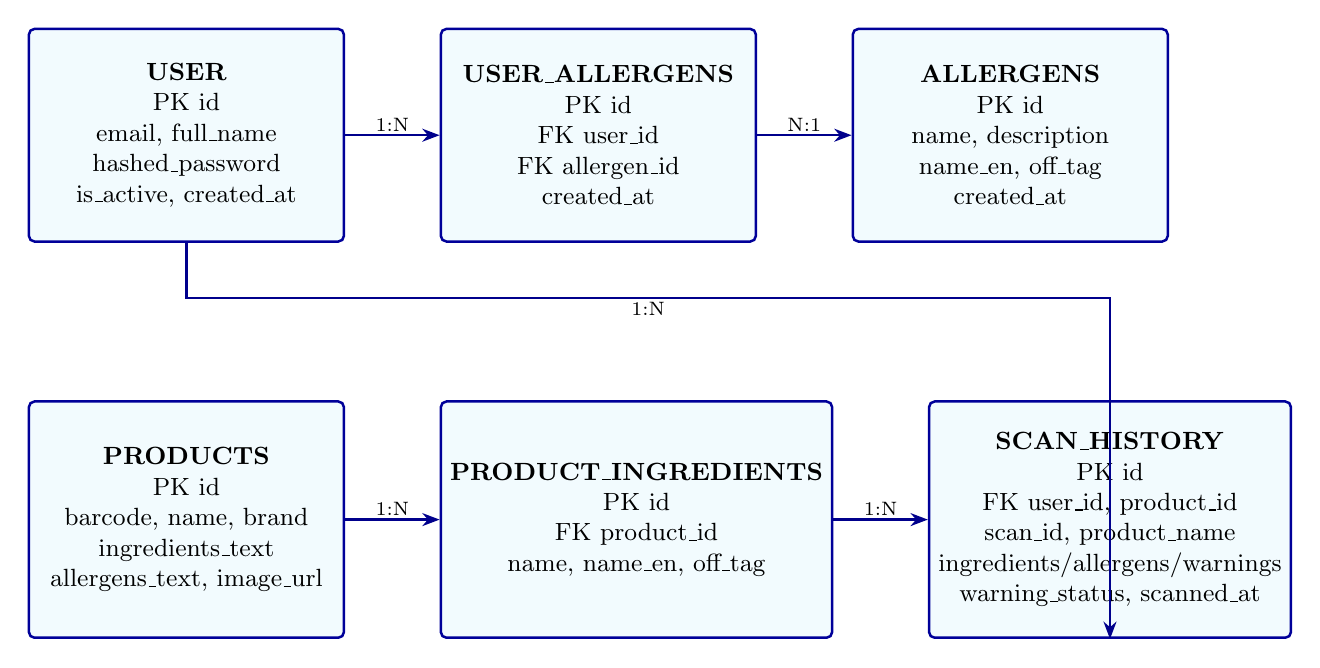
\begin{tikzpicture}[node distance=12mm and 12mm]
\node[awdb,minimum width=4cm,minimum height=27mm] (user) {\textbf{USER}\\PK id\\email, full\_name\\hashed\_password\\is\_active, created\_at};
\node[awdb,right=of user,minimum width=4cm,minimum height=27mm] (ua) {\textbf{USER\_ALLERGENS}\\PK id\\FK user\_id\\FK allergen\_id\\created\_at};
\node[awdb,right=of ua,minimum width=4cm,minimum height=27mm] (all) {\textbf{ALLERGENS}\\PK id\\name, description\\name\_en, off\_tag\\created\_at};
\node[awdb,below=20mm of user,minimum width=4cm,minimum height=30mm] (prod) {\textbf{PRODUCTS}\\PK id\\barcode, name, brand\\ingredients\_text\\allergens\_text, image\_url};
\node[awdb,right=of prod,minimum width=4cm,minimum height=30mm] (pi) {\textbf{PRODUCT\_INGREDIENTS}\\PK id\\FK product\_id\\name, name\_en, off\_tag};
\node[awdb,right=of pi,minimum width=4.2cm,minimum height=30mm] (hist) {\textbf{SCAN\_HISTORY}\\PK id\\FK user\_id, product\_id\\scan\_id, product\_name\\ingredients/allergens/warnings\\warning\_status, scanned\_at};
\draw[awline] (user.east) -- node[awrel,above]{1:N} (ua.west);
\draw[awline] (ua.east) -- node[awrel,above]{N:1} (all.west);
\draw[awline] (prod.east) -- node[awrel,above]{1:N} (pi.west);
\draw[awline] (pi.east) -- node[awrel,above]{1:N} (hist.west);
\draw[awline] (user.south) -- ++(0,-.7) -| node[pos=.25,below,awrel]{1:N} (hist.south);
\end{tikzpicture}}

% =====================================================================
% 3. THÔNG TIN ĐỒ ÁN
% =====================================================================

% Tên báo cáo
\crname{BÁO CÁO ĐỒ ÁN TRÍ TUỆ NHÂN TẠO}

% Tên đề tài
\ctname{
	XÂY DỰNG HỆ THỐNG ĐỌC NHÃN MÁC\\
	VÀ CẢNH BÁO THÀNH PHẦN DỊ ỨNG THỰC PHẨM
}

% Hai sinh viên thực hiện
\cstuname{
	Nguyễn Thị Ngọc Ánh\\
	Huỳnh Đức Bảo
}

% Mã số sinh viên
\cmssv{
	2351220148\\
	2351220048
}

% Lớp
\clopsv{23CT3}

% Hội đồng
\csCouncil{Công nghệ thông tin}

% Giảng viên hướng dẫn
\csSupervise{TS. Đỗ Phúc Hảo}

% Năm học
\cttime{2026--2027}

% Khoa
\csdeptname{KHOA CÔNG NGHỆ THÔNG TIN}

% Địa điểm
\csplace{Đà Nẵng}

% =====================================================================
% 4. BẮT ĐẦU TÀI LIỆU
% =====================================================================

\begin{document}
	
	% =====================================================================
	% 5. TRANG BÌA
	% =====================================================================
	
	\coverpage
	
	% =====================================================================
	% 6. PHẦN ĐẦU BÁO CÁO
	% =====================================================================
	
	\frontmatter
	
	% Thiết lập kiểu trang
	\dauPageStyle
	
	% Lời cam đoan
	% ---------------------------------------------------------------------
%  LỜI CAM ĐOAN
% ---------------------------------------------------------------------
\begin{declaration}

Tôi xin cam đoan đồ án này là công trình do chính tôi thực hiện dưới sự
hướng dẫn của \dauGVHD. Các nội dung nghiên cứu, số liệu và kết quả trình
bày trong đồ án là trung thực và chưa từng được công bố trong bất kỳ công
trình nào khác.

Mọi số liệu, hình ảnh, mã nguồn và kết quả của tác giả khác được sử dụng
trong đồ án đều được trích dẫn nguồn gốc rõ ràng trong phần tài liệu tham
khảo. Toàn bộ phần mềm và thư viện được dùng đều có giấy phép cho phép sử
dụng. Những phần có sử dụng công cụ trí tuệ nhân tạo hỗ trợ đã được nêu rõ
trong báo cáo.

Nếu phát hiện có bất kỳ sự gian lận nào, tôi xin chịu hoàn toàn trách nhiệm
trước Khoa và Nhà trường.

\vspace{1.4em}
\hfill\okyten{\dauSinhVien}{Sinh viên thực hiện}

\end{declaration}

	
	% Lời cảm ơn
	% ---------------------------------------------------------------------
% LỜI CẢM ƠN
% ---------------------------------------------------------------------

\begin{acknowledgments}
	
	Nhóm em xin gửi lời cảm ơn chân thành đến Tiến sĩ Đỗ Phúc Hảo,
	giảng viên hướng dẫn đồ án, đã tận tình hướng dẫn, định hướng
	và đóng góp những ý kiến quý báu trong suốt quá trình thực hiện
	đề tài ``Xây dựng hệ thống đọc nhãn mác và cảnh báo thành phần
	dị ứng thực phẩm''. Những góp ý và sự hỗ trợ của thầy đã giúp
	nhóm em từng bước hoàn thiện nội dung cũng như sản phẩm của đồ án.
	
	Nhóm em cũng xin chân thành cảm ơn quý thầy cô Khoa Công nghệ
	Thông tin, Trường Đại học Kiến trúc Đà Nẵng đã truyền đạt những
	kiến thức và kinh nghiệm quý báu trong suốt quá trình học tập.
	
	Cuối cùng, nhóm em xin cảm ơn gia đình và bạn bè đã luôn quan tâm,
	động viên và tạo điều kiện để nhóm hoàn thành đồ án.
	
	Mặc dù đã cố gắng, nhưng do kiến thức và kinh nghiệm thực tế còn
	hạn chế, đồ án khó tránh khỏi những thiếu sót. Nhóm em rất mong
	nhận được sự góp ý từ quý thầy cô để có thể hoàn thiện đề tài tốt hơn.
	
	\vspace{1.4em}
	\hfill\okyten{\dauSinhVien}{Sinh viên thực hiện}
	
\end{acknowledgments}
	
	% Tóm tắt đồ án
	% ---------------------------------------------------------------------
%  TÓM TẮT
% ---------------------------------------------------------------------
\begin{abstract}

Dị ứng thực phẩm là vấn đề cần được quan tâm vì việc tiếp xúc hoặc tiêu thụ các thành phần gây dị ứng có thể ảnh hưởng đến sức khỏe người dùng. Tuy nhiên, việc kiểm tra nhãn mác và bảng thành phần trên bao bì thực phẩm bằng phương pháp thủ công có thể mất thời gian, đặc biệt khi thông tin được trình bày bằng chữ nhỏ hoặc sử dụng các tên thành phần khó nhận biết. Xuất phát từ thực tế đó, đồ án xây dựng hệ thống đọc nhãn mác và cảnh báo thành phần dị ứng thực phẩm nhằm hỗ trợ người dùng nhận diện thông tin trên bao bì và phát hiện các thành phần có khả năng gây dị ứng.

Hệ thống cho phép người dùng cung cấp hình ảnh nhãn mác thực phẩm, sau đó sử dụng công nghệ nhận dạng ký tự quang học (OCR) để trích xuất văn bản từ hình ảnh. Nội dung thu được được xử lý và phân tích để xác định các thành phần có liên quan đến dị ứng, kết hợp với dữ liệu về chất gây dị ứng và cơ chế hỗ trợ phân tích của trí tuệ nhân tạo. Dựa trên kết quả nhận diện, hệ thống hiển thị thông tin thành phần và đưa ra cảnh báo tương ứng để người dùng có thêm cơ sở tham khảo trước khi lựa chọn thực phẩm. Đồ án hướng đến việc xây dựng một công cụ hỗ trợ tra cứu thuận tiện, góp phần nâng cao nhận thức về an toàn thực phẩm và giảm bớt công sức kiểm tra nhãn mác thủ công. Kết quả của đề tài là cơ sở để tiếp tục hoàn thiện hệ thống về khả năng nhận dạng, độ chính xác khi phân tích thành phần và phạm vi dữ liệu dị ứng được hỗ trợ.

\vspace{0.8em}
\noindent\textbf{Từ khoá:} OCR, nhận dạng ký tự, dị ứng thực phẩm, phân tích thành phần, trí tuệ nhân tạo, cảnh báo dị ứng.


\end{abstract}

	
	% =====================================================================
	% 7. DANH MỤC
	% =====================================================================
	
	% Mục lục
	\tableofcontents
	
	% Danh mục hình ảnh
	\listoffigures
	
	% Danh mục bảng
	\listoftables
	
	% Đồ án không trình bày thuật toán độc lập dạng thuật toán giả mã,
	% vì vậy không tạo Danh mục thuật toán.
	
	% =====================================================================
	% 8. NỘI DUNG CHÍNH CỦA BÁO CÁO
	% =====================================================================
	
	\mainmatter
	
	% Thiết lập kiểu trang cho nội dung chính
	\dauPageStyle
	
	% CHƯƠNG 1: MỞ ĐẦU
	
% ---------------------------------------------------------------------
% CHƯƠNG 1 — MỞ ĐẦU
% ---------------------------------------------------------------------

\chapter{Mở đầu}
\label{ch:modau}

% Không thụt đầu dòng và tạo khoảng cách giữa các đoạn
\setlength{\parindent}{0pt}
\setlength{\parskip}{4pt}

% ---------------------------------------------------------------------
% 1.1. LÝ DO CHỌN ĐỀ TÀI
% ---------------------------------------------------------------------

\section{Lý do chọn đề tài}

Trong cuộc sống hiện nay, thực phẩm đóng vai trò thiết yếu đối với sức khỏe con người. Tuy nhiên, đối với những người có cơ địa dị ứng, việc sử dụng thực phẩm chứa các thành phần không phù hợp có thể gây ra những phản ứng ảnh hưởng đến sức khỏe. Vì vậy, kiểm tra thông tin trên nhãn mác và bảng thành phần trước khi sử dụng là điều cần thiết.

Trên thực tế, thông tin thành phần trên bao bì thường được trình bày bằng chữ nhỏ, sử dụng nhiều thuật ngữ chuyên ngành hoặc các tên gọi khác nhau của cùng một thành phần. Điều này gây khó khăn cho người tiêu dùng trong việc nhận diện các chất có khả năng gây dị ứng. Việc kiểm tra thủ công cũng mất thời gian và có nguy cơ bỏ sót những thông tin quan trọng.

Sự phát triển của trí tuệ nhân tạo và công nghệ xử lý hình ảnh đã tạo điều kiện cho việc tự động hóa quá trình đọc và phân tích nhãn thực phẩm. Thông qua công nghệ nhận dạng ký tự quang học (OCR) kết hợp với các phương pháp xử lý văn bản và trí tuệ nhân tạo, hệ thống có thể trích xuất thông tin, nhận diện thành phần và đối chiếu với dữ liệu dị nguyên để đưa ra cảnh báo.

Xuất phát từ những vấn đề trên, nhóm lựa chọn đề tài “Xây dựng hệ thống đọc nhãn mác và cảnh báo thành phần dị ứng thực phẩm” nhằm xây dựng một ứng dụng web hỗ trợ người dùng kiểm tra thành phần thực phẩm nhanh chóng và thuận tiện. Đồng thời, đề tài giúp nhóm vận dụng kiến thức về trí tuệ nhân tạo, xử lý ảnh, xử lý dữ liệu và phát triển ứng dụng web vào giải quyết một vấn đề thực tiễn.

% ---------------------------------------------------------------------
% 1.2. MỤC TIÊU CỦA ĐỒ ÁN
% ---------------------------------------------------------------------

\section{Mục tiêu của đồ án}

Đồ án hướng đến xây dựng hệ thống hỗ trợ đọc thông tin trên nhãn mác thực phẩm và cảnh báo các thành phần có khả năng gây dị ứng. Các mục tiêu cụ thể bao gồm:

\begin{itemize}[leftmargin=0pt, label={}, itemsep=3pt]
	\item Xây dựng chức năng tiếp nhận hình ảnh nhãn mác hoặc bảng thành phần thực phẩm từ người dùng.
	
	\item Tích hợp công nghệ OCR và trí tuệ nhân tạo để trích xuất, phân tích thông tin từ hình ảnh.
	
	\item Xây dựng cơ chế nhận diện thành phần có khả năng gây dị ứng thông qua xử lý văn bản và đối chiếu dữ liệu dị nguyên.
	
	\item Phát triển chức năng cảnh báo và hiển thị kết quả phân tích để người dùng dễ dàng theo dõi.
	
	\item Xây dựng giao diện web hỗ trợ quét nhãn, quản lý hồ sơ dị ứng và tra cứu lịch sử phân tích.
	
	\item Kiểm thử và đánh giá khả năng nhận diện, phân tích thành phần và độ chính xác của kết quả cảnh báo.
\end{itemize}

Thông qua các mục tiêu trên, nhóm hướng đến xây dựng một hệ thống có khả năng hỗ trợ người dùng trong quá trình kiểm tra và nhận biết các thành phần cần chú ý trên nhãn thực phẩm.

% ---------------------------------------------------------------------
% 1.3. PHẠM VI VÀ ĐỐI TƯỢNG
% ---------------------------------------------------------------------

\section{Phạm vi và đối tượng}

Đối tượng nghiên cứu của đồ án là thông tin thành phần trên nhãn mác thực phẩm, các chất có khả năng gây dị ứng, công nghệ nhận dạng ký tự quang học và việc ứng dụng trí tuệ nhân tạo trong phân tích, cảnh báo dị nguyên.

Phạm vi thực hiện tập trung vào xây dựng hệ thống web cho phép người dùng tải lên hình ảnh nhãn thực phẩm. Hệ thống tiến hành trích xuất văn bản, phân tích thành phần, đối chiếu với dữ liệu dị nguyên và hồ sơ dị ứng của người dùng, sau đó hiển thị kết quả cảnh báo.

Về mặt công nghệ, đồ án tập trung vào xử lý hình ảnh, nhận dạng ký tự, xử lý văn bản, tích hợp trí tuệ nhân tạo, quản lý dữ liệu và phát triển giao diện web.

Hệ thống chỉ có vai trò hỗ trợ nhận diện và cung cấp thông tin tham khảo, không thay thế chuyên gia y tế hoặc đưa ra chẩn đoán dị ứng. Kết quả phụ thuộc vào chất lượng hình ảnh, khả năng nhận dạng và phạm vi dữ liệu được sử dụng. Người dùng cần kiểm tra thông tin trên bao bì thực tế trước khi quyết định sử dụng sản phẩm.

% ---------------------------------------------------------------------
% 1.4. BỐ CỤC BÁO CÁO
% ---------------------------------------------------------------------

\section{Bố cục báo cáo}

Ngoài phần mở đầu, kết luận và tài liệu tham khảo, báo cáo gồm sáu chương:

Chương 1: Mở đầu. Trình bày lý do chọn đề tài, mục tiêu, phạm vi và đối tượng nghiên cứu.

Chương 2: Cơ sở lý thuyết và công nghệ. Giới thiệu các kiến thức nền tảng và công nghệ sử dụng trong hệ thống.

Chương 3: Phân tích và thiết kế hệ thống. Trình bày yêu cầu, kiến trúc, chức năng và quy trình hoạt động của hệ thống.

Chương 4: Cài đặt hệ thống. Mô tả quá trình triển khai các chức năng và xây dựng giao diện ứng dụng.

Chương 5: Kết quả và đánh giá. Trình bày kết quả thực hiện, kiểm thử và đánh giá hệ thống.

Chương 6: Kết luận và hướng phát triển. Tổng kết kết quả đạt được, những hạn chế và đề xuất hướng phát triển trong tương lai.

	
	% CHƯƠNG 2: CƠ SỞ LÝ THUYẾT
	% LƯU Ý: Thêm \usepackage{needspace} vào phần khai báo gói
% trong file do-an.tex, trước \begin{document}.
	% File này dùng gói enumitem (đã có sẵn trong settings hoặc do-an.tex).
	
	% ---------------------------------------------------------------------
	% CHƯƠNG 2 — CƠ SỞ LÝ THUYẾT VÀ CÔNG NGHỆ
	% ---------------------------------------------------------------------
	
	\chapter{Cơ sở lý thuyết và công nghệ}
	\label{ch:cosolythuyet}
	
	% Cấu hình danh sách gạch đầu dòng: thụt vào, dòng đầu thẳng hàng với các dòng sau
	\setlist[itemize,1]{
		label=--,
		leftmargin=1.5cm,
		labelsep=0.5em,
		itemindent=0pt,
		listparindent=0pt,
		parsep=0pt,
		itemsep=4pt,
		topsep=4pt
	}
	
	% ---------------------------------------------------------------------
	% 2.1. KIẾN THỨC NỀN TẢNG
	% ---------------------------------------------------------------------
	
	\Needspace{4\baselineskip}
	\section{Kiến thức nền tảng}
	
	\Needspace{3\baselineskip}
	\subsection{Dị ứng thực phẩm và thành phần gây dị ứng}
	
	Dị ứng thực phẩm là phản ứng của hệ miễn dịch đối với một hoặc nhiều
	thành phần có trong thực phẩm. Tùy thuộc vào cơ địa và mức độ nhạy cảm
	của từng người, phản ứng dị ứng có thể biểu hiện ở nhiều mức độ khác
	nhau. Một số trường hợp có thể xuất hiện các triệu chứng như ngứa,
	phát ban, sưng môi, khó thở hoặc những phản ứng nghiêm trọng hơn.
	
	Trong quá trình lựa chọn thực phẩm, việc kiểm tra thành phần và thông
	tin cảnh báo trên bao bì có ý nghĩa quan trọng đối với người có tiền
	sử dị ứng. Tuy nhiên, thông tin về dị nguyên không phải lúc nào cũng
	được trình bày dưới cùng một cách diễn đạt. Một chất có thể xuất hiện
	dưới tên nguyên liệu, tên khoa học hoặc tên gọi thông dụng khác nhau.
	
	Đối với hệ thống Allergy Warning, dị nguyên được xem xét thông qua
	hai nguồn thông tin chính:
	
	\begin{itemize}
		\item Danh sách thành phần: Các nguyên liệu được ghi trên nhãn sản phẩm. Hệ thống phân tích nội dung này để nhận diện những thành phần có khả năng liên quan đến dị ứng.
		\item Thông tin cảnh báo riêng trên nhãn: Các nội dung do nhà sản xuất công bố, chẳng hạn như ``Contains'' (Chứa) hoặc ``May contain'' (Có thể chứa). Đây là thông tin cảnh báo được trình bày riêng trên bao bì sản phẩm.
	\end{itemize}
	
	Hai nguồn thông tin trên có ý nghĩa khác nhau. Một chất có thể xuất
	hiện trong danh sách thành phần nhưng không được trình bày lại trong
	mục cảnh báo riêng của nhà sản xuất. Vì vậy, không thể chỉ dựa vào
	mục cảnh báo riêng để kết luận sản phẩm không chứa chất gây dị ứng.
	
	Trong phạm vi đồ án, hệ thống sử dụng thông tin thành phần và dữ liệu
	dị nguyên để phân tích sản phẩm. Kết quả được đối chiếu với hồ sơ dị
	ứng mà người dùng đã khai báo nhằm xác định những thành phần cần
	được chú ý.
	
	\Needspace{3\baselineskip}
	\subsection{Nhãn thành phần thực phẩm và thông tin cảnh báo dị nguyên}
	
	Nhãn thực phẩm là nguồn cung cấp thông tin về tên sản phẩm, thương
	hiệu, thành phần nguyên liệu và các nội dung cảnh báo liên quan.
	Thông tin này thường được trình bày dưới dạng văn bản trên bao bì.
	
	Trong quá trình phân tích nhãn, cần phân biệt một số loại thông tin:
	\begin{itemize}
		\item Thành phần nguyên liệu: Liệt kê các chất được sử dụng để sản xuất thực phẩm, ví dụ như bột mì, sữa, dầu thực vật hoặc các loại hạt.
		\item Dị nguyên khai báo riêng: Những chất được nhà sản xuất ghi rõ trong phần cảnh báo dị nguyên trên bao bì.
		\item Cảnh báo có thể chứa vết: Thông tin cảnh báo về khả năng sản phẩm có thể chứa một lượng nhỏ chất gây dị ứng do quá trình sản xuất hoặc đóng gói.
	\end{itemize}

	Việc phân biệt các loại thông tin này giúp hạn chế nhầm lẫn giữa
	thành phần thực tế được liệt kê và nội dung cảnh báo do nhà sản xuất
	công bố.
	
	Đối với Allergy Warning, nội dung trên nhãn được sử dụng làm dữ liệu
	đầu vào cho quá trình nhận dạng và phân tích. Hệ thống cố gắng giữ
	riêng thông tin thành phần, dị nguyên được khai báo và cảnh báo có
	thể chứa vết để kết quả hiển thị rõ ràng hơn.
	
	\Needspace{3\baselineskip}
	\subsection{Nhận dạng và trích xuất văn bản từ hình ảnh}
	
	Nhận dạng ký tự quang học (Optical Character Recognition -- OCR)
	là công nghệ cho phép chuyển đổi chữ viết xuất hiện trong hình ảnh
	thành dữ liệu văn bản có thể xử lý bằng máy tính. Công nghệ này
	được ứng dụng trong việc số hóa tài liệu, nhận dạng thông tin trên
	hóa đơn và trích xuất nội dung từ hình ảnh chứa văn bản.
	
	Đối với bài toán đọc nhãn thực phẩm, quá trình nhận dạng văn bản
	giúp chuyển nội dung được in trên bao bì thành dữ liệu phục vụ
	phân tích. Văn bản sau khi trích xuất có thể chứa tên sản phẩm,
	danh sách thành phần và các thông tin cảnh báo dị nguyên.
	
	Trong đồ án, hệ thống sử dụng Gemini API để hỗ trợ đọc và trích
	xuất thông tin từ hình ảnh nhãn thực phẩm. Thay vì chỉ nhận dạng
	các ký tự riêng lẻ, mô hình AI còn hỗ trợ phân tích nội dung và
	trả về những thông tin có cấu trúc để hệ thống tiếp tục xử lý.
	
	Quá trình xử lý hình ảnh và trích xuất thông tin có thể được mô tả
	qua các bước:
	
	\begin{itemize}
		\item Tiếp nhận hình ảnh nhãn thực phẩm do người dùng tải lên.
		\item Kiểm tra hình ảnh đầu vào và chuẩn bị dữ liệu để xử lý.
		\item Gửi hình ảnh đến dịch vụ Gemini API.
		\item Nhận nội dung văn bản và thông tin sản phẩm được trích xuất.
		\item Kiểm tra dữ liệu trả về và chuyển sang bước phân tích thành phần.
	\end{itemize}
	
	Chất lượng hình ảnh có ảnh hưởng trực tiếp đến kết quả nhận dạng.
	Ảnh bị mờ, thiếu sáng, nghiêng hoặc có kích thước chữ quá nhỏ có
	thể khiến mô hình đọc sai hoặc bỏ sót một số thông tin. Ngoài ra,
	cách bố trí nội dung trên bao bì và ngôn ngữ sử dụng cũng có thể
	ảnh hưởng đến kết quả phân tích.
	
	Do đó, kết quả trích xuất cần được kiểm tra trước khi sử dụng trong
	các bước đối chiếu và tạo cảnh báo.
	
	\Needspace{3\baselineskip}
	\subsection{Tiền xử lý và chuẩn hóa văn bản}
	
	Sau khi trích xuất nội dung từ hình ảnh, dữ liệu văn bản có thể
	chứa khoảng trắng không cần thiết, cách viết hoa và viết thường
	không đồng nhất hoặc những cách diễn đạt khác nhau của cùng một
	thành phần. Vì vậy, tiền xử lý và chuẩn hóa văn bản là bước cần
	thiết để hỗ trợ quá trình phân tích.
	
	Trong hệ thống Allergy Warning, quá trình chuẩn hóa có thể bao gồm:
	
	\begin{itemize}
		\item Loại bỏ khoảng trắng dư thừa và chuẩn hóa định dạng văn bản.
		\item Chuẩn hóa chữ hoa và chữ thường khi thực hiện so sánh.
		\item Tách nội dung danh sách thành phần thành các nguyên liệu riêng biệt khi dữ liệu đầu vào cho phép.
		\item Chuẩn hóa cách biểu diễn tên thành phần để hỗ trợ việc đối chiếu với dữ liệu dị nguyên.
		\item Giữ lại nội dung gốc để phục vụ việc kiểm tra và hiển thị thông tin cho người dùng.
	\end{itemize}
	
	Ví dụ, một thành phần có thể được biểu diễn dưới dạng
	``Whey Powder (Milk)'' hoặc ``whey powder (milk)''. Khi thực hiện
	so sánh, hệ thống có thể chuẩn hóa chữ hoa và chữ thường để hạn chế
	việc bỏ sót do khác biệt về định dạng.
	
	Bên cạnh đó, một số nguyên liệu có thể được gọi bằng nhiều tên
	khác nhau. Vì vậy, quá trình chuẩn hóa cần kết hợp với dữ liệu
	từ khóa hoặc thông tin ánh xạ để hỗ trợ nhận diện thành phần.
	
	Việc chuẩn hóa không đồng nghĩa với việc tự động kết luận một
	nguyên liệu là chất gây dị ứng. Đây là bước chuẩn bị dữ liệu để
	các chức năng phân tích và đối chiếu được thực hiện nhất quán hơn.
	
	\Needspace{3\baselineskip}
	\subsection{Phân tích thành phần và đối chiếu dữ liệu dị nguyên}
	
	Đối chiếu dữ liệu là quá trình so sánh thông tin được trích xuất
	từ nhãn thực phẩm với danh sách dữ liệu dị nguyên đã được lưu trữ.
	Đây là một trong những bước quan trọng của hệ thống Allergy Warning.
	
	Hệ thống sử dụng dữ liệu dị nguyên làm cơ sở tham chiếu để xác
	định những thành phần có khả năng liên quan đến dị ứng. Quá trình
	đối chiếu được thực hiện thông qua các bước cơ bản:
	
	\begin{itemize}
		\item Tiếp nhận danh sách thành phần đã được trích xuất.
		\item Chuẩn hóa nội dung và xác định các tên nguyên liệu.
		\item Đối chiếu tên thành phần với dữ liệu dị nguyên.
		\item Xác định nhóm dị nguyên tương ứng với thành phần được nhận diện.
		\item Tổng hợp kết quả và chuyển sang bước so sánh với hồ sơ dị ứng của người dùng.
	\end{itemize}
	
	Một thành phần có thể được biểu diễn bằng nhiều tên gọi khác nhau.
	Ví dụ, thông tin ``whey powder (milk)'' có thể được nhận diện là
	thành phần liên quan đến sữa. Vì vậy, hệ thống cần xem xét cả tên
	thành phần và các thông tin liên quan thay vì chỉ tìm kiếm một
	từ khóa duy nhất.
	
	Sau khi nhận diện thành phần, hệ thống tiếp tục đối chiếu kết quả
	với hồ sơ dị ứng của người dùng. Nếu dị nguyên được phát hiện
	trùng với dị nguyên mà người dùng đã khai báo, hệ thống hiển thị
	cảnh báo tương ứng.
	
	Cần phân biệt giữa hai kết quả:
	
	\begin{itemize}
		\item Dị nguyên được nhận diện trong sản phẩm: Những nhóm chất có khả năng gây dị ứng được hệ thống xác định từ nội dung thành phần hoặc dữ liệu phân tích.
		\item Dị nguyên trùng với hồ sơ người dùng: Những dị nguyên được nhận diện trong sản phẩm đồng thời nằm trong danh sách dị ứng mà người dùng đã khai báo.
	\end{itemize}
	
	Phương pháp đối chiếu giúp kết quả cảnh báo có căn cứ từ dữ liệu
	được lưu trữ. Tuy nhiên, độ chính xác vẫn phụ thuộc vào chất lượng
	ảnh, nội dung trích xuất, mức độ đầy đủ của dữ liệu dị nguyên và
	cách biểu diễn tên nguyên liệu.
	
	\Needspace{3\baselineskip}
	\subsection{Ứng dụng trí tuệ nhân tạo trong phân tích nhãn thực phẩm}
	
	Trí tuệ nhân tạo (Artificial Intelligence -- AI) là lĩnh vực
	nghiên cứu các phương pháp giúp máy tính thực hiện những nhiệm vụ
	đòi hỏi khả năng phân tích và xử lý thông tin. Trong đồ án
	Allergy Warning, AI được sử dụng để hỗ trợ đọc hình ảnh nhãn
	thực phẩm và phân tích nội dung thành phần.
	
	Hệ thống tích hợp Gemini API để gửi hình ảnh và yêu cầu mô hình
	trích xuất thông tin cần thiết. Kết quả trả về được sử dụng để
	xác định tên sản phẩm, thương hiệu, danh sách thành phần và các
	thông tin cảnh báo dị nguyên khi nội dung trên nhãn cho phép
	nhận diện.
	
	AI có thể hỗ trợ xử lý những trường hợp văn bản có cách diễn đạt
	khác nhau hoặc nội dung được trình bày không đồng nhất. Tuy nhiên,
	kết quả do mô hình tạo ra vẫn có thể chứa thông tin thiếu chính
	xác, bỏ sót thành phần hoặc diễn giải chưa phù hợp với nội dung
	thực tế trên bao bì.
	
	Vì vậy, trong hệ thống cần phân biệt giữa kết quả AI trích xuất
	và kết quả đối chiếu với dữ liệu dị nguyên đã lưu trữ. Hai bước
	này có vai trò bổ trợ cho nhau:
	
	\begin{itemize}
		\item Phân tích bằng AI: Hỗ trợ đọc hình ảnh, trích xuất và diễn giải thông tin trên nhãn thực phẩm.
		\item Đối chiếu dữ liệu: Sử dụng danh sách dị nguyên đã được lưu trữ để kiểm tra các thành phần được nhận diện.
		\item So sánh hồ sơ dị ứng: Kiểm tra những dị nguyên được phát hiện có trùng với thông tin người dùng đã khai báo hay không.
	\end{itemize}
	
	Việc kết hợp AI với dữ liệu dị nguyên giúp hệ thống thực hiện
	quá trình phân tích từ hình ảnh đến kết quả cảnh báo. Tuy nhiên,
	AI không thay thế hoàn toàn việc kiểm tra thông tin trên bao bì
	và không thể bảo đảm phát hiện tất cả các chất gây dị ứng.
	
	Do đó, kết quả của Allergy Warning chỉ có tính chất hỗ trợ
	tham khảo. Người dùng cần kiểm tra lại thông tin trên sản phẩm
	thực tế, đặc biệt trong trường hợp có tiền sử dị ứng nghiêm trọng.
	
	% ---------------------------------------------------------------------
	% 2.2. CÔNG NGHỆ VÀ CÔNG CỤ SỬ DỤNG
	% ---------------------------------------------------------------------
	
	\Needspace{4\baselineskip}
	\section{Công nghệ và công cụ sử dụng}
	
	Để xây dựng hệ thống Allergy Warning, nhóm sử dụng các công nghệ
	phục vụ việc phát triển ứng dụng web, xử lý hình ảnh, phân tích
	thành phần, quản lý dữ liệu và lưu trữ hình ảnh trực tuyến.
	
	Các công nghệ được lựa chọn nhằm đáp ứng những chức năng chính
	của hệ thống, bao gồm quản lý tài khoản, quản lý hồ sơ dị ứng,
	quét nhãn thực phẩm, phân tích dị nguyên và lưu trữ lịch sử quét.
	
	\Needspace{3\baselineskip}
	\subsection{Ngôn ngữ lập trình Python}
	
	Python là ngôn ngữ lập trình bậc cao, có cú pháp tương đối dễ đọc
	và hỗ trợ nhiều thư viện phục vụ phát triển ứng dụng web, xử lý
	dữ liệu và tích hợp các dịch vụ bên ngoài.
	
	Trong đồ án, Python được sử dụng để xây dựng phần xử lý phía máy
	chủ của hệ thống. Ngôn ngữ này đảm nhiệm việc tiếp nhận yêu cầu
	từ giao diện, xử lý dữ liệu đầu vào, gọi dịch vụ AI, thực hiện
	đối chiếu dị nguyên và kết nối cơ sở dữ liệu.
	
	Việc sử dụng Python giúp nhóm tổ chức các chức năng nghiệp vụ
	thành những thành phần riêng biệt, thuận tiện cho quá trình
	phát triển, kiểm thử và bảo trì hệ thống.
	
	\Needspace{3\baselineskip}
	\subsection{Framework Flask}
	
	Flask là một framework web được xây dựng trên nền tảng Python,
	hỗ trợ phát triển ứng dụng web và xây dựng các tuyến xử lý
	yêu cầu từ phía người dùng.
	
	Trong Allergy Warning, Flask được sử dụng để xây dựng máy chủ
	ứng dụng và kết nối các chức năng của hệ thống. Khi người dùng
	thực hiện một thao tác trên giao diện, yêu cầu được gửi đến
	máy chủ Flask để xử lý và trả về kết quả phù hợp.
	
	Các nhiệm vụ chính của Flask trong hệ thống gồm:
	
	\begin{itemize}
		\item Xử lý các yêu cầu đăng ký, đăng nhập và quản lý tài khoản.
		\item Tiếp nhận hình ảnh nhãn thực phẩm do người dùng tải lên.
		\item Gọi dịch vụ Gemini API để hỗ trợ phân tích hình ảnh.
		\item Xử lý dữ liệu thành phần và đối chiếu dị nguyên.
		\item Kết nối cơ sở dữ liệu để lưu trữ và truy xuất thông tin.
		\item Trả kết quả phân tích và lịch sử quét về giao diện web.
	\end{itemize}
	
	Flask đóng vai trò trung tâm trong việc điều phối các thành phần
	xử lý của hệ thống, giúp các chức năng được kết nối thành một
	quy trình thống nhất.
	
	\Needspace{3\baselineskip}
	\subsection{Gemini API}
	
	Gemini API là giao diện lập trình ứng dụng cho phép hệ thống
	tích hợp mô hình trí tuệ nhân tạo Gemini vào ứng dụng của mình.
	Dịch vụ này hỗ trợ tiếp nhận dữ liệu và thực hiện các yêu cầu
	phân tích theo nội dung được gửi đến.
	
	Trong đồ án, Gemini API được sử dụng để hỗ trợ đọc và phân tích
	hình ảnh nhãn thực phẩm. Máy chủ gửi hình ảnh cùng yêu cầu xử lý
	đến dịch vụ AI. Sau đó, hệ thống tiếp nhận kết quả và xử lý
	thông tin trả về.
	
	Các nhiệm vụ chính của Gemini API trong hệ thống gồm:
	
	\begin{itemize}
		\item Hỗ trợ nhận diện nội dung văn bản trên ảnh nhãn thực phẩm.
		\item Trích xuất tên sản phẩm và thương hiệu khi có thông tin.
		\item Trích xuất danh sách thành phần nguyên liệu.
		\item Hỗ trợ nhận diện thông tin dị nguyên được khai báo riêng.
		\item Hỗ trợ nhận diện nội dung cảnh báo có thể chứa vết.
	\end{itemize}
	
	Dữ liệu do Gemini API trả về được máy chủ tiếp nhận và kiểm tra
	trước khi sử dụng cho các bước phân tích tiếp theo. Việc sử dụng
	dịch vụ AI giúp hệ thống xử lý hình ảnh nhãn thực phẩm mà không
	phải xây dựng riêng một mô hình nhận dạng hình ảnh từ đầu.
	
	Tuy nhiên, kết quả phụ thuộc vào chất lượng hình ảnh, nội dung
	yêu cầu gửi đến mô hình và khả năng xử lý của dịch vụ. Vì vậy,
	hệ thống cần có bước kiểm tra dữ liệu trả về và không xem kết
	quả AI là thông tin tuyệt đối chính xác.
	
	\Needspace{3\baselineskip}
	\subsection{TiDB Cloud và cơ sở dữ liệu MySQL}
	
	Cơ sở dữ liệu là thành phần dùng để lưu trữ, quản
	
	% CHƯƠNG 3: PHÂN TÍCH VÀ THIẾT KẾ HỆ THỐNG
	% !TeX root = ../do-an.tex
% CHUONG 3 - PHAN TICH VA THIET KE HE THONG
% Su dung cac hinh PNG trong thu muc assets/

\chapter{Phân tích và thiết kế hệ thống}
\setlength{\parindent}{0pt}

% =========================================================
% 3.1 PHÂN TÍCH BÀI TOÁN
% =========================================================

\Needspace{12\baselineskip}
\section{Phân tích bài toán}

\Needspace{9\baselineskip}
\subsection{Đặt vấn đề}

Thực phẩm là một phần thiết yếu trong đời sống hằng ngày. Tuy nhiên, đối với những người có cơ địa dị ứng thực phẩm, việc lựa chọn sản phẩm cần được thực hiện cẩn thận. Một số thành phần như sữa, trứng, đậu nành, đậu phộng, cá, giáp xác, các loại hạt và lúa mì có thể gây phản ứng dị ứng ở những người nhạy cảm.

Trên bao bì thực phẩm, thông tin thành phần thường được trình bày dưới dạng văn bản với kích thước chữ nhỏ. Một số sản phẩm nhập khẩu sử dụng tiếng Anh, tiếng Pháp, tiếng Đức hoặc ngôn ngữ khác. Điều này gây khó khăn cho người dùng khi đọc và xác định thành phần cần tránh. Bên cạnh đó, hình ảnh nhãn thực phẩm có thể bị mờ, thiếu sáng, nghiêng hoặc chứa nhiều thông tin không liên quan.

Từ thực tế đó, đề tài ``Xây dựng hệ thống đọc nhãn mác và cảnh báo thành phần dị ứng thực phẩm'' được thực hiện nhằm hỗ trợ người dùng trích xuất thông tin từ ảnh nhãn thực phẩm, phân tích thành phần và cảnh báo các dị nguyên có liên quan.

Hệ thống Allergy Warning được xây dựng dưới dạng ứng dụng web. Người dùng có thể đăng ký, đăng nhập, lựa chọn các dị nguyên quan tâm trong hồ sơ cá nhân, tải ảnh nhãn thực phẩm lên để phân tích và xem lại lịch sử quét. Hệ thống sử dụng dữ liệu sản phẩm, danh sách dị nguyên và kết quả phân tích để hỗ trợ người dùng nhận biết những thành phần cần chú ý.

\Needspace{9\baselineskip}
\subsection{Mục tiêu phân tích}

Mục tiêu của quá trình phân tích và thiết kế là xác định các chức năng, dữ liệu và thành phần cần thiết để xây dựng hệ thống.

\textbf{Mục tiêu thứ nhất: Tiếp nhận và đọc ảnh nhãn thực phẩm.}

Hệ thống cho phép người dùng tải ảnh nhãn thực phẩm từ thiết bị. Ảnh được đưa vào quy trình xử lý nhằm trích xuất các thông tin có liên quan đến tên sản phẩm, thương hiệu và danh sách thành phần.

\textbf{Mục tiêu thứ hai: Phân tích thông tin thành phần.}

Thông tin trên ảnh nhãn được Gemini API hỗ trợ nhận diện và trích xuất. Nội dung nhận diện, đặc biệt là tên sản phẩm, thương hiệu, danh sách thành phần và thông tin cảnh báo trên nhãn, được chuẩn hóa trước khi đối chiếu với dữ liệu dị nguyên.

\textbf{Mục tiêu thứ ba: Phân biệt các loại cảnh báo.}

Hệ thống cần phân biệt thành phần có bằng chứng xuất hiện trong danh sách thành phần với thông tin cảnh báo có thể chứa vết dị nguyên trên nhãn. Hai trường hợp này có ý nghĩa khác nhau và không nên được trình bày như cùng một kết luận.

\textbf{Mục tiêu thứ tư: Cá nhân hóa kết quả cảnh báo.}

Người dùng có thể lựa chọn các dị nguyên cần chú ý trong hồ sơ cá nhân. Thông tin này được sử dụng để hỗ trợ việc đối chiếu kết quả phân tích với nhu cầu của từng người dùng.

\textbf{Mục tiêu thứ năm: Lưu trữ và tra cứu thông tin.}

Hệ thống lưu thông tin tài khoản, dữ liệu dị nguyên, sản phẩm, thành phần sản phẩm, hồ sơ dị ứng và lịch sử quét trong cơ sở dữ liệu có khả năng tương thích với MySQL. Trong môi trường phát triển, hệ thống có thể sử dụng MySQL/MariaDB; khi triển khai, dữ liệu được lưu trên TiDB Cloud theo cấu hình kết nối của ứng dụng.

\Needspace{9\baselineskip}
\subsection{Phạm vi của hệ thống}

Hệ thống tập trung vào việc đọc nhãn thực phẩm từ ảnh, trích xuất thông tin, đối chiếu dữ liệu dị nguyên và hiển thị cảnh báo. Dữ liệu sản phẩm có thể được lưu trong cơ sở dữ liệu nội bộ hoặc được thu thập từ nguồn dữ liệu sản phẩm như Open Food Facts.

Kết quả phụ thuộc vào chất lượng ảnh, khả năng trích xuất văn bản, dữ liệu có sẵn và quy tắc đối chiếu. Hệ thống chỉ hỗ trợ người dùng tham khảo thông tin trên nhãn, không thay thế việc đọc nhãn gốc, tư vấn y tế hoặc xác nhận an toàn tuyệt đối của sản phẩm.

% =========================================================
% 3.2 KHẢO SÁT VÀ XÁC ĐỊNH YÊU CẦU
% =========================================================

\Needspace{12\baselineskip}
\section{Khảo sát và xác định yêu cầu hệ thống}

\Needspace{9\baselineskip}
\subsection{Đối tượng sử dụng}

\textbf{Người dùng thông thường:}

Người dùng là đối tượng chính của hệ thống. Người dùng có thể tạo tài khoản, đăng nhập, quản lý hồ sơ dị ứng cá nhân, tải ảnh nhãn thực phẩm để phân tích, xem kết quả và tra cứu lịch sử quét của mình.

\textbf{Quản trị viên:}

Quản trị viên là người được cấp quyền truy cập khu vực quản trị. Thông qua giao diện quản trị, quản trị viên có thể theo dõi Dashboard và thực hiện các thao tác quản lý dữ liệu sản phẩm, dữ liệu liên quan theo những chức năng đã được triển khai trong hệ thống.

\Needspace{9\baselineskip}
\subsection{Yêu cầu chức năng}

\textbf{Chức năng đăng ký tài khoản:}

Cho phép người dùng tạo tài khoản bằng thông tin họ tên, email và mật khẩu. Hệ thống kiểm tra dữ liệu đầu vào và lưu thông tin tài khoản vào cơ sở dữ liệu khi đăng ký hợp lệ.

\textbf{Chức năng đăng nhập:}

Cho phép người dùng nhập email và mật khẩu để xác thực. Khi thông tin hợp lệ, người dùng có thể truy cập các chức năng yêu cầu đăng nhập.

\textbf{Chức năng quản lý hồ sơ cá nhân:}

Hiển thị thông tin tài khoản, bao gồm họ tên và email. Người dùng có thể truy cập khu vực hồ sơ để xem và cập nhật thông tin cá nhân theo chức năng được cung cấp.

\textbf{Chức năng quản lý hồ sơ dị ứng:}

Hệ thống cung cấp danh sách các nhóm dị nguyên như sữa, đậu phộng, đậu nành, trứng, cá, giáp xác, động vật thân mềm, hạt cây, lúa mì, mè, mù tạt, cần tây, đậu lupin và sulfit. Người dùng lựa chọn các mục phù hợp với nhu cầu của mình. Những lựa chọn này được lưu trong bảng \texttt{user\_allergens}.

\textbf{Chức năng tải ảnh nhãn thực phẩm:}

Cho phép người dùng chọn ảnh nhãn thực phẩm từ thiết bị và gửi lên hệ thống. Giao diện hiển thị ảnh hoặc tên ảnh đã chọn và cung cấp thao tác bắt đầu phân tích.

\textbf{Chức năng trích xuất thông tin từ ảnh:}

Hệ thống tiếp nhận ảnh và thực hiện quá trình nhận diện thông tin. Nội dung thu được có thể bao gồm tên sản phẩm, thương hiệu, thành phần và thông tin dị nguyên trên nhãn.

\textbf{Chức năng phân tích thành phần:}

Hệ thống phân tích danh sách thành phần thu được, sau đó đối chiếu với dữ liệu dị nguyên. Những nội dung phù hợp với quy tắc đối chiếu được tổng hợp để phục vụ quá trình cảnh báo.

\textbf{Chức năng cảnh báo dị nguyên:}

Kết quả được chia thành các trường hợp có thành phần liên quan đến dị nguyên và trường hợp có cảnh báo có thể chứa vết dị nguyên. Hệ thống hiển thị tên dị nguyên cùng bằng chứng liên quan để người dùng dễ theo dõi.

\textbf{Chức năng hiển thị kết quả:}

Giao diện kết quả hiển thị tên sản phẩm, thương hiệu, ảnh sản phẩm, danh sách thành phần được nhận diện, các dị nguyên và trạng thái cảnh báo.

\textbf{Chức năng lưu lịch sử quét:}

Hệ thống lưu thông tin mỗi lần quét trong bảng \texttt{scan\_history}, bao gồm mã lần quét, người thực hiện, sản phẩm, ảnh, thành phần, dị nguyên, cảnh báo và thời điểm quét.

\textbf{Chức năng xem lịch sử quét:}

Cho phép người dùng xem lại các sản phẩm đã phân tích và trạng thái cảnh báo của những lần quét trước đó. Người dùng có thể mở chi tiết một lần quét để xem thông tin được lưu.

\textbf{Chức năng quản lý dữ liệu dành cho quản trị viên:}

Khu vực quản trị cung cấp giao diện Dashboard và các màn hình dữ liệu. Tùy theo quyền được cấp, quản trị viên có thể theo dõi thông tin tổng quan, xem dữ liệu sản phẩm, xem chi tiết sản phẩm và kiểm tra các dữ liệu được hệ thống quản lý.

\textbf{Chức năng tra cứu dữ liệu sản phẩm:}

Hệ thống lưu thông tin sản phẩm trong bảng \texttt{products}. Dữ liệu này có thể được dùng để đối chiếu với sản phẩm đã biết khi có thông tin phù hợp, chẳng hạn mã vạch hoặc thông tin nhận diện sản phẩm.

\Needspace{9\baselineskip}
\subsection{Yêu cầu phi chức năng}

\textbf{Tính dễ sử dụng:}

Giao diện được thiết kế theo hướng đơn giản, thống nhất màu sắc và bố cục. Những chức năng chính như quét nhãn, hồ sơ dị ứng và lịch sử quét cần dễ tìm thấy.

\textbf{Tính chính xác:}

Hệ thống cần hạn chế sai sót trong việc nhận diện văn bản và đối chiếu dị nguyên. Độ chính xác thực tế phải được đánh giá thông qua kiểm thử với các ảnh nhãn khác nhau.

\textbf{Tính bảo mật:}

Thông tin tài khoản và lịch sử quét cần được bảo vệ. Mật khẩu cần được lưu dưới dạng giá trị băm thay vì văn bản thuần. Các chức năng liên quan đến hồ sơ cá nhân cần kiểm soát quyền truy cập phù hợp.

\textbf{Tính nhất quán của dữ liệu:}

Thông tin người dùng, sản phẩm, thành phần và dị nguyên cần được tổ chức thống nhất. Các khóa chính, khóa ngoại và ràng buộc duy nhất giúp hạn chế dữ liệu trùng lặp và sai lệch.

\textbf{Khả năng mở rộng:}

Cơ sở dữ liệu cần hỗ trợ bổ sung sản phẩm, thành phần và nhóm dị nguyên khi có dữ liệu mới.

\textbf{Khả năng bảo trì:}

Các chức năng giao diện, xử lý ảnh, phân tích thành phần và truy xuất dữ liệu nên được tổ chức rõ ràng để thuận tiện cho việc kiểm tra, sửa lỗi và nâng cấp.

\textbf{Tính minh bạch:}

Kết quả cần trình bày bằng chứng liên quan đến cảnh báo. Việc không phát hiện dị nguyên không đồng nghĩa với việc sản phẩm chắc chắn an toàn đối với mọi người.

% =========================================================
% 3.3 PHÂN TÍCH VÀ MÔ HÌNH HÓA USE CASE
% =========================================================

\Needspace{12\baselineskip}
\section{Phân tích và mô hình hóa Use Case}

\Needspace{9\baselineskip}
\subsection{Xác định tác nhân}

Dựa trên các yêu cầu chức năng đã xác định, hệ thống Allergy Warning có hai nhóm tác nhân chính là người dùng và quản trị viên.

\begin{itemize}
	\item \textbf{Người dùng:} Có thể đăng ký tài khoản, đăng nhập, xem hồ sơ cá nhân, lựa chọn các nhóm dị nguyên cần chú ý, tải ảnh nhãn thực phẩm để phân tích, xem kết quả và tra cứu lịch sử quét.
	\item \textbf{Quản trị viên:} Truy cập khu vực quản trị để theo dõi Dashboard và quản lý, tra cứu dữ liệu sản phẩm theo quyền được cấp.
\end{itemize}

\Needspace{9\baselineskip}
\subsection{Sơ đồ Use Case tổng quát}

Sơ đồ Use Case tổng quát mô tả các chức năng chính mà người dùng có thể thực hiện khi tương tác với hệ thống Allergy Warning. Các chức năng được chia thành nhóm tài khoản, hồ sơ dị ứng, quét nhãn, kết quả phân tích và tra cứu lịch sử.

\begin{figure}[H]
	\centering
	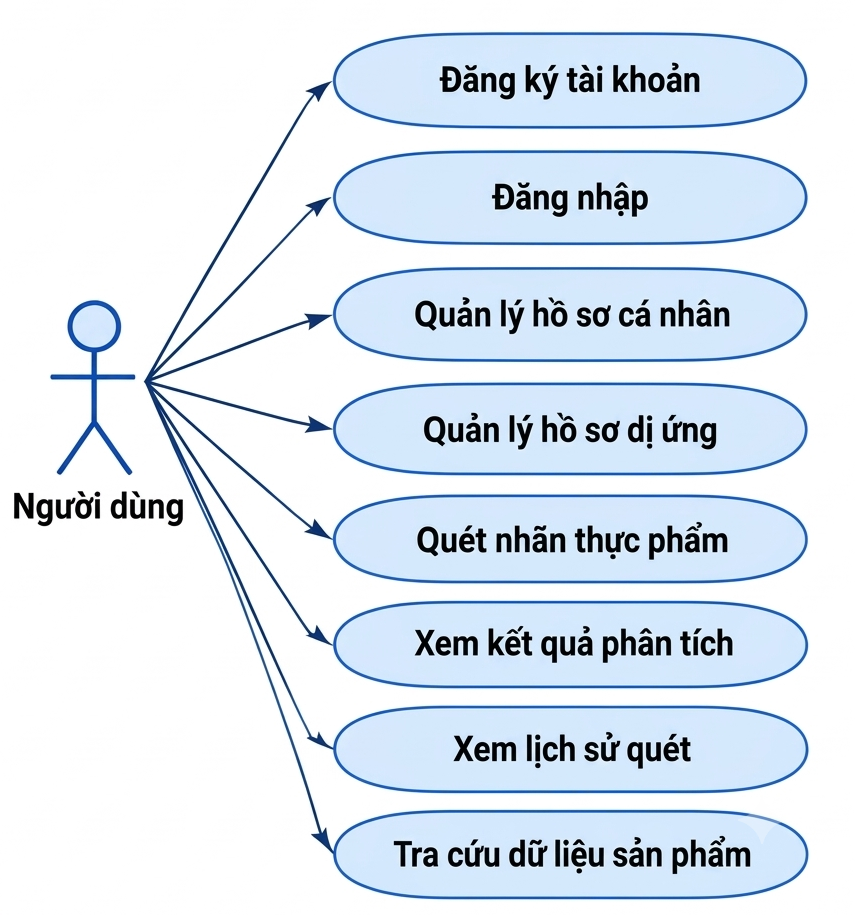
\includegraphics[width=0.82\textwidth,height=0.70\textheight,keepaspectratio]{assets/01_usecase_tongquat.png}
	\caption{Sơ đồ Use Case tổng quát của hệ thống Allergy Warning}
	\label{fig:usecase-tongquat}
\end{figure}

Sơ đồ cho thấy người dùng tương tác với tám nhóm chức năng chính: đăng ký, đăng nhập, quản lý hồ sơ cá nhân, quản lý hồ sơ dị ứng, quét nhãn, xem kết quả, xem lịch sử và tra cứu dữ liệu sản phẩm.


\Needspace{9\baselineskip}
\subsection{Sơ đồ Use Case phân rã chức năng tài khoản}

Nhóm chức năng tài khoản cho phép người dùng tạo tài khoản và xác thực trước khi sử dụng những chức năng yêu cầu đăng nhập. Quá trình đăng ký bao gồm nhập thông tin, kiểm tra dữ liệu và tạo tài khoản. Quá trình đăng nhập bao gồm nhập thông tin xác thực và kiểm tra trạng thái tài khoản.

\begin{figure}[H]
	\centering
	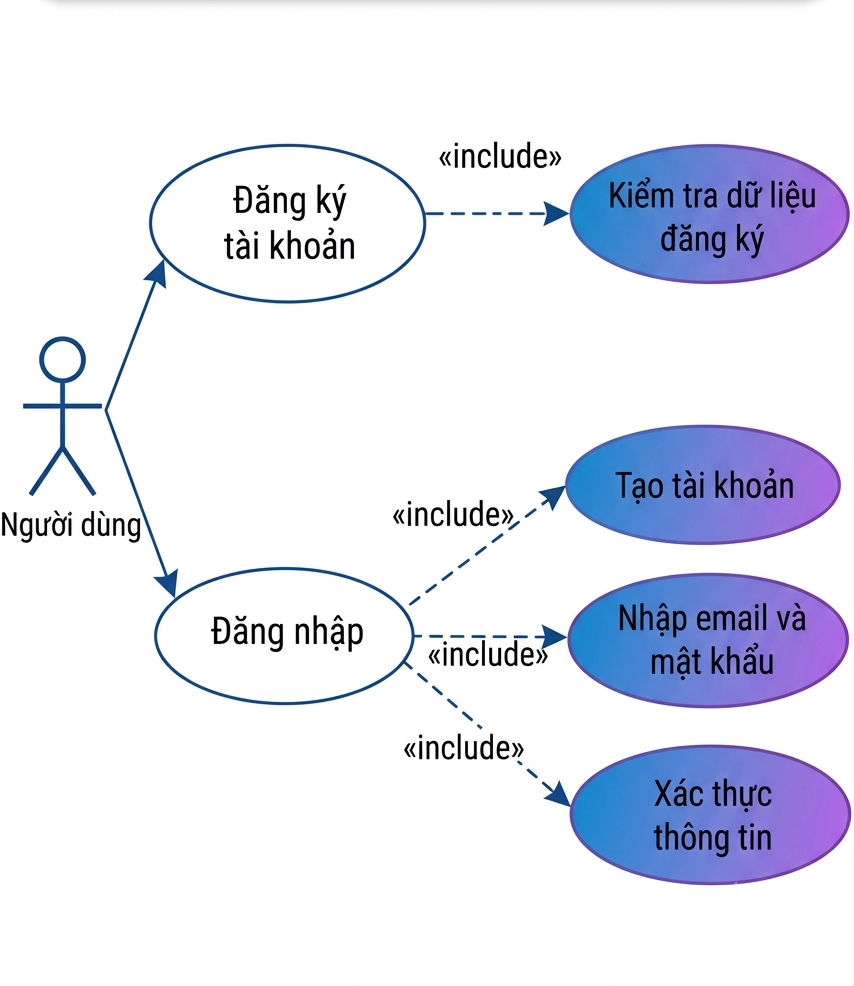
\includegraphics[width=0.82\textwidth,height=0.70\textheight,keepaspectratio]{assets/02_usecase_taikhoan.png}
	\caption{Sơ đồ Use Case phân rã chức năng quản lý tài khoản}
	\label{fig:usecase-taikhoan}
\end{figure}

Sơ đồ phân rã hai chức năng tài khoản. Đăng ký bao gồm kiểm tra dữ liệu trước khi tạo tài khoản; đăng nhập bao gồm nhập email, mật khẩu và xác thực thông tin để cấp quyền truy cập.


\Needspace{9\baselineskip}
\subsection{Sơ đồ Use Case phân rã chức năng quản lý hồ sơ dị ứng}

Chức năng hồ sơ dị ứng cho phép người dùng xem thông tin cá nhân và lựa chọn những nhóm dị nguyên cần chú ý. Danh sách dị nguyên được lấy từ dữ liệu hệ thống. Các lựa chọn của người dùng được liên kết với tài khoản thông qua bảng \texttt{user\_allergens}.

\begin{figure}[H]
	\centering
	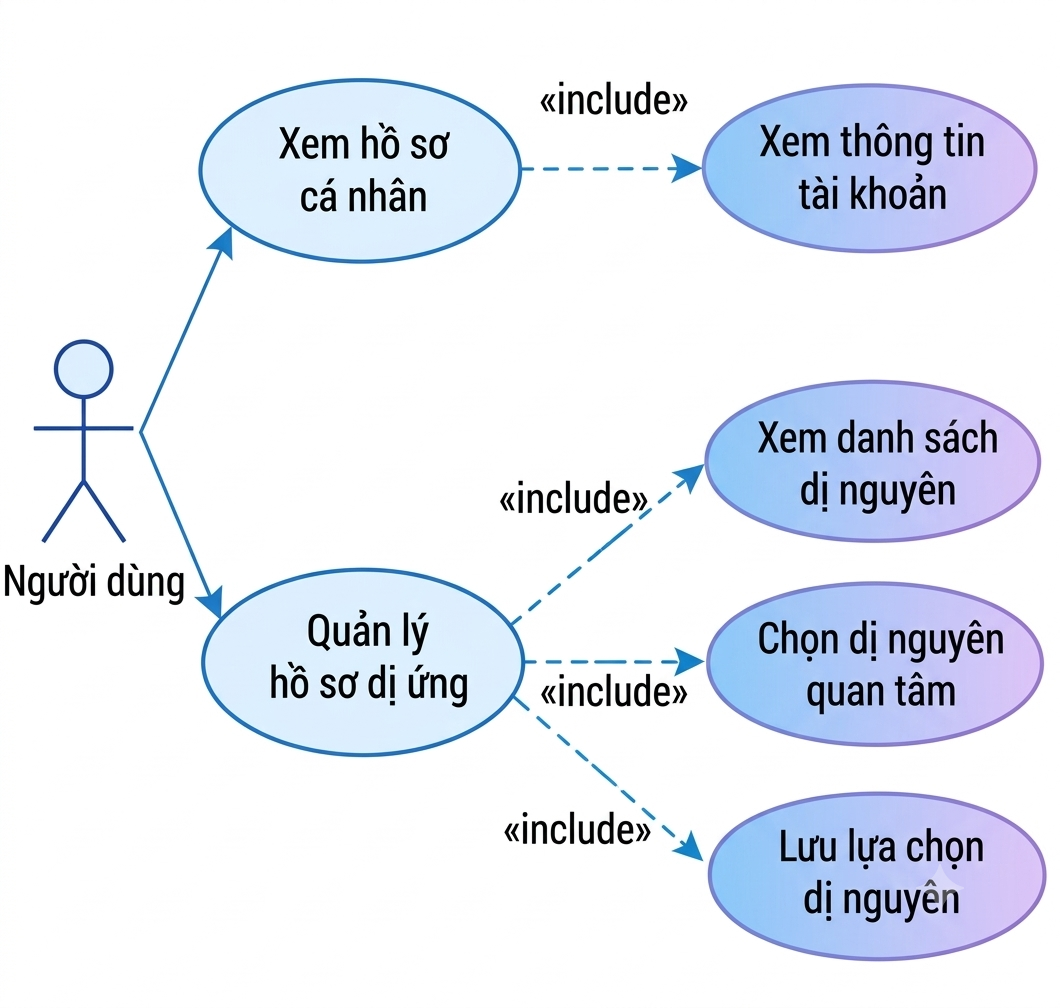
\includegraphics[width=0.82\textwidth,height=0.70\textheight,keepaspectratio]{assets/03_usecase_hoso.png}
	\caption{Sơ đồ Use Case phân rã chức năng quản lý hồ sơ dị ứng}
	\label{fig:usecase-hoso-diung}
\end{figure}

Sơ đồ thể hiện người dùng xem hồ sơ cá nhân và quản lý hồ sơ dị ứng. Với hồ sơ dị ứng, người dùng xem danh sách, chọn các dị nguyên quan tâm và lưu lựa chọn để sử dụng trong những lần phân tích tiếp theo.


\Needspace{9\baselineskip}
\subsection{Sơ đồ Use Case phân rã chức năng quét nhãn thực phẩm}

Quét nhãn thực phẩm là chức năng trọng tâm của hệ thống. Người dùng cung cấp ảnh nhãn, hệ thống kiểm tra ảnh và gửi ảnh đến Gemini API để nhận diện, trích xuất thông tin. Nội dung nhận diện được chuẩn hóa, phân tích thành phần và đối chiếu với dữ liệu dị nguyên. Kết quả được phân loại thành các trường hợp có dị nguyên trong thành phần, có cảnh báo khả năng chứa vết dị nguyên hoặc chưa đủ dữ liệu xác định.

\begin{figure}[H]
	\centering
	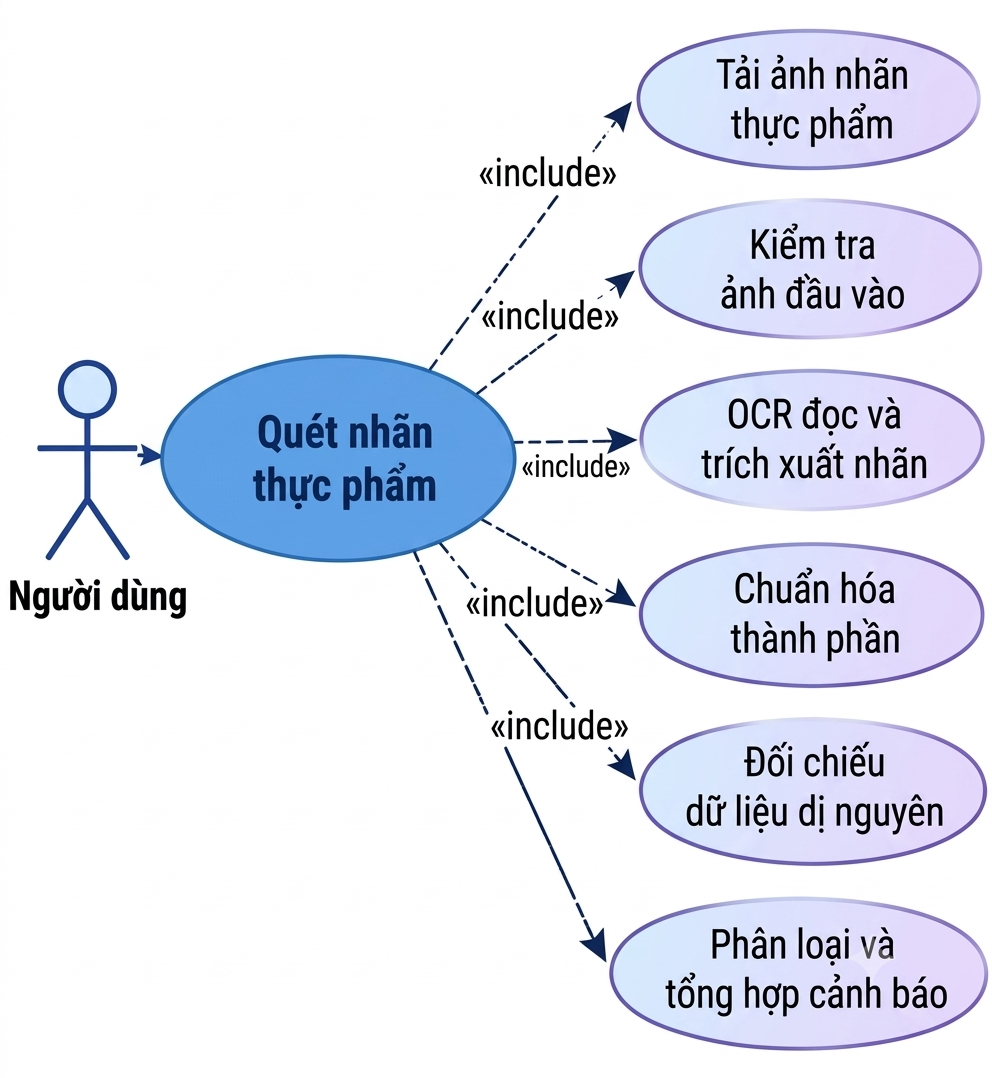
\includegraphics[width=0.92\textwidth,height=0.70\textheight,keepaspectratio]{assets/04_usecase_quetnhan.png}
	\caption{Sơ đồ Use Case phân rã chức năng quét nhãn thực phẩm}
	\label{fig:usecase-quet-nhan}
\end{figure}

Sơ đồ mô tả chức năng quét nhãn và các bước được hệ thống thực hiện: tải ảnh, kiểm tra ảnh đầu vào, dùng OCR/AI trích xuất nội dung, chuẩn hóa thành phần, đối chiếu dữ liệu dị nguyên và tổng hợp cảnh báo.


\Needspace{9\baselineskip}
\subsection{Sơ đồ Use Case phân rã chức năng kết quả và lịch sử}

Sau khi quá trình phân tích hoàn tất, người dùng có thể xem kết quả, theo dõi bằng chứng liên quan đến dị nguyên và tra cứu lại những lần quét trước đó. Dữ liệu lịch sử được truy xuất theo tài khoản đang đăng nhập.

\begin{figure}[H]
	\centering
	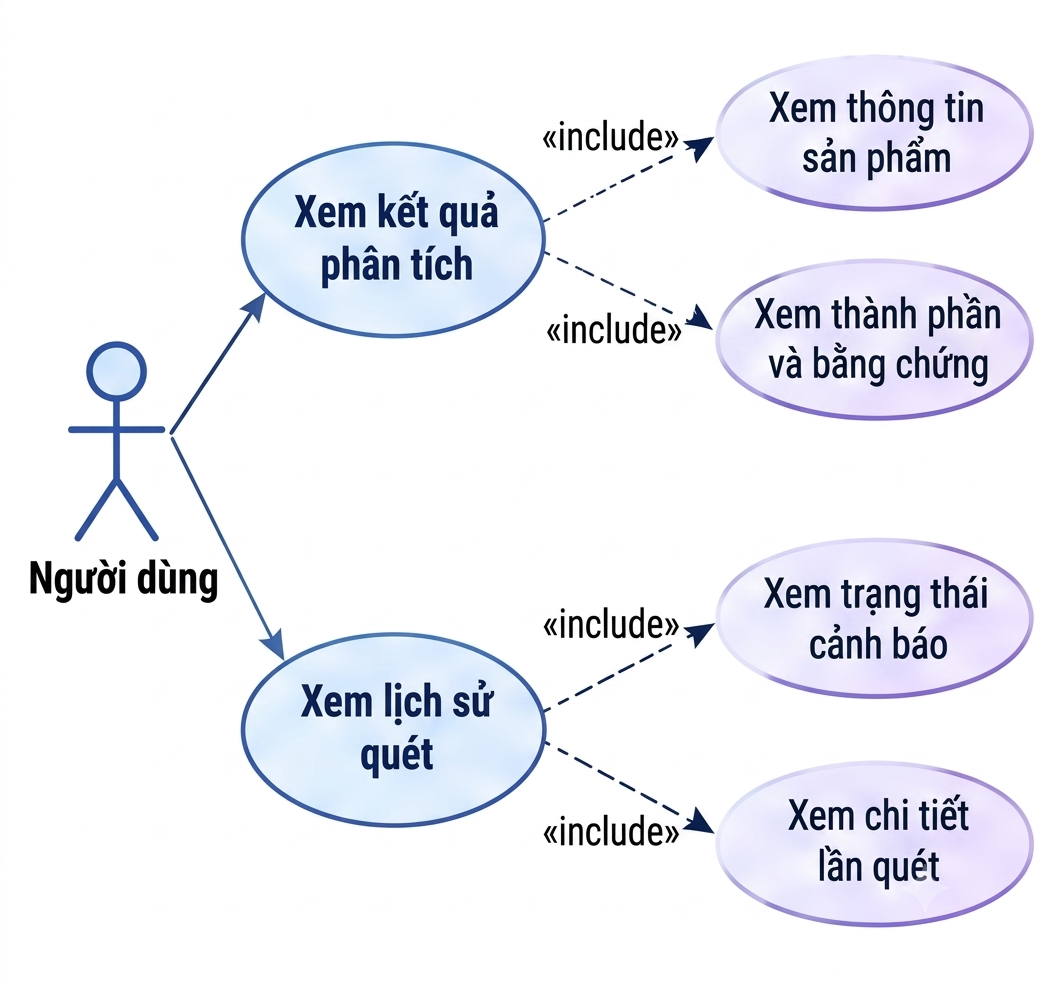
\includegraphics[width=0.82\textwidth,height=0.70\textheight,keepaspectratio]{assets/05_usecase_ketqua.png}
	\caption{Sơ đồ Use Case phân rã chức năng kết quả và lịch sử quét}
	\label{fig:usecase-ketqua-lichsu}
\end{figure}

Sơ đồ thể hiện hai chức năng sau khi quét. Người dùng có thể xem thông tin sản phẩm, thành phần và bằng chứng cảnh báo; đồng thời tra cứu trạng thái và chi tiết của những lần quét đã lưu.


\Needspace{9\baselineskip}
\subsection{Đặc tả các Use Case chính}

Dựa trên các sơ đồ Use Case, những chức năng chính của hệ thống được mô tả tóm tắt trong Bảng~\ref{tab:usecase-description}.

\begin{table}[H]
	\centering
	\caption{Đặc tả các Use Case chính của hệ thống}
	\label{tab:usecase-description}
	\small
	\begin{tabularx}{\textwidth}{|c|l|X|}
		\hline
		\textbf{Mã UC} & \textbf{Tên Use Case} & \textbf{Mô tả chức năng} \\
		\hline
		UC01 & Đăng ký tài khoản & Người dùng nhập họ tên, email và mật khẩu để tạo tài khoản mới. \\
		\hline
		UC02 & Đăng nhập & Người dùng nhập email và mật khẩu để xác thực và truy cập hệ thống. \\
		\hline
		UC03 & Quản lý hồ sơ cá nhân & Người dùng xem thông tin tài khoản của mình. \\
		\hline
		UC04 & Quản lý hồ sơ dị ứng & Người dùng lựa chọn và cập nhật các nhóm dị nguyên cần chú ý. \\
		\hline
		UC05 & Quét nhãn thực phẩm & Người dùng tải ảnh nhãn thực phẩm lên để hệ thống phân tích. \\
		\hline
		UC06 & Xem kết quả phân tích & Người dùng xem thông tin sản phẩm, thành phần và cảnh báo dị nguyên. \\
		\hline
		UC07 & Xem lịch sử quét & Người dùng xem lại những lần quét và kết quả trước đó. \\
		\hline
		UC08 & Quản lý dữ liệu sản phẩm & Quản trị viên tra cứu và quản lý dữ liệu sản phẩm theo quyền được cấp. \\
		\hline
	\end{tabularx}
\end{table}

\Needspace{7\baselineskip}
\subsubsection{Đặc tả Use Case đăng ký tài khoản}

\textbf{Tác nhân:} Người dùng.

\textbf{Mục đích:} Tạo tài khoản mới để sử dụng các chức năng của hệ thống.

\textbf{Điều kiện tiên quyết:} Người dùng chưa có tài khoản sử dụng email đăng ký.

\textbf{Luồng sự kiện chính:}
\begin{enumerate}
	\item Người dùng truy cập trang đăng ký.
	\item Người dùng nhập họ tên, email, mật khẩu và xác nhận mật khẩu.
	\item Hệ thống kiểm tra các trường dữ liệu bắt buộc.
	\item Hệ thống kiểm tra email đã tồn tại hay chưa.
	\item Nếu dữ liệu hợp lệ, hệ thống băm mật khẩu và lưu tài khoản.
	\item Hệ thống thông báo đăng ký thành công.
\end{enumerate}

\textbf{Luồng ngoại lệ:}
\begin{itemize}
	\item Thiếu thông tin: Hệ thống yêu cầu nhập đầy đủ.
	\item Email đã tồn tại: Hệ thống thông báo email đã được sử dụng.
	\item Mật khẩu xác nhận không khớp: Hệ thống yêu cầu kiểm tra lại.
\end{itemize}

\textbf{Điều kiện hậu:} Tài khoản mới được lưu trong cơ sở dữ liệu khi đăng ký thành công.

\Needspace{7\baselineskip}
\subsubsection{Đặc tả Use Case đăng nhập}

\textbf{Tác nhân:} Người dùng.

\textbf{Mục đích:} Xác thực tài khoản để truy cập các chức năng yêu cầu đăng nhập.

\textbf{Điều kiện tiên quyết:} Người dùng đã có tài khoản trong hệ thống.

\textbf{Luồng sự kiện chính:}
\begin{enumerate}
	\item Người dùng mở trang đăng nhập.
	\item Người dùng nhập email và mật khẩu.
	\item Hệ thống kiểm tra thông tin xác thực.
	\item Hệ thống kiểm tra trạng thái hoạt động của tài khoản.
	\item Nếu thông tin hợp lệ, người dùng được chuyển đến trang chính.
\end{enumerate}

\textbf{Luồng ngoại lệ:}
\begin{itemize}
	\item Email hoặc mật khẩu không chính xác: Hệ thống thông báo đăng nhập thất bại.
	\item Tài khoản không hoạt động: Hệ thống từ chối truy cập.
\end{itemize}

\textbf{Điều kiện hậu:} Người dùng được xác thực và có thể truy cập các chức năng phù hợp.

\Needspace{7\baselineskip}
\subsubsection{Đặc tả Use Case quản lý hồ sơ dị ứng}

\textbf{Tác nhân:} Người dùng.

\textbf{Mục đích:} Lưu các nhóm dị nguyên mà người dùng muốn hệ thống chú ý.

\textbf{Điều kiện tiên quyết:} Người dùng đã đăng nhập.

\textbf{Luồng sự kiện chính:}
\begin{enumerate}
	\item Người dùng truy cập trang hồ sơ cá nhân.
	\item Hệ thống hiển thị danh sách các nhóm dị nguyên.
	\item Người dùng lựa chọn hoặc bỏ lựa chọn dị nguyên.
	\item Người dùng xác nhận cập nhật.
	\item Hệ thống lưu lựa chọn vào bảng \texttt{user\_allergens}.
	\item Hệ thống thông báo cập nhật thành công.
\end{enumerate}

\textbf{Luồng ngoại lệ:}
\begin{itemize}
	\item Dữ liệu cập nhật không hợp lệ: Hệ thống yêu cầu kiểm tra lại.
	\item Lỗi lưu dữ liệu: Hệ thống thông báo chưa thể cập nhật hồ sơ.
\end{itemize}

\textbf{Điều kiện hậu:} Hồ sơ dị ứng được cập nhật để sử dụng trong những lần phân tích tiếp theo.

\Needspace{7\baselineskip}
\subsubsection{Đặc tả Use Case quét nhãn thực phẩm}

\textbf{Tác nhân:} Người dùng.

\textbf{Mục đích:} Trích xuất thông tin trên nhãn thực phẩm, đối chiếu thành phần và nhận cảnh báo về các dị nguyên liên quan.

\textbf{Điều kiện tiên quyết:}
\begin{itemize}
	\item Người dùng đã đăng nhập.
	\item Người dùng có ảnh nhãn thực phẩm cần phân tích.
\end{itemize}

\textbf{Luồng sự kiện chính:}
\begin{enumerate}
	\item Người dùng truy cập chức năng quét nhãn.
	\item Người dùng chọn ảnh nhãn từ thiết bị.
	\item Hệ thống tiếp nhận và kiểm tra ảnh đầu vào.
	\item Hệ thống nhận diện và trích xuất thông tin từ ảnh.
	\item Nội dung nhận diện được chuẩn hóa.
	\item Hệ thống đối chiếu thành phần với dữ liệu dị nguyên.
	\item Hệ thống phân loại các trường hợp có dị nguyên trong thành phần, cảnh báo có thể chứa vết dị nguyên hoặc chưa đủ dữ liệu xác định.
	\item Hệ thống tổng hợp thông tin sản phẩm và kết quả cảnh báo.
	\item Kết quả được lưu vào lịch sử quét.
	\item Hệ thống hiển thị kết quả cho người dùng.
\end{enumerate}

\textbf{Luồng ngoại lệ:}
\begin{itemize}
	\item Ảnh không hợp lệ: Hệ thống yêu cầu chọn lại ảnh.
	\item Không nhận diện được nội dung: Hệ thống thông báo không đủ dữ liệu.
	\item Lỗi phân tích: Hệ thống thông báo lỗi và cho phép thực hiện lại.
	\item Không xác định được sản phẩm: Hệ thống vẫn có thể hiển thị kết quả dựa trên nội dung nhận diện được nếu dữ liệu đáp ứng yêu cầu xử lý.
\end{itemize}

\textbf{Điều kiện hậu:} Kết quả được hiển thị và lưu vào lịch sử quét khi quá trình xử lý hoàn thành thành công.

\Needspace{7\baselineskip}
\subsubsection{Đặc tả Use Case xem lịch sử quét}

\textbf{Tác nhân:} Người dùng.

\textbf{Mục đích:} Tra cứu lại những sản phẩm đã được phân tích trước đó.

\textbf{Điều kiện tiên quyết:} Người dùng đã đăng nhập.

\textbf{Luồng sự kiện chính:}
\begin{enumerate}
	\item Người dùng truy cập chức năng lịch sử quét.
	\item Hệ thống xác định tài khoản đang đăng nhập.
	\item Hệ thống truy xuất bản ghi tương ứng trong bảng \texttt{scan\_history}.
	\item Hệ thống hiển thị tên sản phẩm, thời điểm quét và trạng thái cảnh báo.
	\item Người dùng chọn bản ghi để xem chi tiết nếu giao diện hỗ trợ.
\end{enumerate}

\textbf{Luồng ngoại lệ:}
\begin{itemize}
	\item Chưa có lịch sử: Hệ thống thông báo chưa có dữ liệu.
	\item Lỗi truy xuất: Hệ thống thông báo không thể tải lịch sử.
\end{itemize}

\textbf{Điều kiện hậu:} Người dùng xem được các bản ghi lịch sử thuộc tài khoản của mình.

% =========================================================
% 3.4 KIẾN TRÚC HỆ THỐNG
% =========================================================

\Needspace{12\baselineskip}
\section{Thiết kế kiến trúc hệ thống}

\Needspace{9\baselineskip}
\subsection{Kiến trúc tổng thể}

Hệ thống Allergy Warning được tổ chức thành các thành phần chính gồm giao diện web, xử lý nghiệp vụ phía máy chủ, thành phần nhận diện và phân tích nội dung nhãn, cùng cơ sở dữ liệu. Các thành phần phối hợp để tiếp nhận ảnh, xử lý thông tin và trả kết quả cảnh báo cho người dùng.

\begin{figure}[H]
	\centering
	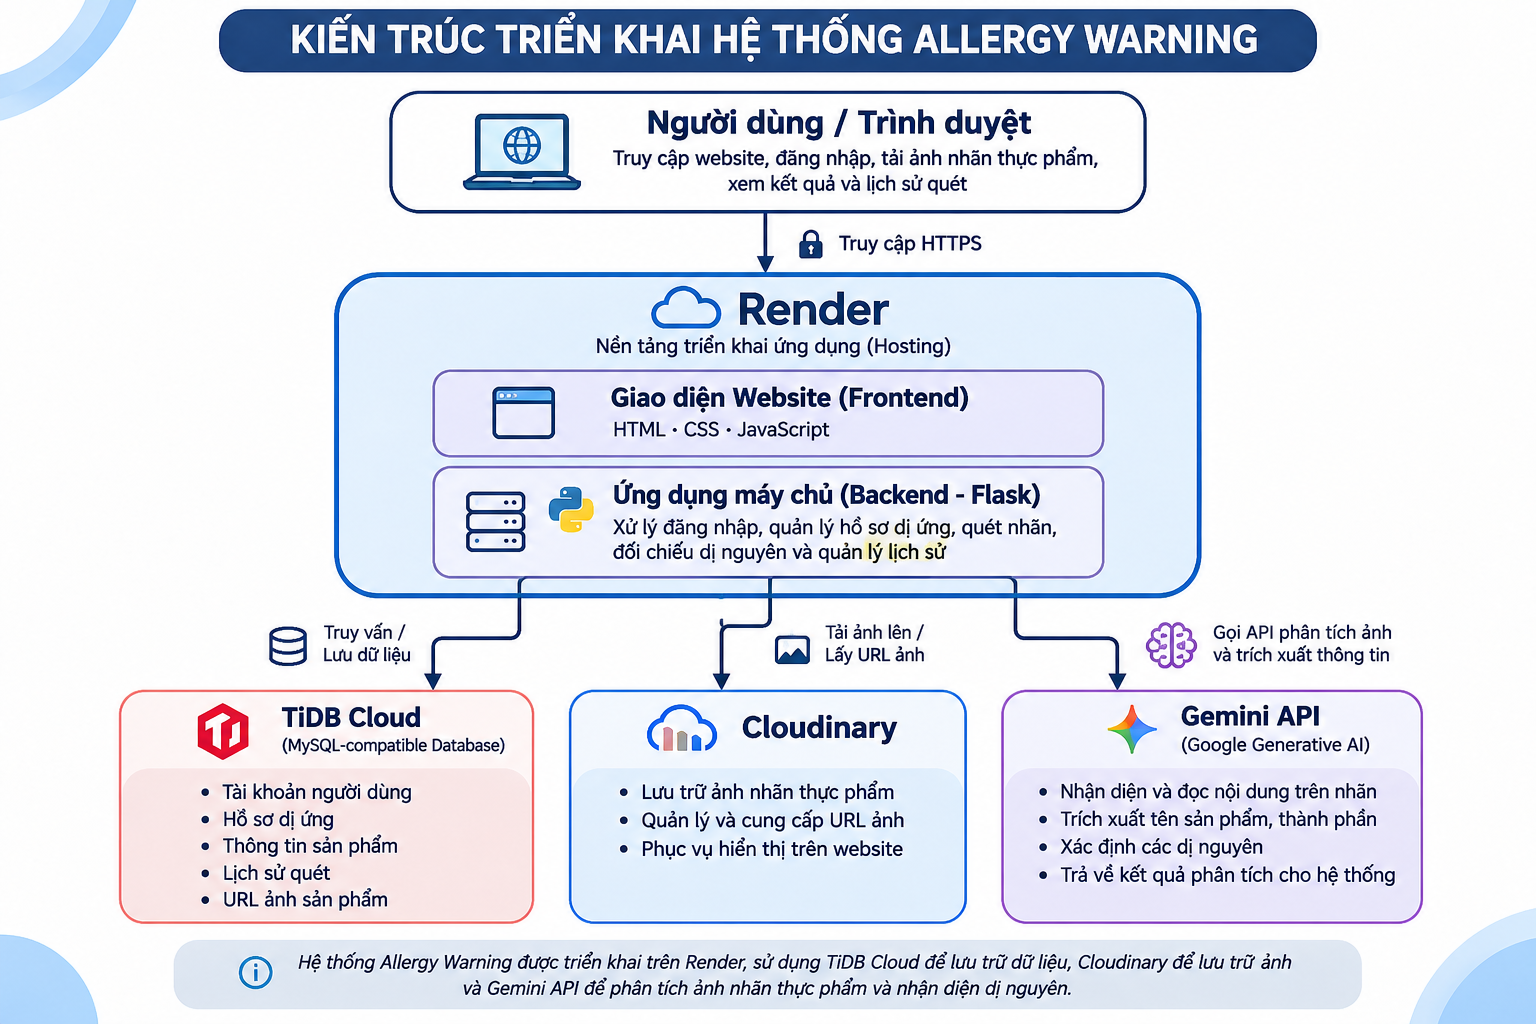
\includegraphics[width=0.95\textwidth,height=0.68\textheight,keepaspectratio]{assets/06_kien_truc_tong_the.png}
	\caption{Kiến trúc tổng thể của hệ thống Allergy Warning}
	\label{fig:kien-truc-he-thong}
\end{figure}

Sơ đồ thể hiện người dùng truy cập website qua HTTPS; ứng dụng Flask được triển khai trên Render, xử lý yêu cầu từ trình duyệt và kết nối các dịch vụ. TiDB Cloud lưu dữ liệu quan hệ, Cloudinary lưu ảnh và cung cấp URL, còn Gemini API phân tích ảnh nhãn và trích xuất thông tin.


\Needspace{9\baselineskip}
\subsection{Sơ đồ kiến trúc xử lý ảnh và phân tích dị nguyên}

Bên cạnh kiến trúc tổng thể, quy trình xử lý nhãn thực phẩm được chia thành các công đoạn. Ảnh đầu vào được tiếp nhận và kiểm tra tính hợp lệ, sau đó được gửi đến Gemini API để nhận diện nội dung hình ảnh và trích xuất thông tin dạng văn bản. Ứng dụng tiếp tục chuẩn hóa kết quả, phân tích tên sản phẩm, thương hiệu, thành phần và các cụm từ cảnh báo. Những thông tin thu được được đối chiếu với dữ liệu dị nguyên để tổng hợp cảnh báo và lưu trữ.

\begin{figure}[H]
	\centering
	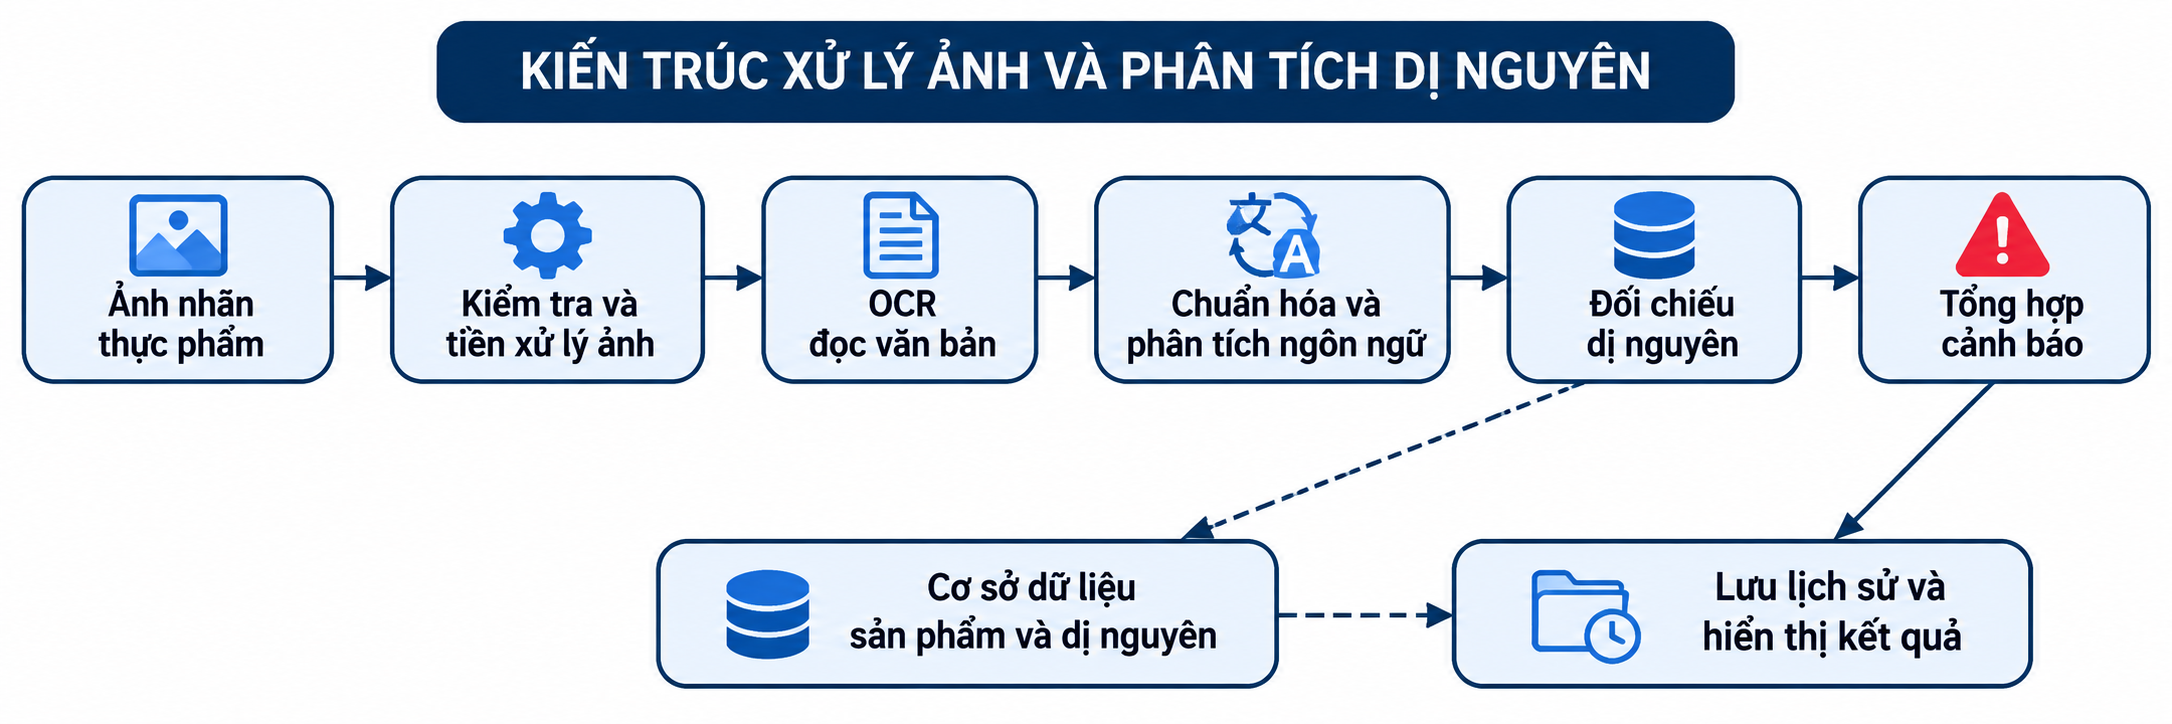
\includegraphics[width=0.95\textwidth,height=0.68\textheight,keepaspectratio]{assets/07_kien_truc_xu_ly.png}
	\caption{Kiến trúc xử lý ảnh và phân tích dị nguyên}
	\label{fig:kien-truc-xu-ly}
\end{figure}

Sơ đồ mô tả chuỗi xử lý ảnh: tiếp nhận ảnh, kiểm tra và tiền xử lý, OCR/AI đọc nội dung, chuẩn hóa ngôn ngữ, đối chiếu dị nguyên, tổng hợp cảnh báo, sau đó lưu lịch sử và hiển thị kết quả.


\Needspace{9\baselineskip}
\subsection{Giao diện web}

Giao diện web là nơi người dùng thực hiện các thao tác với hệ thống. Các trang chính được thể hiện qua những màn hình đăng nhập, đăng ký, Dashboard, quét nhãn, hồ sơ cá nhân, lịch sử quét và kết quả phân tích.

Giao diện sử dụng màu xanh lá làm màu nhấn, nền sáng và các thẻ nội dung riêng biệt. Cách trình bày này giúp phân chia rõ khu vực tải ảnh, danh sách dị nguyên và kết quả cảnh báo.

\Needspace{9\baselineskip}
\subsection{Thành phần xử lý nghiệp vụ}

Thành phần xử lý nghiệp vụ phía máy chủ được xây dựng bằng Flask. Thành phần này tiếp nhận yêu cầu từ giao diện web, kiểm tra dữ liệu đầu vào, điều phối quá trình phân tích ảnh, xử lý kết quả trả về, quản lý tài khoản, truy xuất dữ liệu sản phẩm và lưu lịch sử quét. Máy chủ cũng thực hiện việc kết nối đến các dịch vụ bên ngoài theo cấu hình của hệ thống.

\Needspace{9\baselineskip}
\subsection{Thành phần nhận diện thông tin nhãn}

Thành phần nhận diện sử dụng Gemini API để phân tích ảnh nhãn thực phẩm và trích xuất nội dung có liên quan. Kết quả nhận diện có thể chứa tên sản phẩm, thương hiệu, danh sách thành phần và thông tin cảnh báo được ghi trên bao bì.

Do ảnh đầu vào có thể chứa nhiều ngôn ngữ và bố cục khác nhau, nội dung do mô hình trả về cần được kiểm tra, chuẩn hóa và xử lý trong ứng dụng trước khi chuyển sang bước đối chiếu dị nguyên.

\Needspace{9\baselineskip}
\subsection{Thành phần phân tích và cảnh báo}

Thành phần phân tích sử dụng nội dung nhận diện được và dữ liệu dị nguyên để xác định những thành phần cần chú ý. Kết quả được tổng hợp thành danh sách dị nguyên, thông tin bằng chứng và trạng thái cảnh báo.

Trong giao diện kết quả, hệ thống phân biệt thông tin có bằng chứng từ thành phần với cảnh báo có thể chứa vết dị nguyên. Việc phân biệt này giúp người dùng hiểu rõ hơn căn cứ của từng cảnh báo.

\Needspace{9\baselineskip}
\subsection{Thành phần cơ sở dữ liệu}

Cơ sở dữ liệu được thiết kế theo mô hình quan hệ và sử dụng hệ quản trị tương thích MySQL. Trong môi trường phát triển, hệ thống có thể kết nối MySQL/MariaDB cục bộ; khi triển khai trực tuyến, ứng dụng sử dụng TiDB Cloud theo thông tin kết nối được cấu hình. Cơ sở dữ liệu lưu thông tin tài khoản, dị nguyên, sản phẩm, thành phần sản phẩm, hồ sơ dị ứng và lịch sử quét.

Cơ sở dữ liệu gồm sáu bảng chính: \texttt{user}, \texttt{allergens}, \texttt{products}, \texttt{product\_ingredients}, \texttt{user\_allergens} và \texttt{scan\_history}.

\Needspace{9\baselineskip}
\subsection{Dịch vụ bên ngoài}

\textbf{Gemini API:} Được sử dụng để hỗ trợ phân tích ảnh nhãn thực phẩm và trích xuất thông tin như tên sản phẩm, thương hiệu, thành phần và nội dung cảnh báo. Kết quả do mô hình trả về tiếp tục được ứng dụng kiểm tra và xử lý trước khi hiển thị.

\textbf{Cloudinary:} Được sử dụng để lưu trữ ảnh được tải lên theo cấu hình của hệ thống. Sau khi tải ảnh thành công, ứng dụng nhận đường dẫn ảnh và có thể lưu đường dẫn này trong dữ liệu lịch sử quét để phục vụ việc hiển thị lại.

\textbf{TiDB Cloud:} Là dịch vụ cơ sở dữ liệu được sử dụng trong môi trường triển khai trực tuyến. Ứng dụng kết nối đến cơ sở dữ liệu thông qua các thông số kết nối được cấu hình trong biến môi trường.

Các dịch vụ trên đảm nhiệm những vai trò khác nhau: Gemini API hỗ trợ phân tích nội dung ảnh, Cloudinary lưu trữ ảnh, còn TiDB Cloud lưu trữ dữ liệu có cấu trúc của hệ thống.

% =========================================================
% 3.5 THIẾT KẾ QUY TRÌNH
% =========================================================

\Needspace{12\baselineskip}
\section{Thiết kế quy trình xử lý}

\Needspace{9\baselineskip}
\subsection{Quy trình đăng ký và đăng nhập}

Đối với người dùng mới, hệ thống tiếp nhận thông tin đăng ký và kiểm tra các trường bắt buộc. Khi dữ liệu hợp lệ, thông tin tài khoản được lưu trong bảng \texttt{user}.

Khi đăng nhập, hệ thống tiếp nhận email và mật khẩu, thực hiện xác thực và kiểm tra trạng thái tài khoản. Sau khi xác thực thành công, người dùng có thể truy cập những chức năng yêu cầu đăng nhập.

\Needspace{9\baselineskip}
\subsection{Quy trình quản lý hồ sơ dị ứng}

Người dùng truy cập trang hồ sơ cá nhân và lựa chọn các nhóm dị nguyên cần chú ý. Các lựa chọn được liên kết với tài khoản thông qua bảng \texttt{user\_allergens}.

Khi người dùng thay đổi lựa chọn, hệ thống cần cập nhật dữ liệu tương ứng để các lần phân tích sau có thể sử dụng hồ sơ dị ứng mới nhất.

\Needspace{9\baselineskip}
\subsection{Quy trình quét nhãn thực phẩm}

Quy trình quét nhãn được thực hiện theo các bước sau:

\textbf{Bước 1: Chọn ảnh nhãn thực phẩm.}

Người dùng truy cập chức năng quét nhãn, chọn ảnh từ thiết bị và kiểm tra tên ảnh đã chọn trên giao diện.

\textbf{Bước 2: Gửi ảnh lên hệ thống.}

Ảnh được gửi đến ứng dụng phía máy chủ để tiếp nhận và xử lý. Hệ thống cần kiểm tra dữ liệu đầu vào trước khi thực hiện phân tích.

\textbf{Bước 3: Nhận diện thông tin.}

Ứng dụng gửi ảnh đến Gemini API để phân tích và trích xuất thông tin có thể nhận diện, bao gồm tên sản phẩm, thương hiệu, nội dung thành phần và thông tin cảnh báo trên nhãn.

\textbf{Bước 4: Chuẩn hóa nội dung.}

Nội dung do Gemini API trả về được ứng dụng xử lý để thuận tiện cho việc phân tích. Quá trình này có thể bao gồm chuẩn hóa chữ hoa, chữ thường, khoảng trắng và các cách viết của tên thành phần.

\textbf{Bước 5: Đối chiếu dị nguyên.}

Hệ thống đối chiếu thông tin thành phần và dữ liệu dị nguyên. Những nội dung phù hợp với quy tắc đối chiếu được ghi nhận để tạo kết quả cảnh báo.

\textbf{Bước 6: Tổng hợp kết quả.}

Hệ thống tổng hợp tên sản phẩm, thương hiệu, thành phần, dị nguyên và bằng chứng liên quan. Trạng thái cảnh báo được xác định theo kết quả xử lý.

\textbf{Bước 7: Lưu lịch sử quét.}

Kết quả được lưu trong bảng \texttt{scan\_history} cùng mã người dùng và thời điểm thực hiện.

\textbf{Bước 8: Hiển thị kết quả.}

Giao diện hiển thị nội dung phân tích, các thành phần được nhận diện và cảnh báo tương ứng để người dùng theo dõi.

\Needspace{9\baselineskip}
\subsection{Sơ đồ hoạt động quy trình quét nhãn}

Sơ đồ hoạt động mô tả trình tự xử lý từ khi người dùng chọn ảnh đến khi nhận được kết quả. Sơ đồ thể hiện các nhánh kiểm tra ảnh hợp lệ, khả năng nhận diện nội dung và việc tổng hợp cảnh báo. Nếu ảnh không hợp lệ hoặc không đủ thông tin, hệ thống thông báo cho người dùng thay vì đưa ra kết luận không có dị nguyên.

\begin{figure}[H]
	\centering
	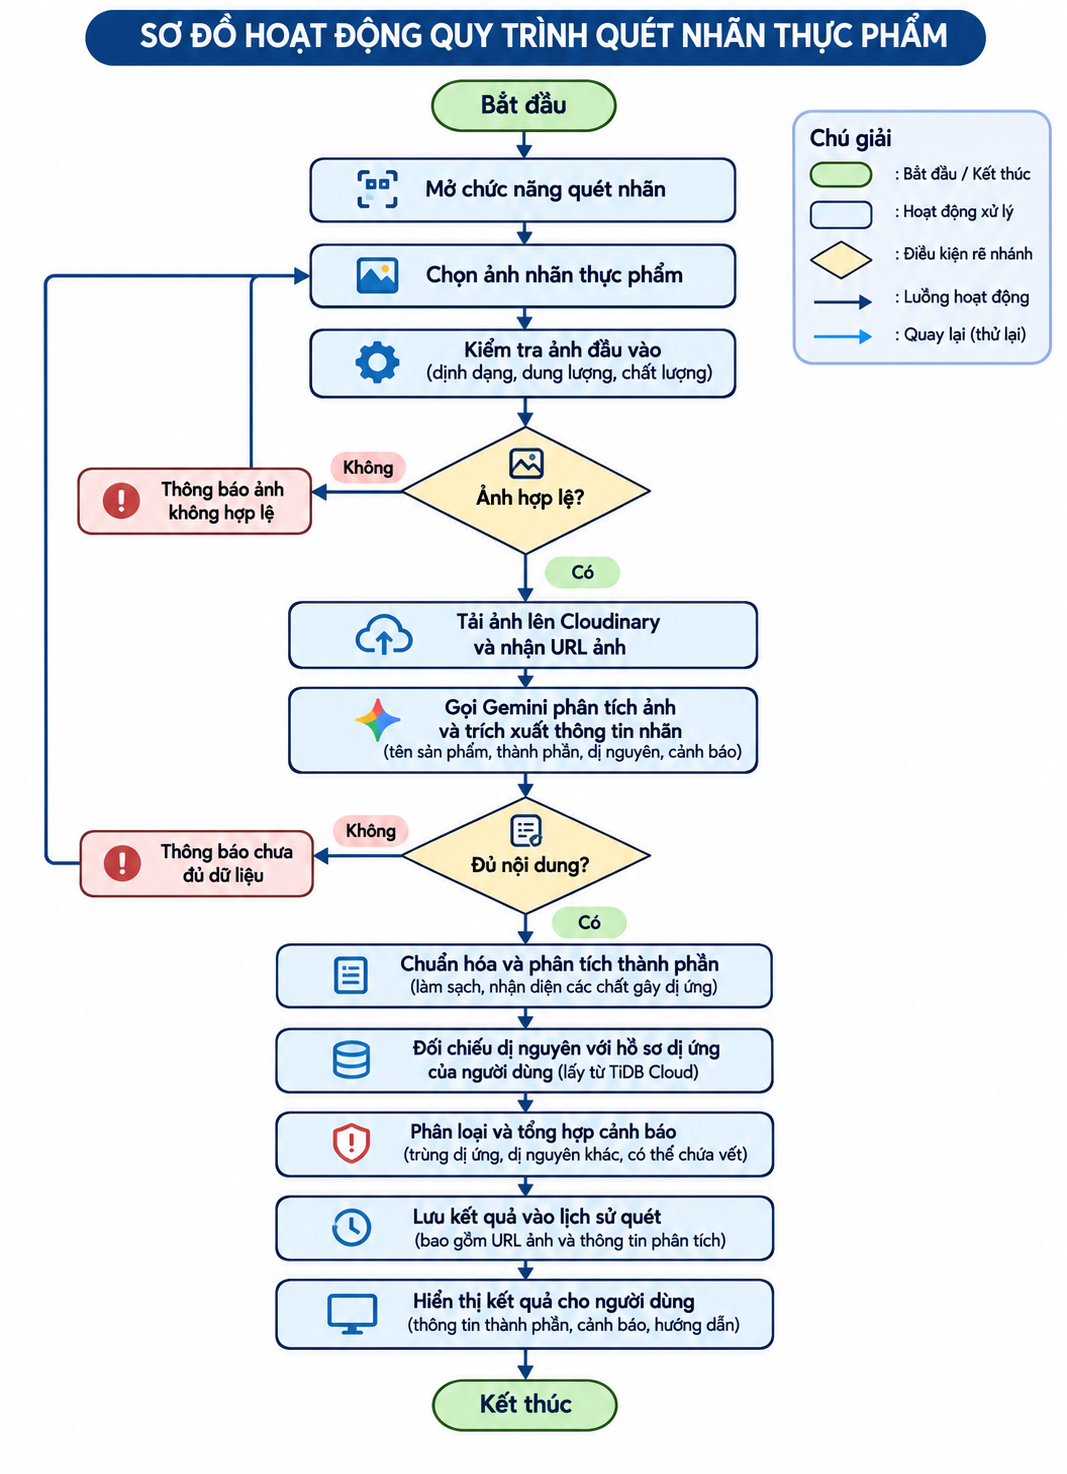
\includegraphics[width=0.72\textwidth,height=0.78\textheight,keepaspectratio]{assets/08_activity_quetnhan.png}
	\caption{Sơ đồ hoạt động quy trình quét nhãn thực phẩm}
	\label{fig:activity-quet-nhan}
\end{figure}

Sơ đồ hoạt động thể hiện luồng xử lý và hai nhánh kiểm tra. Ảnh không hợp lệ hoặc nội dung nhận diện chưa đủ sẽ được thông báo để người dùng thử lại; chỉ khi dữ liệu đạt yêu cầu, hệ thống mới chuẩn hóa, đối chiếu dị nguyên, lưu lịch sử và hiển thị kết quả.


\Needspace{9\baselineskip}
\subsection{Sơ đồ tuần tự quy trình quét nhãn}

Sơ đồ tuần tự mô tả sự trao đổi thông tin giữa người dùng, giao diện web, ứng dụng xử lý nghiệp vụ, thành phần nhận diện và phân tích, cùng cơ sở dữ liệu. Người dùng gửi ảnh từ giao diện; máy chủ tiếp nhận và điều phối quá trình nhận diện, đối chiếu dị nguyên, lưu kết quả rồi trả thông tin phân tích về giao diện.

\begin{figure}[H]
	\centering
	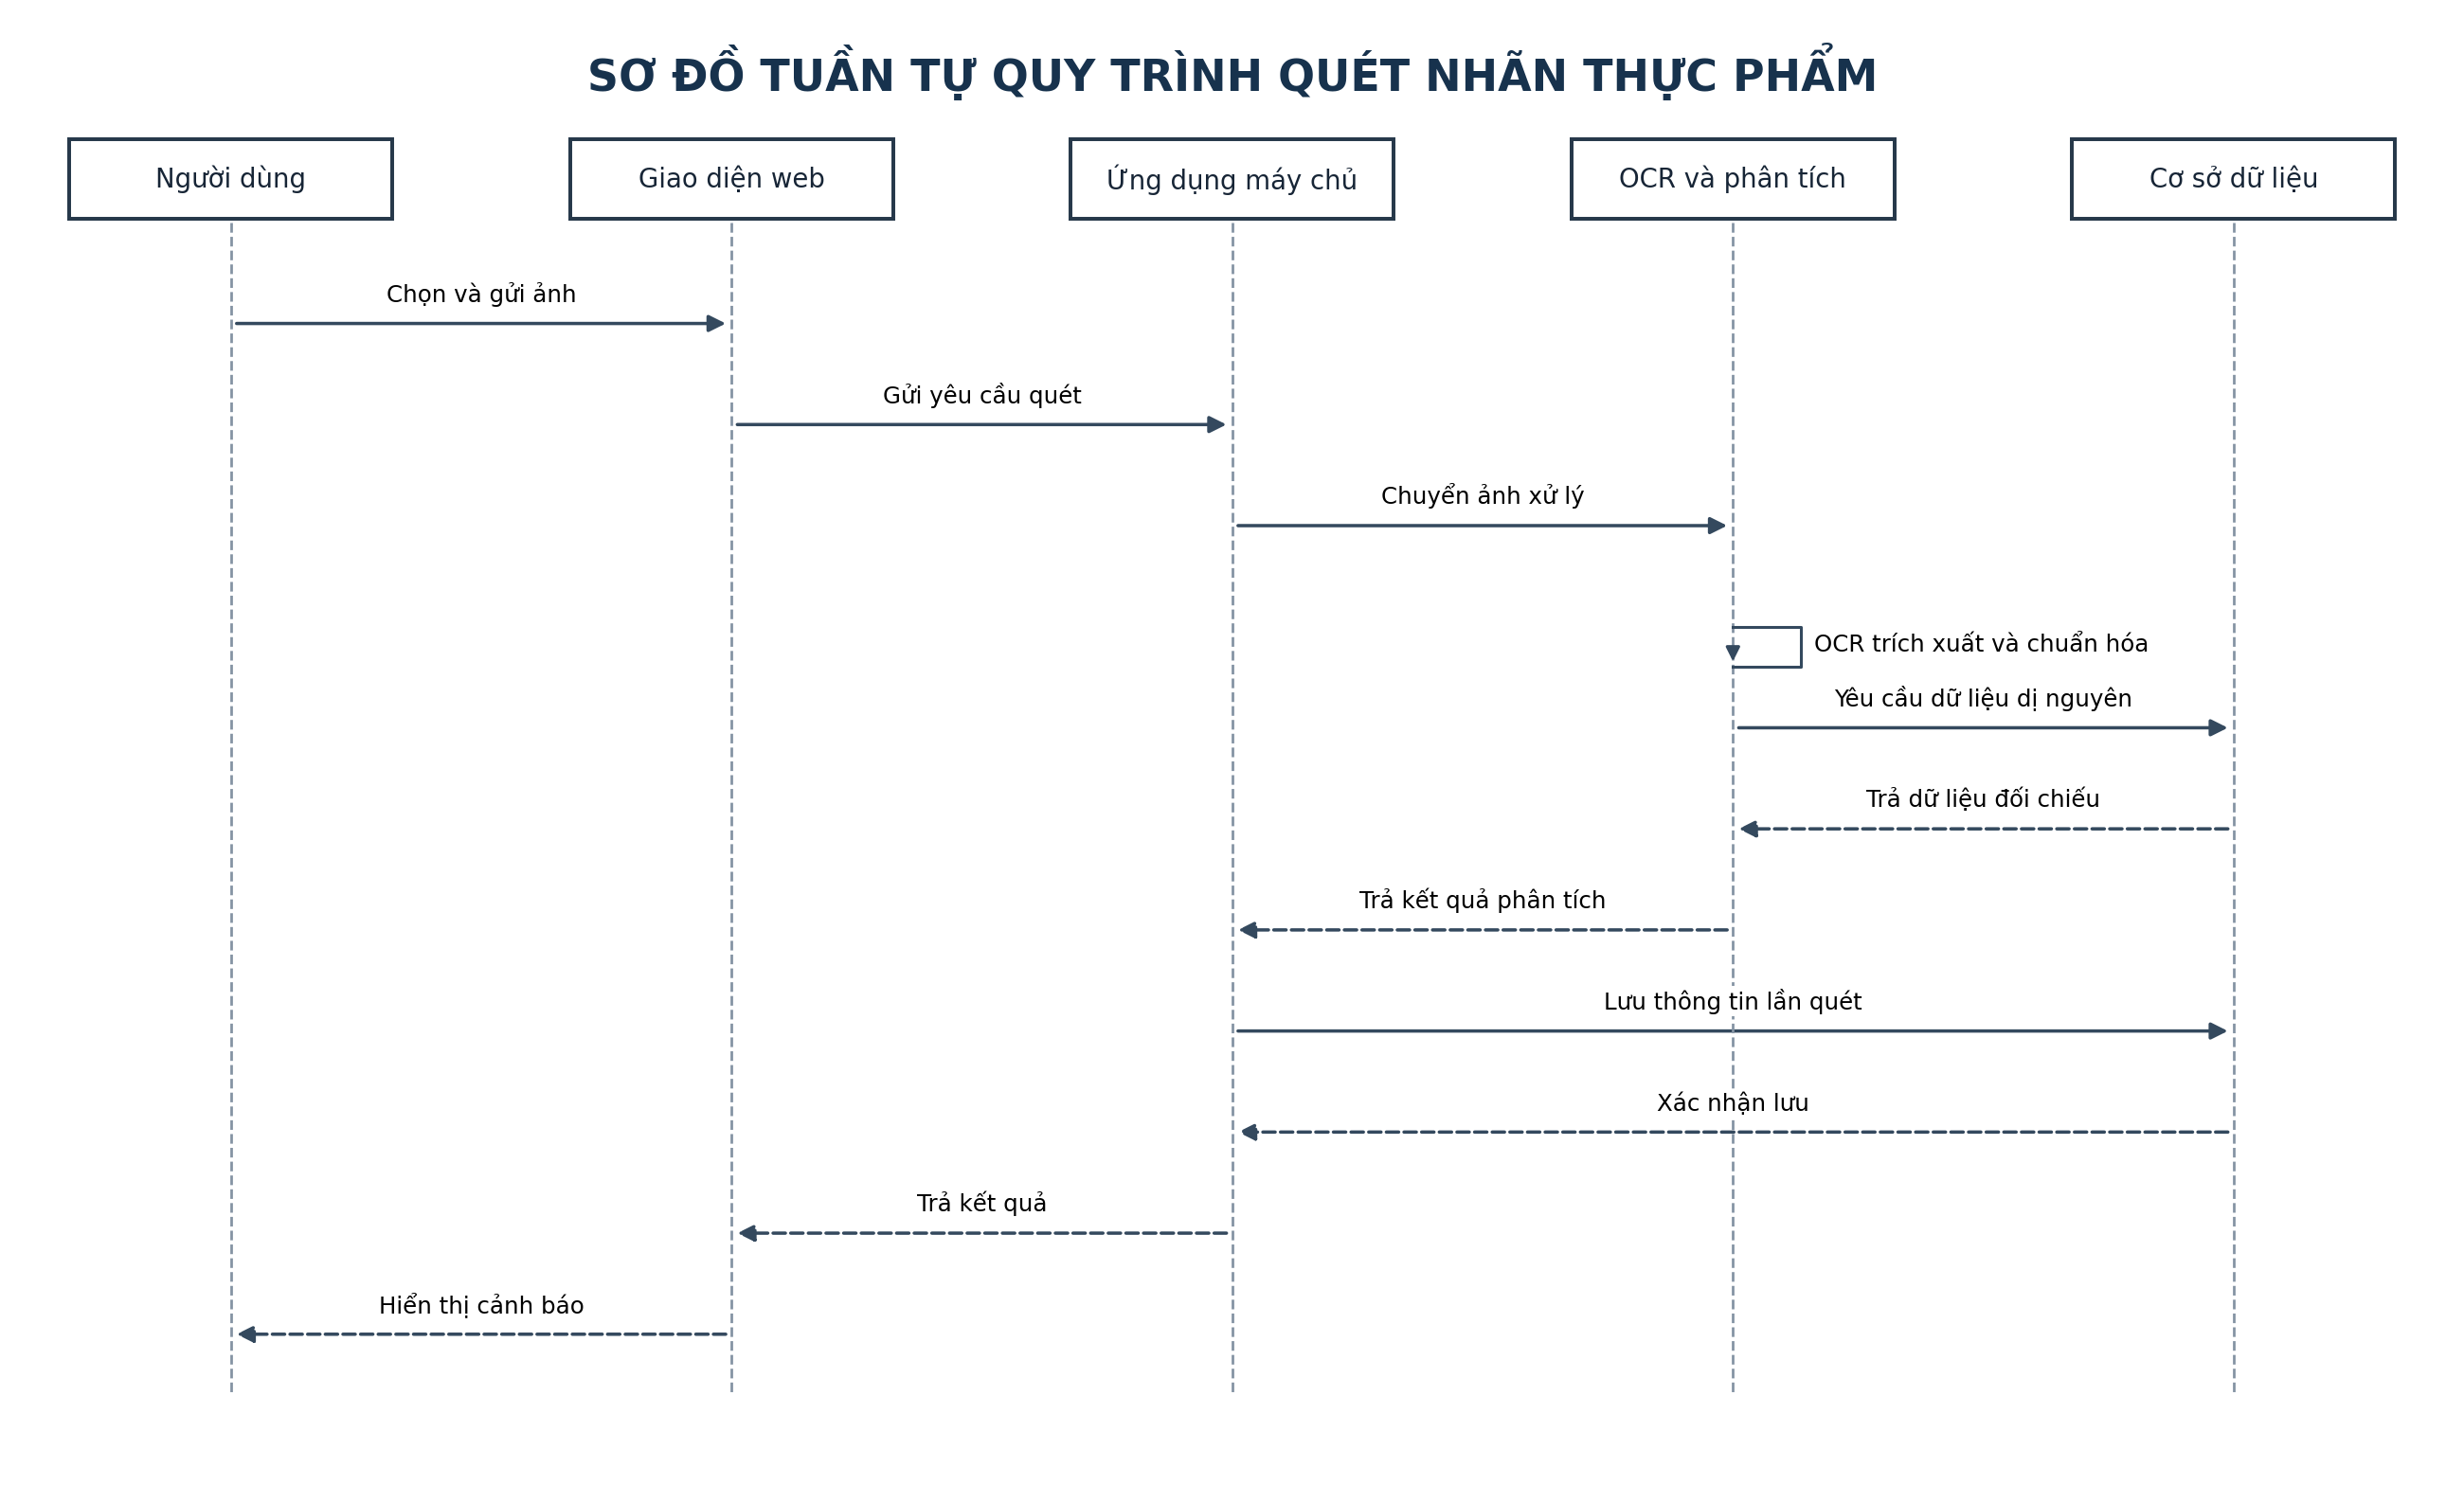
\includegraphics[width=0.95\textwidth,height=0.68\textheight,keepaspectratio]{assets/09_sequence_quetnhan.png}
	\caption{Sơ đồ tuần tự quy trình quét nhãn thực phẩm}
	\label{fig:sequence-quet-nhan}
\end{figure}

Sơ đồ tuần tự mô tả thứ tự trao đổi giữa người dùng, giao diện web, máy chủ, thành phần OCR/phân tích và cơ sở dữ liệu. Máy chủ nhận ảnh, chuyển xử lý, yêu cầu dữ liệu dị nguyên, nhận kết quả, lưu lần quét rồi trả kết quả để giao diện hiển thị cảnh báo.


\Needspace{9\baselineskip}
\subsection{Quy trình phân loại cảnh báo}

Hệ thống cần phân biệt ít nhất hai nhóm thông tin trong kết quả phân tích.

\textbf{Trường hợp thứ nhất: Dị nguyên có bằng chứng trong thành phần.}

Trường hợp này xảy ra khi thông tin thành phần hoặc dữ liệu sản phẩm có nội dung liên quan đến dị nguyên theo quy tắc đối chiếu. Hệ thống hiển thị tên dị nguyên và bằng chứng tương ứng.

\textbf{Trường hợp thứ hai: Cảnh báo có thể chứa vết dị nguyên.}

Trường hợp này được sử dụng khi nhãn có nội dung cảnh báo về khả năng chứa vết dị nguyên nhưng chưa có bằng chứng xác định chắc chắn dị nguyên đó là thành phần thực sự của sản phẩm.

\textbf{Trường hợp thứ ba: Chưa xác định được kết quả.}

Khi dữ liệu đầu vào không đủ hoặc quá trình nhận diện không thu được thông tin cần thiết, hệ thống cần thông báo trạng thái chưa xác định thay vì khẳng định sản phẩm không chứa dị nguyên.

\Needspace{9\baselineskip}
\subsection{Quy trình xem lịch sử quét}

Người dùng truy cập trang lịch sử quét để xem các lần phân tích trước đó. Hệ thống truy xuất những bản ghi liên quan đến tài khoản và hiển thị tên sản phẩm, hình ảnh, thời điểm quét cùng trạng thái cảnh báo.

Việc liên kết lịch sử với tài khoản giúp phân biệt dữ liệu của từng người dùng và hỗ trợ tra cứu lại kết quả đã thực hiện.

% =========================================================
% 3.6 THIẾT KẾ CƠ SỞ DỮ LIỆU
% =========================================================

\Needspace{12\baselineskip}
\section{Thiết kế cơ sở dữ liệu}

\Needspace{9\baselineskip}
\subsection{Mục tiêu thiết kế}

Cơ sở dữ liệu của hệ thống được đặt tên là \texttt{food\_allergen\_system}. Cấu trúc dữ liệu được thiết kế theo mô hình quan hệ, tương thích với MySQL. Trong quá trình phát triển, cơ sở dữ liệu có thể được chạy trên MySQL/MariaDB cục bộ; ở môi trường triển khai trực tuyến, ứng dụng kết nối đến TiDB Cloud. Dữ liệu được chia thành các bảng theo chức năng để quản lý tài khoản, dị nguyên, sản phẩm, thành phần sản phẩm, hồ sơ dị ứng và lịch sử quét.

Việc tách dữ liệu thành các bảng riêng biệt giúp hạn chế lưu trữ trùng lặp, hỗ trợ truy xuất thông tin và xác định mối quan hệ giữa các đối tượng trong hệ thống.

\Needspace{9\baselineskip}
\subsection{Danh sách các bảng dữ liệu}

Cơ sở dữ liệu hiện có sáu bảng chính. Các bảng và trường dưới đây được mô tả theo cấu trúc trong tệp SQL đã cung cấp.

\Needspace{7\baselineskip}
\subsubsection{Bảng allergens}

Bảng \texttt{allergens} lưu danh sách các nhóm dị nguyên được sử dụng trong quá trình đối chiếu.

\begin{table}[H]
	\centering
	\caption{Cấu trúc bảng allergens}
	\label{tab:allergens}
	\small
	\begin{tabularx}{\textwidth}{|l|l|X|l|}
		\hline
		\textbf{Trường} & \textbf{Kiểu dữ liệu} & \textbf{Ý nghĩa} & \textbf{Ràng buộc} \\
		\hline
		id & INT(11) & Mã dị nguyên & Khóa chính, tự tăng \\
		\hline
		name & VARCHAR(100) & Tên dị nguyên bằng tiếng Việt & NOT NULL, UNIQUE \\
		\hline
		description & VARCHAR(255) & Mô tả dị nguyên & Cho phép NULL \\
		\hline
		name\_en & VARCHAR(255) & Tên dị nguyên bằng tiếng Anh & Cho phép NULL \\
		\hline
		off\_tag & VARCHAR(255) & Nhãn dị nguyên theo dữ liệu Open Food Facts & Cho phép NULL \\
		\hline
		created\_at & DATETIME & Thời điểm tạo bản ghi & Mặc định thời gian hiện tại \\
		\hline
	\end{tabularx}
\end{table}

Trường \texttt{id} xác định duy nhất mỗi dị nguyên. Trường \texttt{name} lưu tên hiển thị trên giao diện, còn \texttt{name\_en} và \texttt{off\_tag} hỗ trợ đối chiếu với dữ liệu sản phẩm sử dụng tên tiếng Anh hoặc nhãn chuẩn hóa.

\Needspace{7\baselineskip}
\subsubsection{Bảng products}

Bảng \texttt{products} lưu thông tin sản phẩm thực phẩm đã được thu thập hoặc bổ sung vào hệ thống.

\begin{table}[H]
	\centering
	\caption{Cấu trúc bảng products}
	\label{tab:products}
	\small
	\begin{tabularx}{\textwidth}{|l|l|X|l|}
		\hline
		\textbf{Trường} & \textbf{Kiểu dữ liệu} & \textbf{Ý nghĩa} & \textbf{Ràng buộc} \\
		\hline
		id & INT(11) & Mã sản phẩm & Khóa chính, tự tăng \\
		\hline
		barcode & VARCHAR(50) & Mã vạch sản phẩm & UNIQUE, cho phép NULL \\
		\hline
		name & VARCHAR(255) & Tên sản phẩm & NOT NULL \\
		\hline
		brand & VARCHAR(255) & Thương hiệu sản phẩm & Cho phép NULL \\
		\hline
		ingredients\_text & TEXT & Văn bản thành phần sản phẩm & Cho phép NULL \\
		\hline
		allergens\_text & TEXT & Thông tin dị nguyên được khai báo & Cho phép NULL \\
		\hline
		allergens\_tags & TEXT & Danh sách nhãn dị nguyên & Cho phép NULL \\
		\hline
		image\_url & VARCHAR(1000) & Đường dẫn ảnh sản phẩm & Cho phép NULL \\
		\hline
		source\_url & VARCHAR(1000) & Đường dẫn nguồn dữ liệu & Cho phép NULL \\
		\hline
		created\_at & DATETIME & Thời điểm tạo bản ghi & Mặc định thời gian hiện tại \\
		\hline
	\end{tabularx}
\end{table}

Bảng \texttt{products} lưu các thông tin cơ bản của sản phẩm. Trường \texttt{ingredients\_\allowbreak text} chứa nội dung thành phần dạng văn bản, còn \texttt{allergens\_\allowbreak text} và \texttt{allergens\_\allowbreak tags} lưu thông tin dị nguyên được khai báo. Trường \texttt{image\_\allowbreak url} có thể lưu đường dẫn ảnh sản phẩm và \texttt{source\_\allowbreak url} lưu địa chỉ nguồn dữ liệu khi có.

\Needspace{7\baselineskip}
\subsubsection{Bảng product\_ingredients}

Bảng \texttt{product\_ingredients} lưu từng thành phần của sản phẩm, giúp hệ thống quản lý thành phần dưới dạng các bản ghi riêng.

\begin{table}[H]
	\centering
	\caption{Cấu trúc bảng product\_ingredients}
	\label{tab:product-ingredients}
	\small
	\begin{tabularx}{\textwidth}{|l|l|X|l|}
		\hline
		\textbf{Trường} & \textbf{Kiểu dữ liệu} & \textbf{Ý nghĩa} & \textbf{Ràng buộc} \\
		\hline
		id & INT(11) & Mã thành phần & Khóa chính, tự tăng \\
		\hline
		product\_id & INT(11) & Mã sản phẩm chứa thành phần & Khóa ngoại \\
		\hline
		name & VARCHAR(255) & Tên thành phần & NOT NULL \\
		\hline
		name\_en & VARCHAR(255) & Tên tiếng Anh của thành phần & Cho phép NULL \\
		\hline
		off\_tag & VARCHAR(255) & Nhãn thành phần theo Open Food Facts & Cho phép NULL \\
		\hline
	\end{tabularx}
\end{table}

Trường \texttt{product\_id} liên kết thành phần với bảng \texttt{products}. Khi một sản phẩm có nhiều thành phần, mỗi thành phần được lưu thành một bản ghi riêng. Ràng buộc khóa ngoại được thiết lập để bảo đảm thành phần tham chiếu đến sản phẩm hợp lệ.

\Needspace{7\baselineskip}
\subsubsection{Bảng user}

Bảng \texttt{user} lưu thông tin tài khoản người dùng và trạng thái tài khoản trong hệ thống.

\begin{table}[H]
	\centering
	\caption{Cấu trúc bảng user}
	\label{tab:user}
	\small
	\begin{tabularx}{\textwidth}{|l|l|X|l|}
		\hline
		\textbf{Trường} & \textbf{Kiểu dữ liệu} & \textbf{Ý nghĩa} & \textbf{Ràng buộc} \\
		\hline
		id & CHAR(32) & Mã định danh người dùng & Khóa chính \\
		\hline
		email & VARCHAR(255) & Email đăng nhập & NOT NULL, UNIQUE \\
		\hline
		full\_name & VARCHAR(255) & Họ và tên người dùng & Cho phép NULL \\
		\hline
		hashed\_password & VARCHAR(255) & Giá trị băm của mật khẩu & NOT NULL \\
		\hline
		is\_active & TINYINT(1) & Trạng thái hoạt động của tài khoản & NOT NULL \\
		\hline
		is\_superuser & TINYINT(1) & Xác định tài khoản quản trị & NOT NULL \\
		\hline
		created\_at & DATETIME & Thời điểm tạo tài khoản & Cho phép NULL \\
		\hline
	\end{tabularx}
\end{table}

Trường \texttt{id} dùng để định danh tài khoản. Trường \texttt{email} có ràng buộc duy nhất nhằm hạn chế tạo nhiều tài khoản cùng email. Trường \texttt{hashed\_password} lưu giá trị băm mật khẩu, không lưu mật khẩu ở dạng văn bản thông thường. Hai trường \texttt{is\_active} và \texttt{is\_superuser} thể hiện trạng thái hoạt động và quyền quản trị của tài khoản.

\Needspace{7\baselineskip}
\subsubsection{Bảng user\_allergens}

Bảng \texttt{user\_allergens} liên kết người dùng với các nhóm dị nguyên mà họ lựa chọn trong hồ sơ cá nhân.

\begin{table}[H]
	\centering
	\caption{Cấu trúc bảng user\_allergens}
	\label{tab:user-allergens}
	\small
	\begin{tabularx}{\textwidth}{|l|l|X|l|}
		\hline
		\textbf{Trường} & \textbf{Kiểu dữ liệu} & \textbf{Ý nghĩa} & \textbf{Ràng buộc} \\
		\hline
		id & INT(11) & Mã bản ghi hồ sơ dị ứng & Khóa chính, tự tăng \\
		\hline
		user\_id & CHAR(32) & Mã người dùng & Khóa ngoại \\
		\hline
		allergen\_id & INT(11) & Mã dị nguyên được lựa chọn & Khóa ngoại \\
		\hline
		created\_at & DATETIME & Thời điểm thêm dị nguyên & Mặc định thời gian hiện tại \\
		\hline
	\end{tabularx}
\end{table}

Trường \texttt{user\_id} liên kết với bảng \texttt{user}, còn \texttt{allergen\_id} liên kết với bảng \texttt{allergens}. Cặp trường \texttt{user\_id} và \texttt{allergen\_id} có ràng buộc duy nhất kết hợp, nhằm tránh lưu trùng cùng một dị nguyên cho một người dùng.

\Needspace{7\baselineskip}
\subsubsection{Bảng scan\_history}

Bảng \texttt{scan\_history} lưu lịch sử phân tích nhãn thực phẩm của người dùng.

\begin{table}[H]
	\centering
	\caption{Cấu trúc bảng scan\_history}
	\label{tab:scan-history}
	\scriptsize
	\begin{tabularx}{\textwidth}{|l|l|X|l|}
		\hline
		\textbf{Trường} & \textbf{Kiểu dữ liệu} & \textbf{Ý nghĩa} & \textbf{Ràng buộc} \\
		\hline
		id & INT(11) & Mã bản ghi lịch sử & Khóa chính, tự tăng \\
		\hline
		scan\_id & VARCHAR(32) & Mã định danh lần quét & NOT NULL, UNIQUE \\
		\hline
		user\_id & CHAR(32) & Người thực hiện quét & Khóa ngoại, NOT NULL \\
		\hline
		product\_id & INT(11) & Mã sản phẩm liên quan nếu xác định được & Khóa ngoại, cho phép NULL \\
		\hline
		product\_name & VARCHAR(255) & Tên sản phẩm được nhận diện & NOT NULL \\
		\hline
		brand & VARCHAR(255) & Thương hiệu sản phẩm & Cho phép NULL \\
		\hline
		image\_url & VARCHAR(1000) & Đường dẫn ảnh đã tải lên & Cho phép NULL \\
		\hline
		ingredients\_json & TEXT & Danh sách thành phần ở dạng JSON & NOT NULL \\
		\hline
		allergens\_json & TEXT & Danh sách dị nguyên ở dạng JSON & NOT NULL \\
		\hline
		warnings\_json & TEXT & Chi tiết cảnh báo ở dạng JSON & NOT NULL \\
		\hline
		warning\_status & VARCHAR(20) & Trạng thái cảnh báo & NOT NULL \\
		\hline
		scanned\_at & DATETIME & Thời điểm thực hiện quét & NOT NULL, mặc định thời gian hiện tại \\
		\hline
	\end{tabularx}
\end{table}

Bảng \texttt{scan\_history} lưu kết quả của từng lần quét. Các trường \texttt{ingredients\_json}, \texttt{allergens\_json} và \texttt{warnings\_json} lưu dữ liệu có cấu trúc JSON dưới dạng văn bản. Cách tổ chức này cho phép lưu danh sách thành phần, dị nguyên và chi tiết cảnh báo của từng lần phân tích.

Trường \texttt{warning\_status} thể hiện trạng thái kết quả, còn \texttt{scanned\_at} lưu thời điểm thực hiện. Trường \texttt{product\_id} có thể để trống khi hệ thống chưa xác định được sản phẩm tương ứng.

\Needspace{9\baselineskip}
\subsection{Mối quan hệ giữa các bảng}

Cơ sở dữ liệu sử dụng các khóa chính và khóa ngoại để liên kết sáu bảng. Các quan hệ chính gồm:

\begin{itemize}
	\item \texttt{user} -- \texttt{scan\_history}: quan hệ một-nhiều. Một người dùng có thể thực hiện nhiều lần quét; mỗi bản ghi lịch sử thuộc về một người dùng thông qua \texttt{user\_id}.
	\item \texttt{products} -- \texttt{scan\_history}: quan hệ một-nhiều. Một sản phẩm có thể xuất hiện trong nhiều lần quét. Trường \texttt{product\_id} trong lịch sử cho phép NULL nếu chưa xác định được sản phẩm.
	\item \texttt{products} -- \texttt{product\_ingredients}: quan hệ một-nhiều. Một sản phẩm có thể có nhiều thành phần; mỗi thành phần tham chiếu sản phẩm qua \texttt{product\_id}.
	\item \texttt{user} -- \texttt{user\_allergens}: quan hệ một-nhiều. Một người dùng có thể lưu nhiều dị nguyên quan tâm.
	\item \texttt{allergens} -- \texttt{user\_allergens}: quan hệ một-nhiều. Một dị nguyên có thể được nhiều người dùng lựa chọn.
\end{itemize}

Do đó, \texttt{user} và \texttt{allergens} có quan hệ nhiều-nhiều thông qua bảng trung gian \texttt{user\_allergens}. Bảng này có ràng buộc UNIQUE kết hợp trên \texttt{(user\_id, allergen\_id)} để tránh một người dùng lưu trùng cùng dị nguyên.

\Needspace{9\baselineskip}
\subsection{Sơ đồ ERD tổng quát}

Sơ đồ ERD cập nhật thể hiện sáu bảng đang được sử dụng trong cơ sở dữ liệu Allergy Warning: \texttt{user}, \texttt{scan\_history}, \texttt{products}, \texttt{user\_allergens}, \texttt{allergens} và \texttt{product\_ingredients}. Sơ đồ thể hiện rõ khóa chính (PK), khóa ngoại (FK), khóa duy nhất (UQ), kiểu dữ liệu và lực lượng quan hệ giữa các bảng.

Trong phiên bản này, bảng \texttt{scan\_history} có thêm các trường \texttt{may\_contain\_json}, \texttt{comparison\_status}, \texttt{previous\_warnings\_json} và \texttt{previous\_comparison\_status}. Các trường này lưu thông tin cảnh báo có thể chứa vết và trạng thái so sánh/cảnh báo trước đó của lần quét. Bảng \texttt{product\_ingredients} cũng được bổ sung các trường chuẩn hóa gồm \texttt{normalized\_name}, \texttt{normalized\_name\_en}, \texttt{standard\_key} và \texttt{normalization\_status} để hỗ trợ chuẩn hóa tên thành phần.

Quan hệ trong sơ đồ được hiểu như sau: một người dùng có nhiều bản ghi lịch sử quét và nhiều lựa chọn dị nguyên; một sản phẩm có thể xuất hiện trong nhiều bản ghi quét và có nhiều thành phần; một dị nguyên có thể được nhiều người dùng lựa chọn. Trường \texttt{product\_id} trong \texttt{scan\_history} là khóa ngoại có thể NULL, vì vậy hệ thống vẫn lưu được lịch sử khi chưa ghép được lần quét với sản phẩm trong danh mục.

\begin{figure}[H]
	\centering
	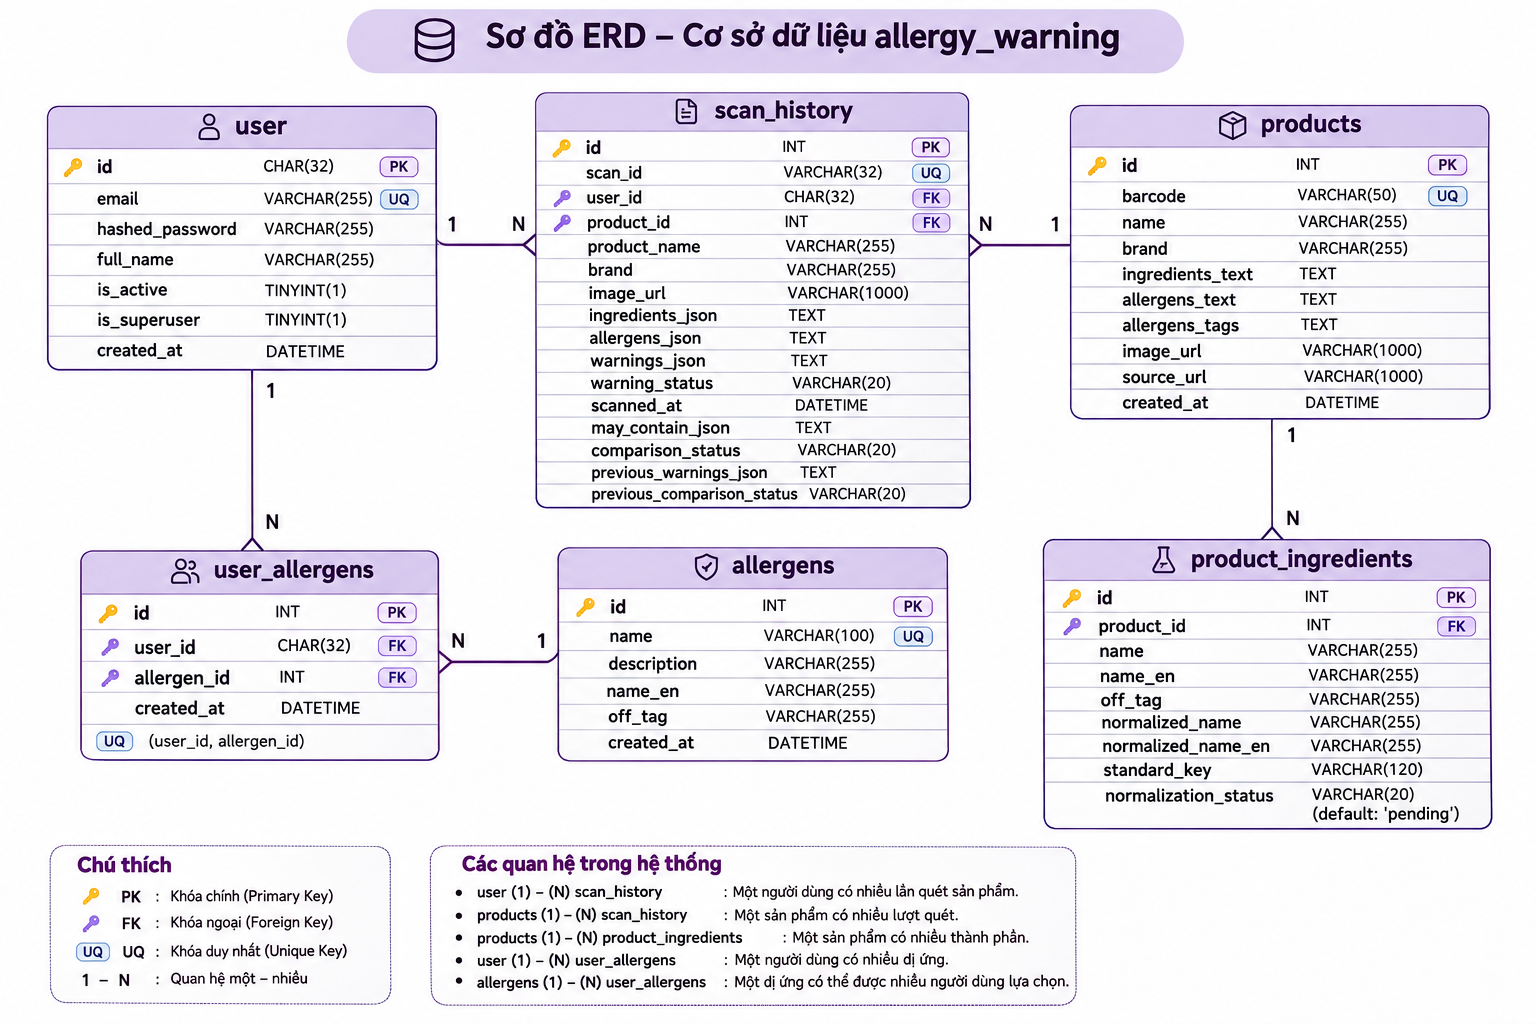
\includegraphics[width=0.98\textwidth,height=0.72\textheight,keepaspectratio]{assets/10_erd_co_so_du_lieu.png}
	\caption{Sơ đồ ERD cập nhật của cơ sở dữ liệu Allergy Warning}
	\label{fig:erd-allergy-warning}
\end{figure}

Sơ đồ cho thấy \texttt{scan\_history} liên kết trực tiếp với \texttt{user} và \texttt{products}; không có quan hệ trực tiếp giữa \texttt{scan\_history} và \texttt{product\_ingredients}. Bảng \texttt{product\_ingredients} chỉ liên kết với \texttt{products} thông qua \texttt{product\_id}. Đây là điểm cần lưu ý để bảo đảm phần mô tả và sơ đồ thống nhất với cấu trúc khóa ngoại thực tế.

\Needspace{9\baselineskip}
\subsection{Nguyên tắc bảo đảm dữ liệu}

\textbf{Tính toàn vẹn:}

Các bảng sử dụng khóa chính để xác định bản ghi. Những mối quan hệ cần thiết được thiết lập bằng khóa ngoại, giúp dữ liệu liên kết đúng đối tượng.

\textbf{Tính duy nhất:}

Email người dùng, tên dị nguyên, mã vạch sản phẩm và mã lần quét có các ràng buộc duy nhất theo cấu trúc cơ sở dữ liệu. Bảng \texttt{user\_allergens} cũng có ràng buộc duy nhất kết hợp giữa người dùng và dị nguyên.

\textbf{Tính nhất quán:}

Thông tin dị nguyên được lưu tập trung trong bảng \texttt{allergens}. Hồ sơ dị ứng tham chiếu đến bảng này, giúp hạn chế việc mỗi người dùng lưu một cách biểu diễn riêng cho cùng một dị nguyên.

\textbf{Tính bảo mật:}

Mật khẩu được lưu dưới dạng giá trị băm trong trường \texttt{hashed\_password}. Việc truy cập lịch sử quét và hồ sơ cá nhân cần được giới hạn theo tài khoản tương ứng.

\textbf{Khả năng mở rộng:}

Cấu trúc bảng cho phép bổ sung sản phẩm, thành phần và nhóm dị nguyên mới. Lịch sử quét cũng có thể lưu nhiều lần phân tích của một người dùng.

% =========================================================
% 3.7 THIẾT KẾ GIAO DIỆN
% =========================================================

\Needspace{12\baselineskip}
\section{Thiết kế giao diện hệ thống}

\Needspace{9\baselineskip}
\subsection{Giao diện đăng nhập}

Giao diện đăng nhập cho phép người dùng nhập email và mật khẩu để truy cập hệ thống. Trang được chia thành khu vực giới thiệu hệ thống và khu vực nhập thông tin tài khoản. Cách bố trí này giúp người dùng dễ nhận biết mục đích của ứng dụng và thao tác đăng nhập.

\begin{figure}[H]
	\centering
	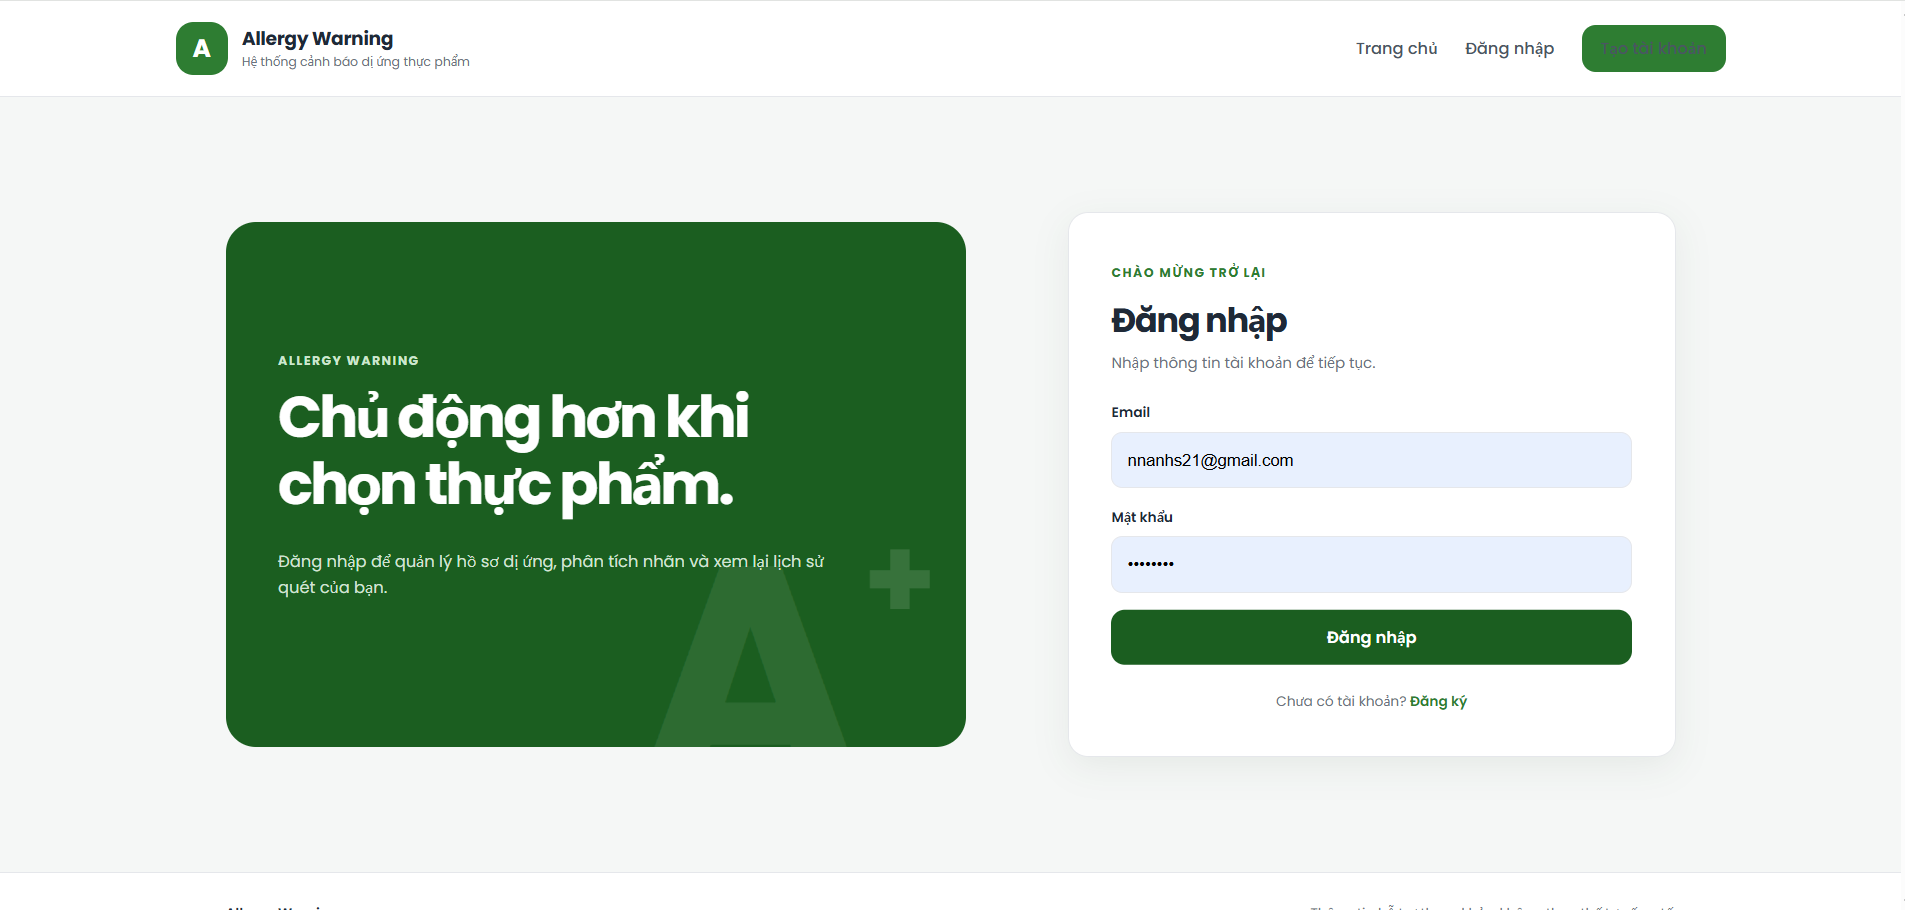
\includegraphics[width=0.90\textwidth,height=0.62\textheight,keepaspectratio]{assets/Login.png}
	\caption{Giao diện đăng nhập hệ thống Allergy Warning}
	\label{fig:giao-dien-dang-nhap}
\end{figure}

Hình minh họa trang đăng nhập, nơi người dùng nhập email và mật khẩu để xác thực trước khi truy cập các chức năng cần tài khoản.


\Needspace{9\baselineskip}
\subsection{Giao diện đăng ký tài khoản}

Giao diện đăng ký cung cấp các trường nhập họ tên, email, mật khẩu và xác nhận mật khẩu. Người dùng nhập thông tin theo yêu cầu của biểu mẫu để tạo tài khoản mới.

\begin{figure}[H]
	\centering
	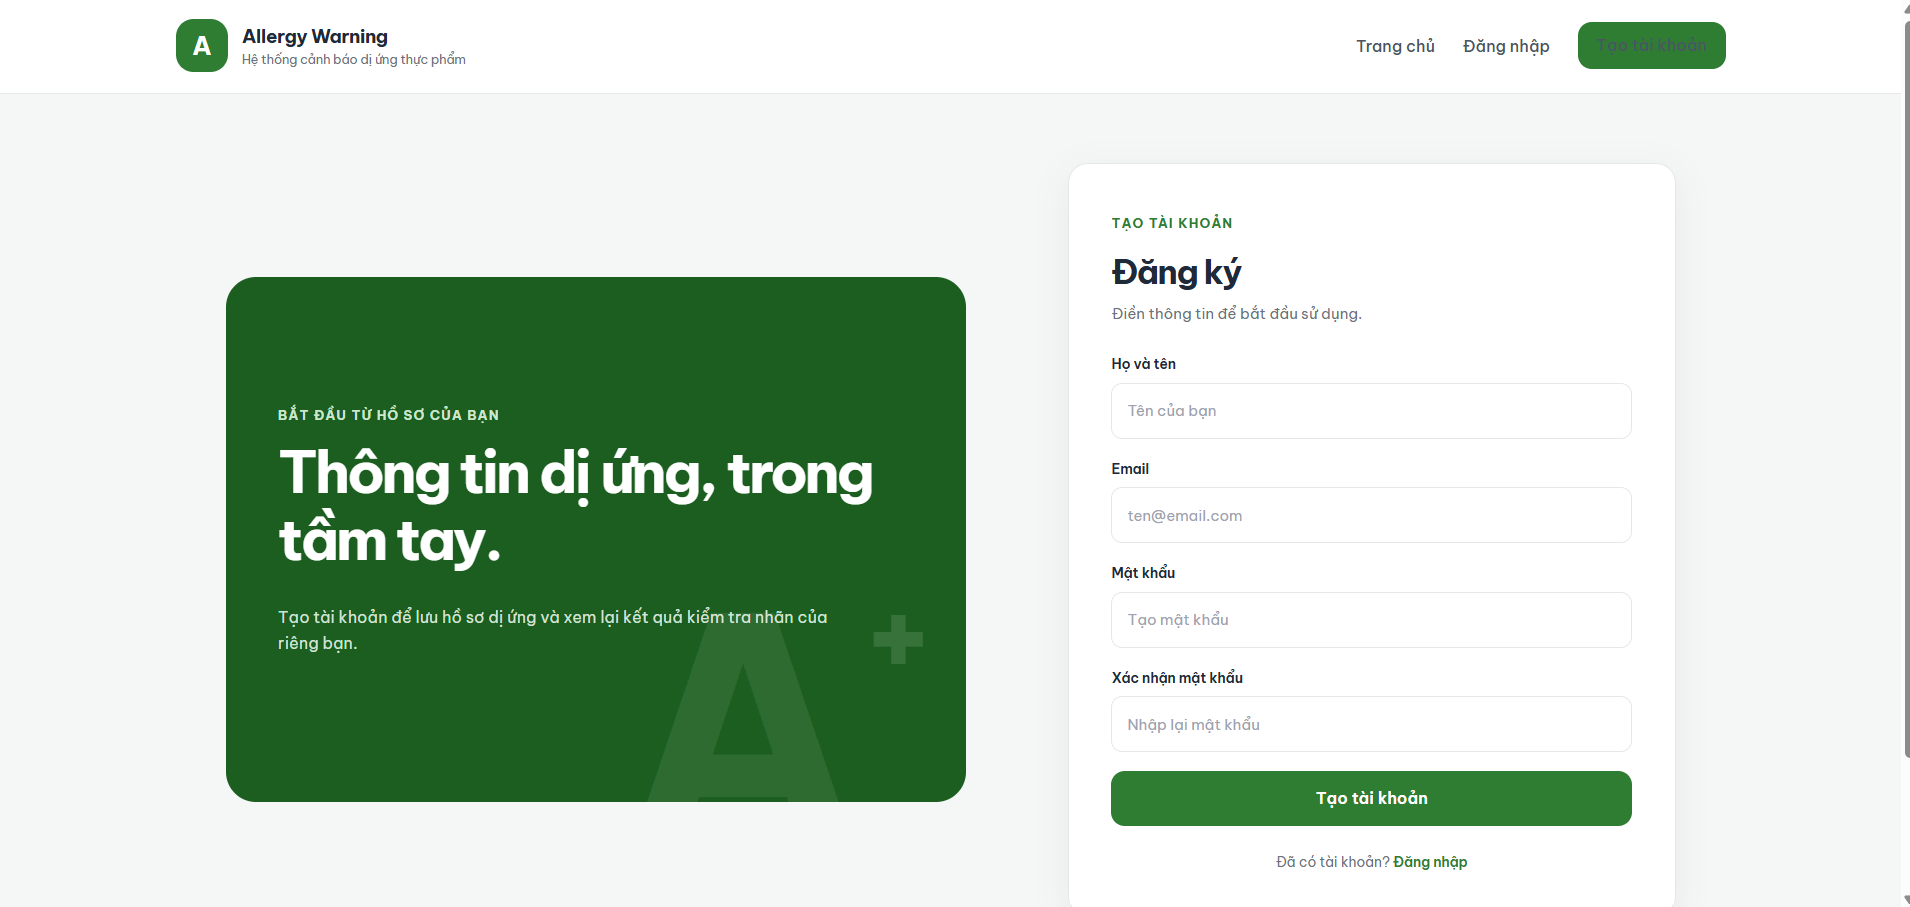
\includegraphics[width=0.90\textwidth,height=0.62\textheight,keepaspectratio]{assets/register.png}
	\caption{Giao diện đăng ký tài khoản}
	\label{fig:giao-dien-dang-ky}
\end{figure}

Hình minh họa biểu mẫu đăng ký, cho phép người dùng nhập thông tin cần thiết để tạo tài khoản mới.


\Needspace{9\baselineskip}
\subsection{Giao diện Dashboard người dùng}

Dashboard là trang tổng quan sau khi người dùng đăng nhập. Giao diện hiển thị lời chào, các lối truy cập nhanh đến chức năng quét nhãn, hồ sơ dị ứng và lịch sử quét. Khu vực hoạt động gần đây giúp người dùng theo dõi các sản phẩm đã phân tích.

\begin{figure}[H]
	\centering
	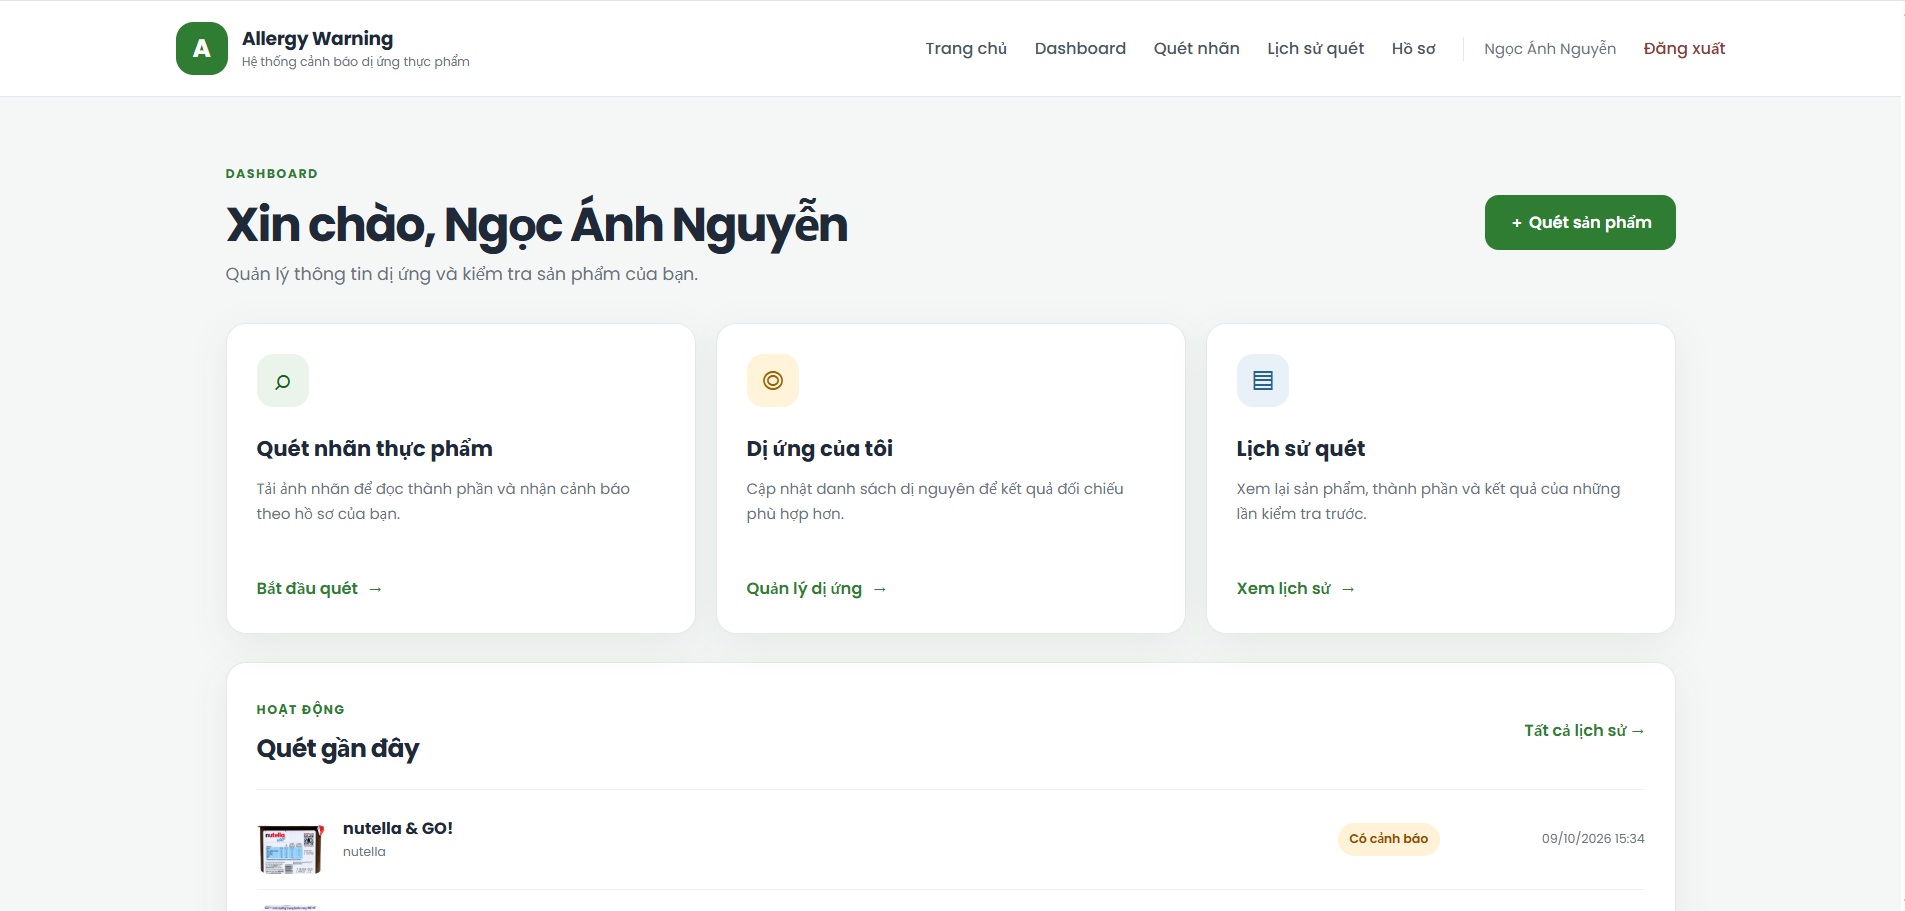
\includegraphics[width=0.95\textwidth,height=0.62\textheight,keepaspectratio]{assets/Dashboard.png}
	\caption{Giao diện Dashboard dành cho người dùng}
	\label{fig:giao-dien-dashboard}
\end{figure}

Hình minh họa trang tổng quan sau đăng nhập, cung cấp lối truy cập đến các chức năng chính và thông tin hoạt động của người dùng.


\Needspace{9\baselineskip}
\subsection{Giao diện hồ sơ cá nhân}

Giao diện hồ sơ cá nhân cung cấp thông tin tài khoản và những thông tin chất gây dị ứng  liên quan đến người dùng.

\begin{figure}[H]
	\centering
	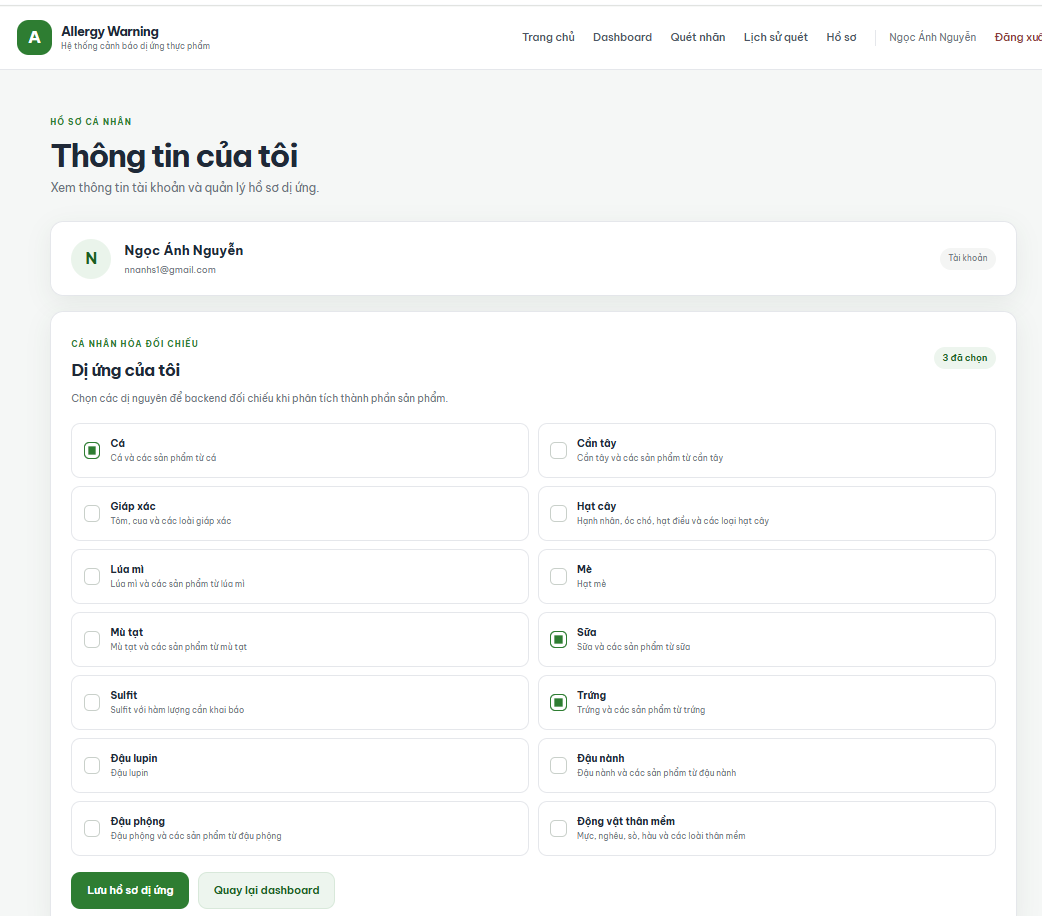
\includegraphics[width=0.90\textwidth,height=0.62\textheight,keepaspectratio]{assets/profile.png}
	\caption{Giao diện hồ sơ cá nhân - phần thông tin dị ứng của  tài khoản}
	\label{fig:giao-dien-ho-so-1}
\end{figure}

Hình thể hiện khu vực thông tin tài khoản trong trang hồ sơ cá nhân, giúp người dùng có thể kiểm tra, theo dõi hoặc cập nhật lại thông tin của bản thân.

\Needspace{9\baselineskip}
\subsection{Giao diện quét nhãn thực phẩm}

Giao diện quét nhãn cho phép người dùng tải ảnh từ thiết bị. Sau khi chọn ảnh, hệ thống hiển thị ảnh hoặc tên tệp và nút bắt đầu phân tích. Phần hướng dẫn trên giao diện cung cấp thông tin về định dạng ảnh được hỗ trợ.

\begin{figure}[H]
	\centering
	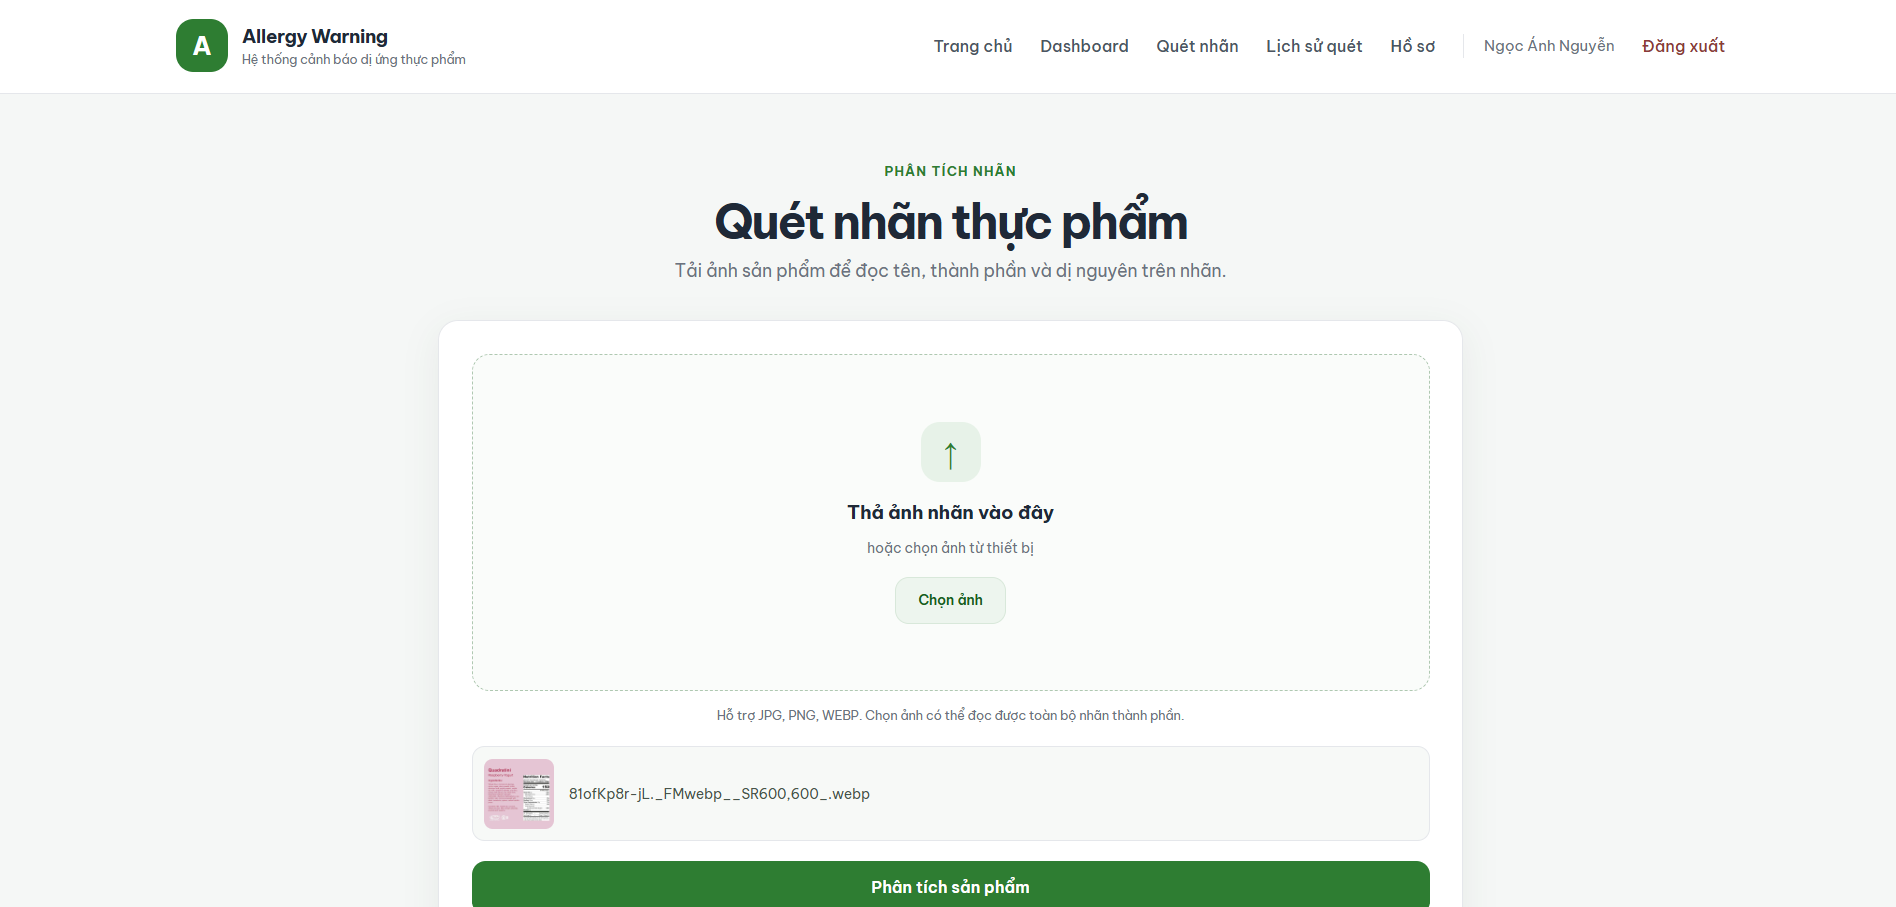
\includegraphics[width=0.90\textwidth,height=0.62\textheight,keepaspectratio]{assets/scan.png}
	\caption{Giao diện tải ảnh nhãn thực phẩm}
	\label{fig:giao-dien-quet-nhan}
\end{figure}

Hình minh họa giao diện chọn và tải ảnh nhãn thực phẩm trước khi gửi yêu cầu phân tích.


\Needspace{9\baselineskip}
\subsection{Giao diện lịch sử quét}

Giao diện lịch sử quét giúp người dùng xem lại các sản phẩm đã được phân tích. Mỗi bản ghi có thể hiển thị tên sản phẩm, hình ảnh, trạng thái cảnh báo và thời gian thực hiện.

\begin{figure}[H]
	\centering
	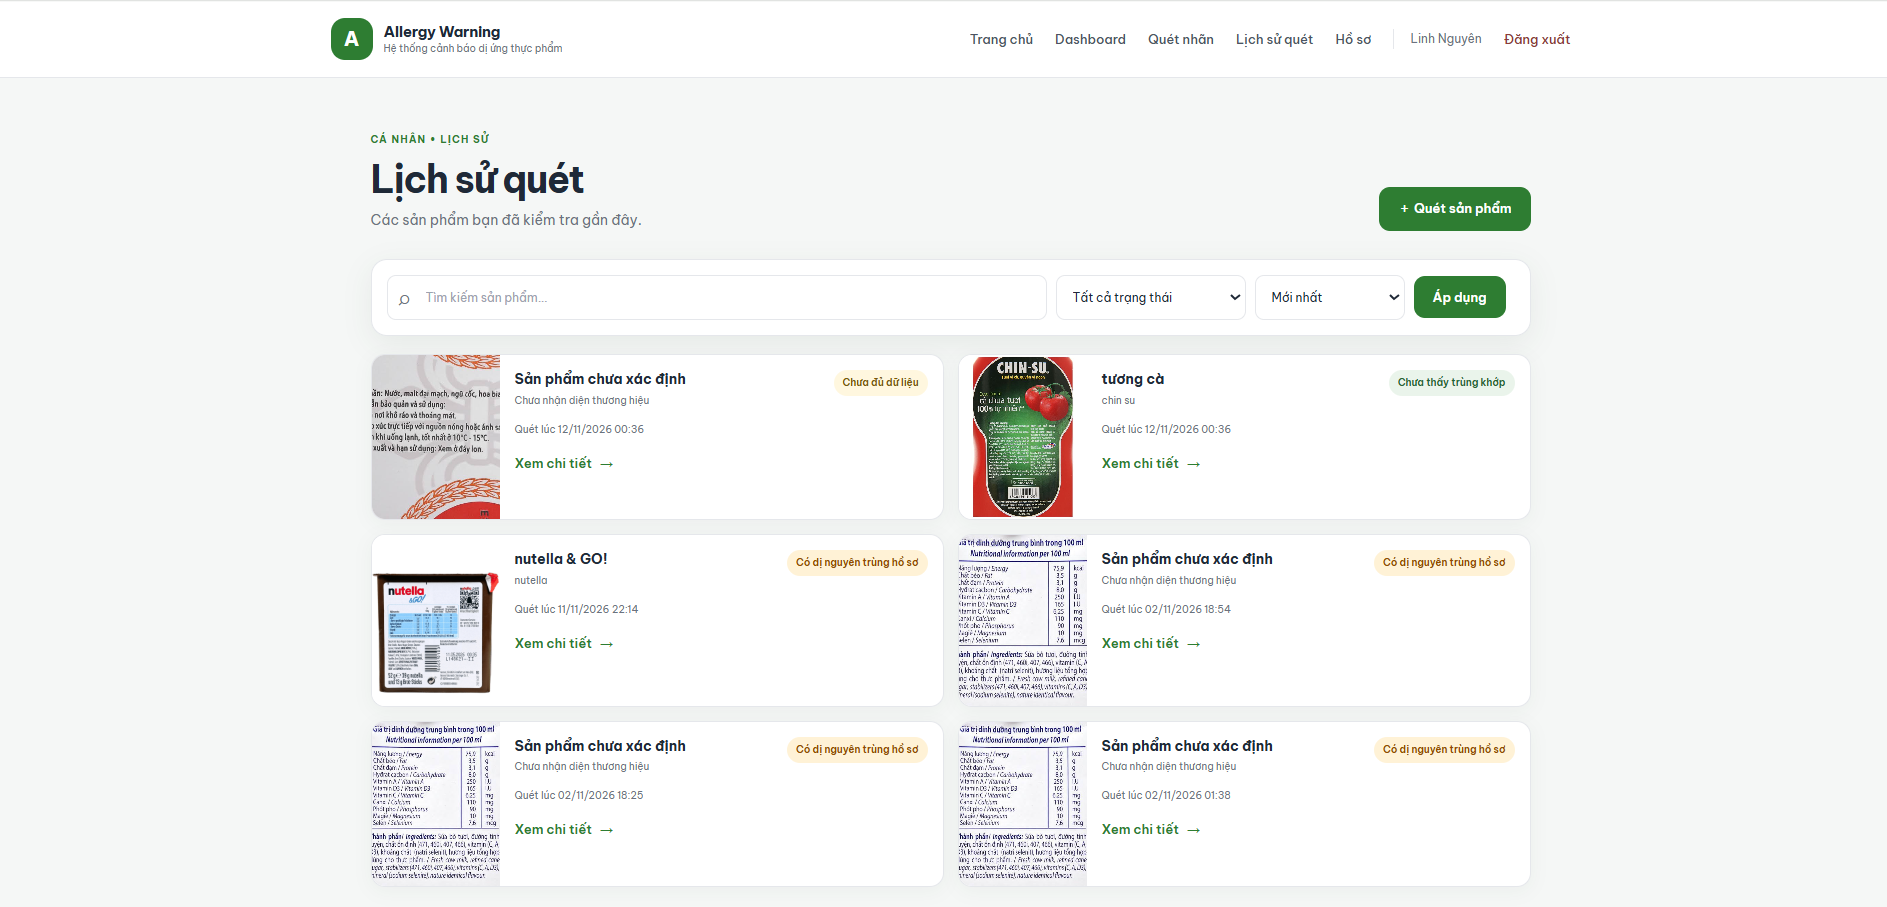
\includegraphics[width=0.95\textwidth,height=0.62\textheight,keepaspectratio]{assets/scan_history.png}
	\caption{Giao diện danh sách lịch sử quét}
	\label{fig:giao-dien-lich-su}
\end{figure}

Hình minh họa danh sách các lần quét đã lưu, giúp người dùng tra cứu sản phẩm, thời điểm và trạng thái cảnh báo.


\Needspace{9\baselineskip}
\subsection{Giao diện chi tiết lịch sử quét}

Các ảnh chi tiết lịch sử quét minh họa những phần thông tin khác nhau của một bản ghi, bao gồm thông tin sản phẩm, nội dung phân tích và cảnh báo dị nguyên. Việc tách thành nhiều ảnh giúp thể hiện đầy đủ nội dung của trang chi tiết.

\begin{figure}[H]
	\centering
	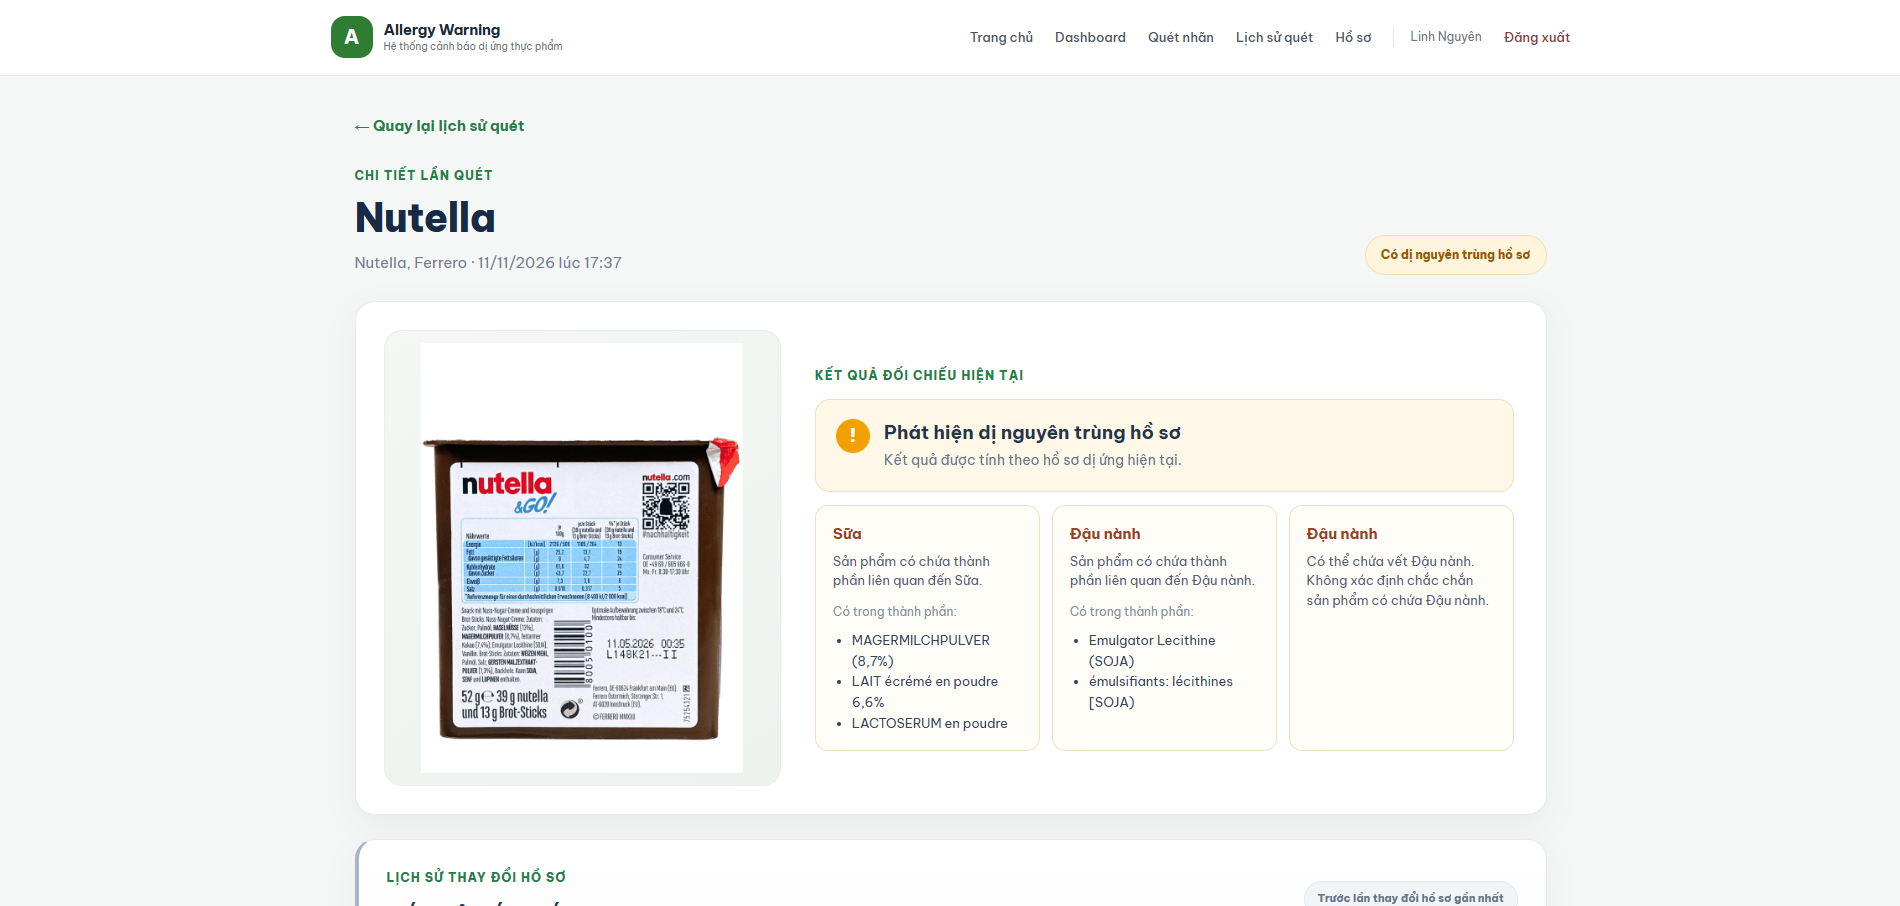
\includegraphics[width=0.90\textwidth,height=0.62\textheight,keepaspectratio]{assets/scan_history_product_detail1.png}
	\caption{Chi tiết lịch sử quét - thông tin sản phẩm}
	\label{fig:lich-su-chi-tiet-1}
\end{figure}

Hình thể hiện phần thông tin sản phẩm của một bản ghi lịch sử quét, giúp người dùng nhận biết sản phẩm đã được phân tích.


\begin{figure}[H]
	\centering
	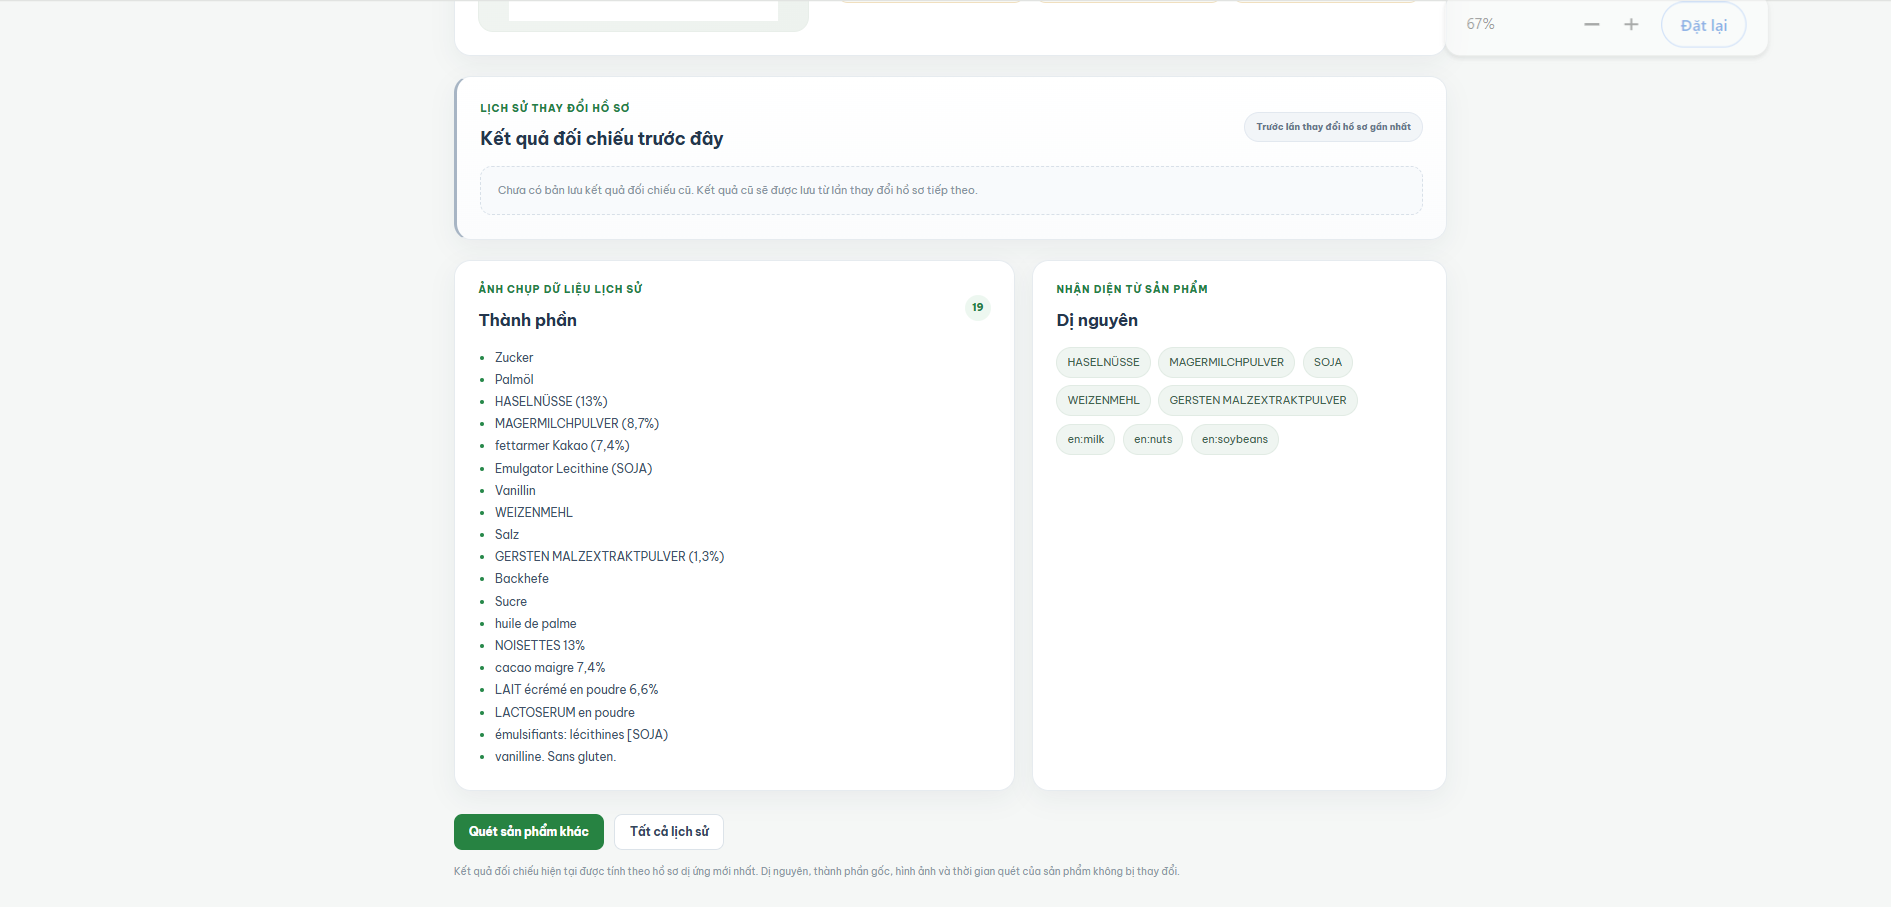
\includegraphics[width=0.90\textwidth,height=0.62\textheight,keepaspectratio]{assets/scan_history_product_detail2.png}
	\caption{Chi tiết lịch sử quét - thông tin phân tích}
	\label{fig:lich-su-chi-tiet-2}
\end{figure}

Hình thể hiện phần thông tin phân tích của bản ghi, bổ sung chi tiết thành phần và kết quả cảnh báo tương ứng.




\Needspace{9\baselineskip}
\subsection{Giao diện kết quả phân tích}

Giao diện kết quả phân tích hiển thị thông tin thu được sau khi hệ thống xử lý ảnh nhãn thực phẩm. Ba hình ảnh liên tiếp minh họa ba phần của cùng một trang kết quả, không phải ba giao diện độc lập.

Phần đầu giao diện hiển thị tên sản phẩm, thương hiệu, hình ảnh nhãn thực phẩm và trạng thái cảnh báo tổng quan. Phần tiếp theo trình bày danh sách thành phần được nhận diện và các dị nguyên được phát hiện. Phần cuối trình bày chi tiết cảnh báo dị nguyên, bao gồm các dị nguyên có bằng chứng trong danh sách thành phần và những thông tin cảnh báo có thể chứa vết dị nguyên trên nhãn.

\begin{figure}[H]
	\centering
	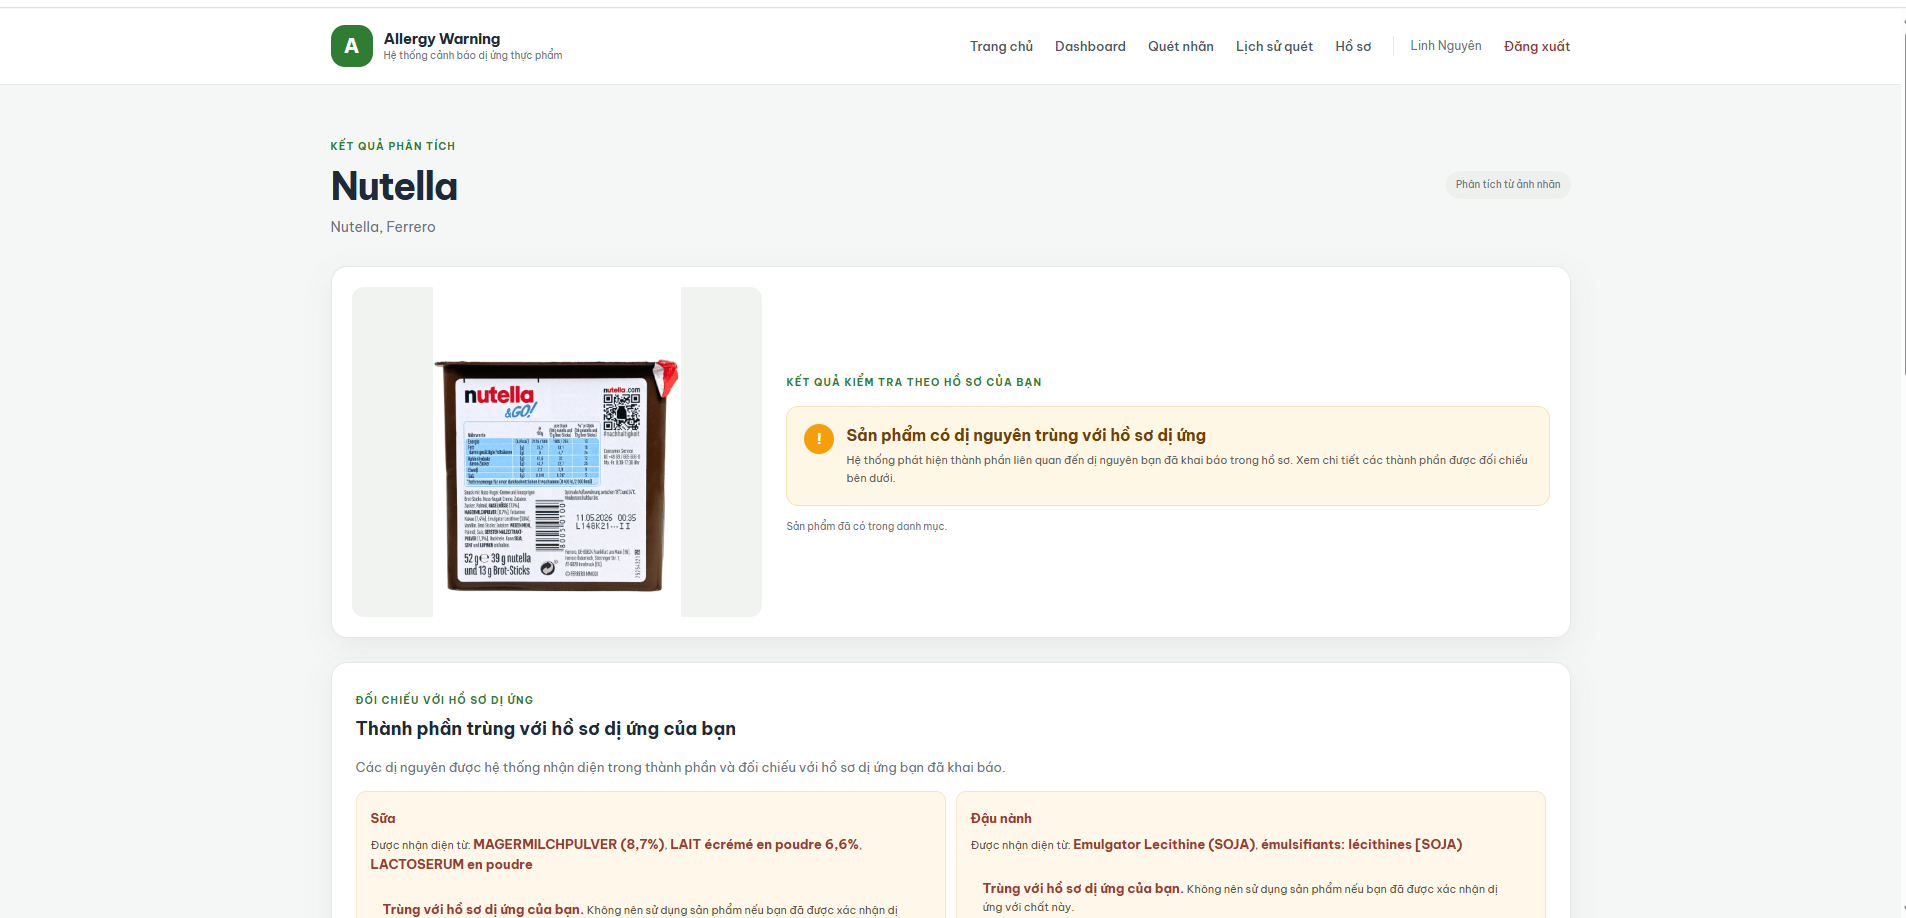
\includegraphics[width=0.90\textwidth,height=0.62\textheight,keepaspectratio]{assets/result1.png}
	\caption{Phần đầu giao diện kết quả phân tích sản phẩm}
	\label{fig:giao-dien-ket-qua-1}
\end{figure}

Hình minh họa phần đầu trang kết quả, gồm thông tin nhận diện sản phẩm và trạng thái cảnh báo tổng quan.


\begin{figure}[H]
	\centering
	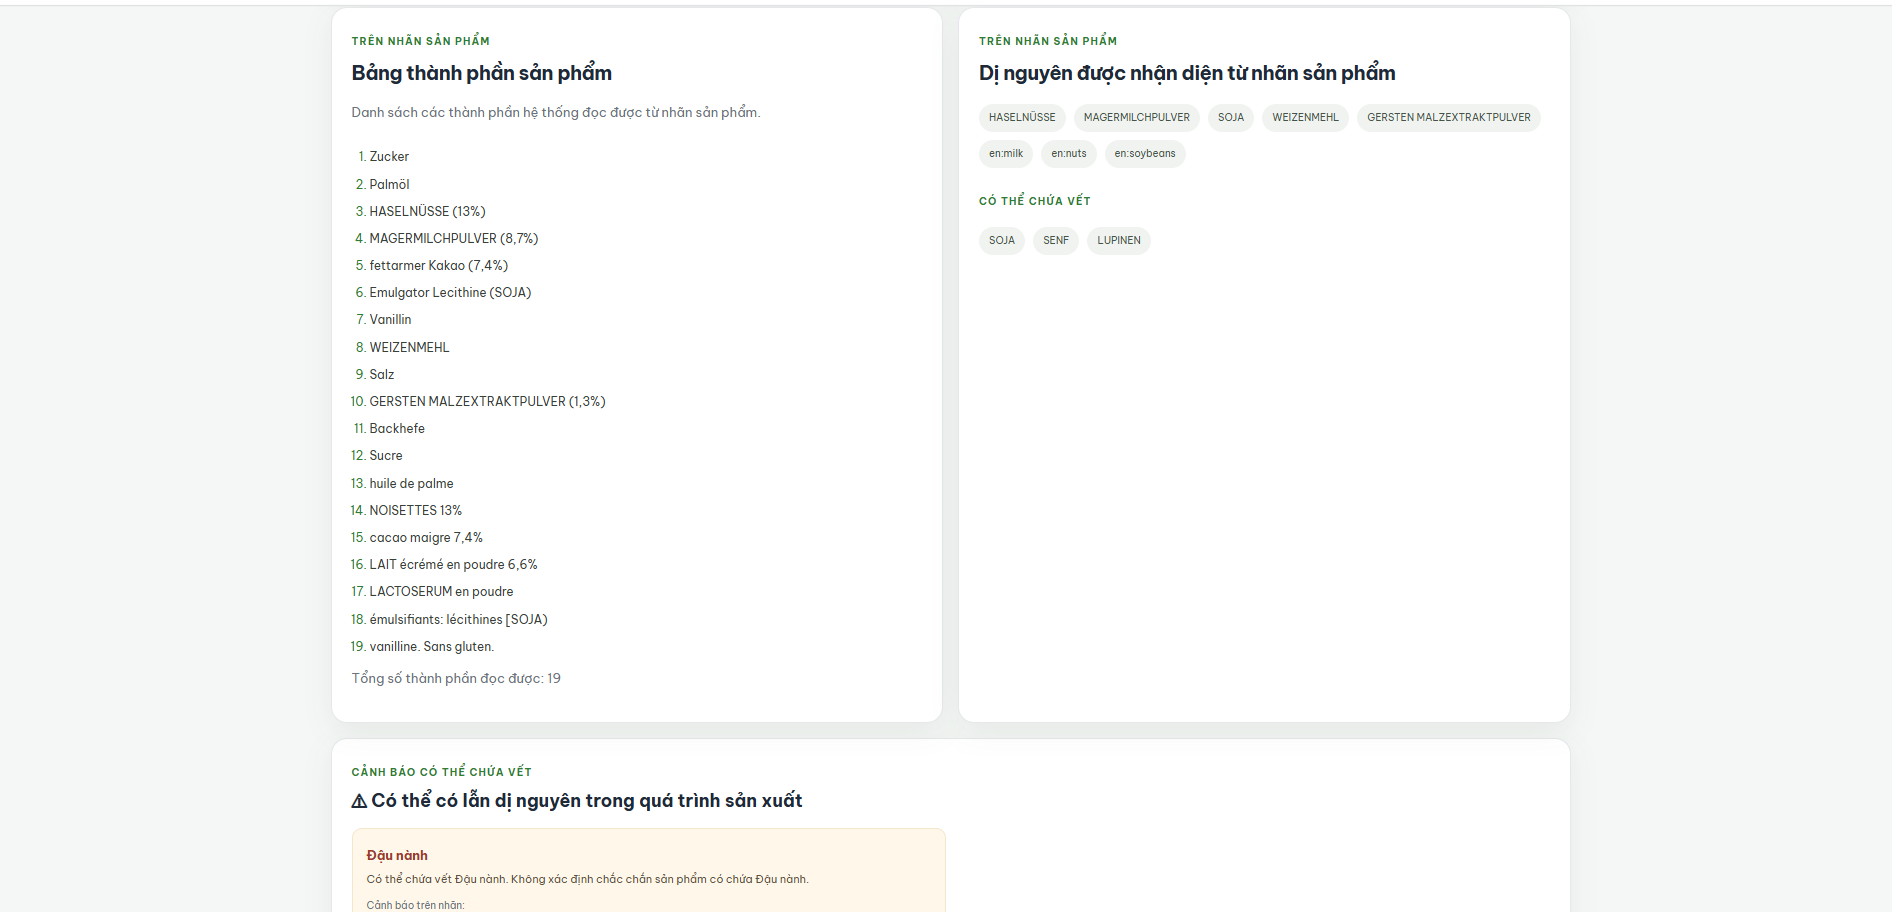
\includegraphics[width=0.90\textwidth,height=0.62\textheight,keepaspectratio]{assets/result2.png}
	\caption{Phần hiển thị chi tiết thành phần và dị nguyên}
	\label{fig:giao-dien-ket-qua-2}
\end{figure}

Hình minh họa khu vực trình bày thành phần được nhận diện và những dị nguyên có liên quan trong kết quả phân tích.


\begin{figure}[H]
	\centering
	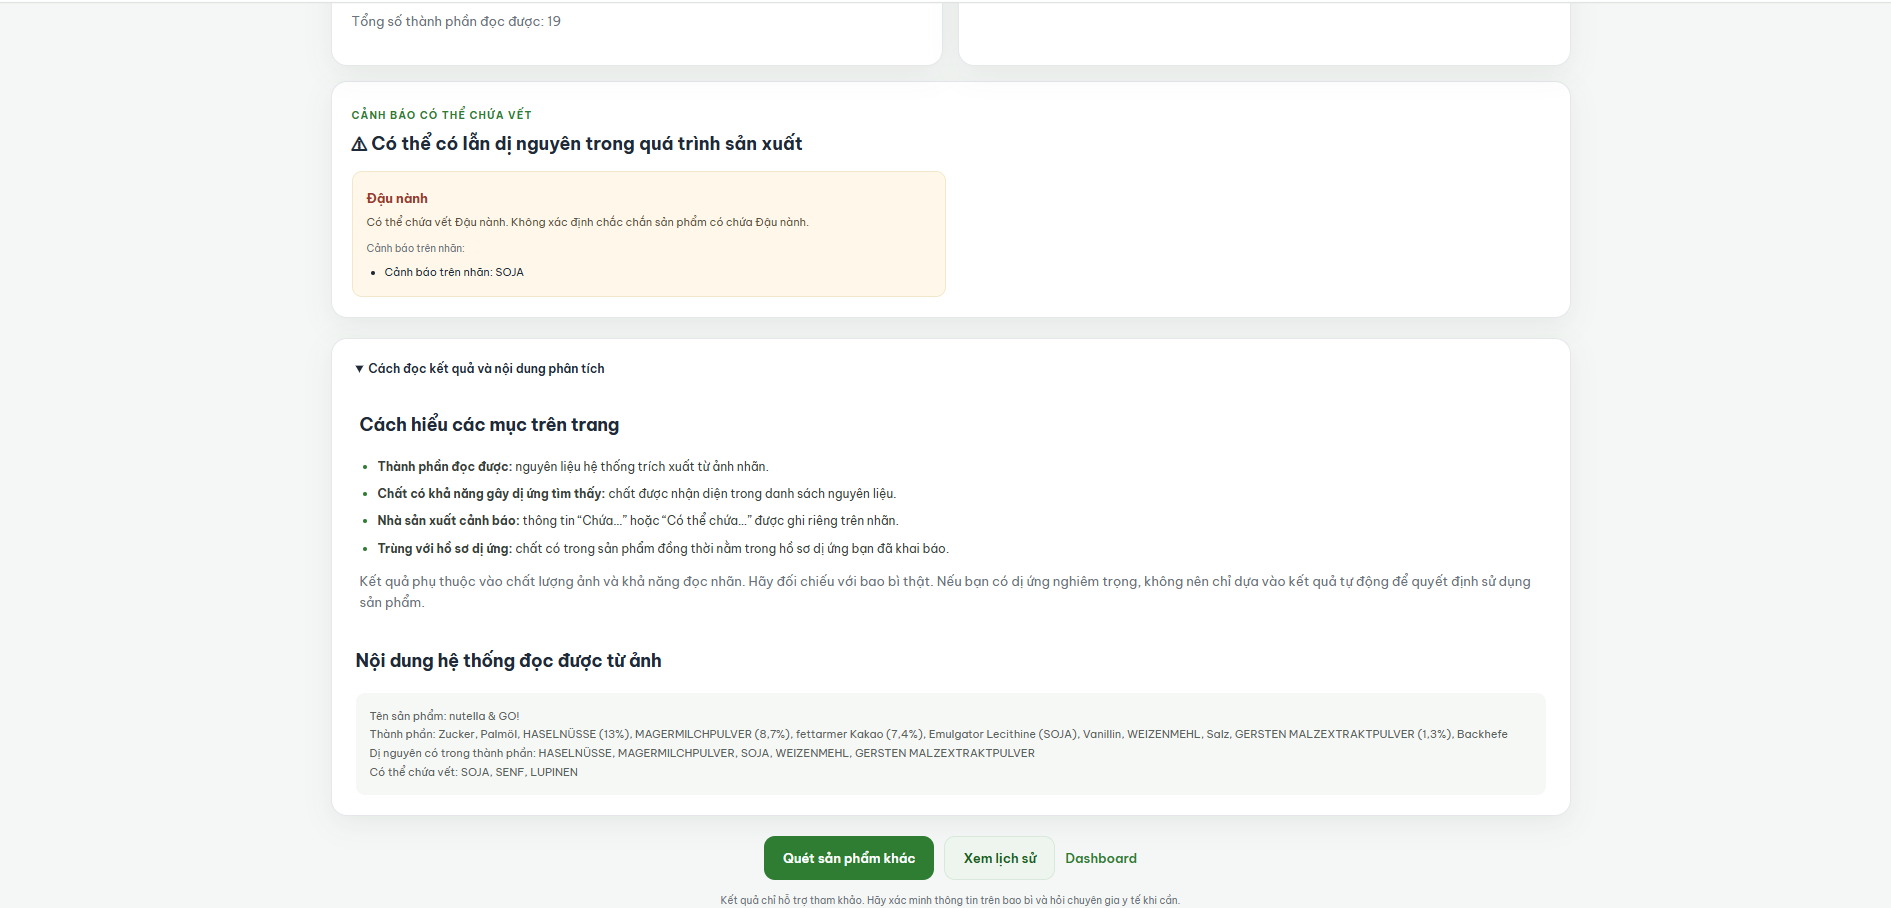
\includegraphics[width=0.90\textwidth,height=0.62\textheight,keepaspectratio]{assets/result3.png}
	\caption{Phần hiển thị chi tiết cảnh báo dị nguyên}
	\label{fig:giao-dien-ket-qua-3}
\end{figure}

Hình minh họa phần chi tiết cảnh báo, trong đó phân biệt dị nguyên có bằng chứng trong thành phần và cảnh báo có thể chứa vết.


Ba hình trên minh họa các phần khác nhau của cùng một giao diện kết quả phân tích. Việc trình bày liên tiếp giúp thể hiện đầy đủ thông tin sản phẩm, thành phần được nhận diện và các cảnh báo liên quan trong quá trình hệ thống hỗ trợ người dùng kiểm tra nhãn thực phẩm.

% =========================================================
% 3.8 GIAO DIỆN QUẢN TRỊ
% =========================================================

\Needspace{12\baselineskip}
\section{Thiết kế giao diện quản trị}

Khu vực quản trị được thiết kế dành cho tài khoản có quyền quản trị. Các màn hình minh họa thể hiện trang tổng quan, khu vực dữ liệu và chức năng xem thông tin sản phẩm. Giao diện sử dụng phong cách trình bày thống nhất với hệ thống, giúp quản trị viên thuận tiện theo dõi và thao tác.

\Needspace{9\baselineskip}
\subsection{Dashboard quản trị}

Dashboard quản trị cung cấp cái nhìn tổng quan về dữ liệu và hoạt động của hệ thống. Các thông tin được bố trí thành những khu vực riêng biệt để quản trị viên dễ theo dõi.

\begin{figure}[H]
	\centering
	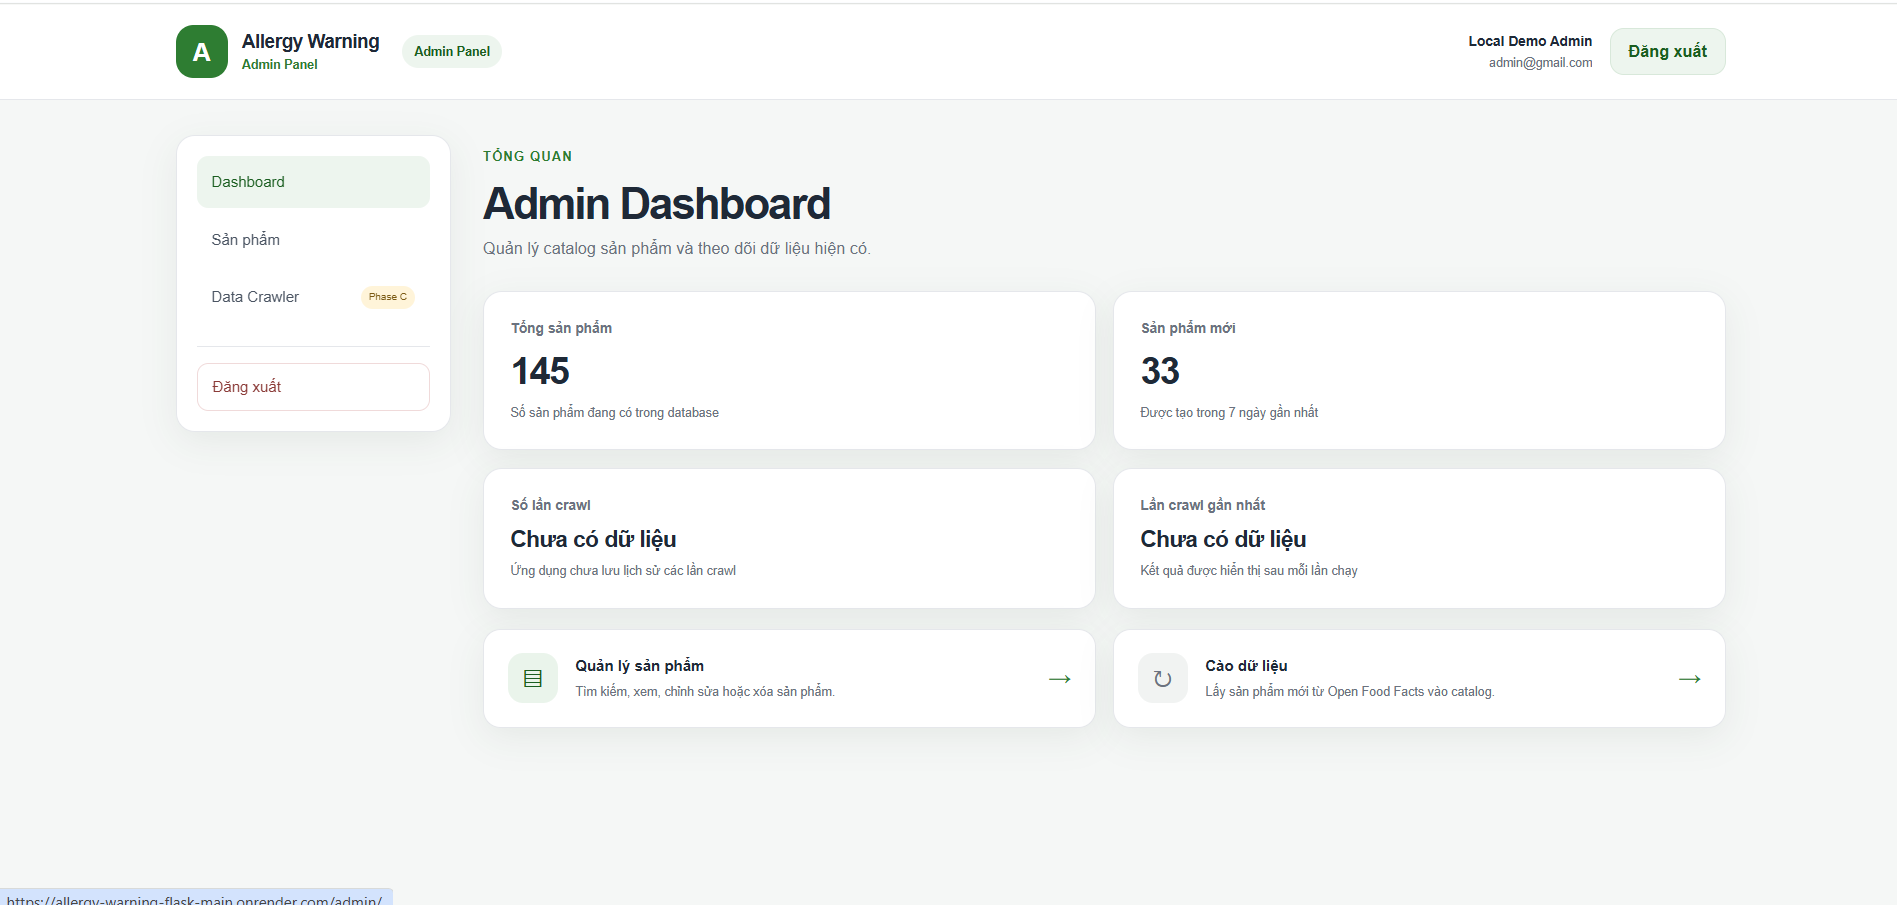
\includegraphics[width=0.95\textwidth,height=0.62\textheight,keepaspectratio]{assets/admin_dashboard.png}
	\caption{Giao diện Dashboard quản trị}
	\label{fig:admin-dashboard}
\end{figure}

Hình minh họa Dashboard quản trị, nơi hiển thị thông tin tổng quan phục vụ việc theo dõi hoạt động và dữ liệu hệ thống.


\Needspace{9\baselineskip}
\subsection{Giao diện lấy thông tin sản phẩm}

Giao diện này cho phép quản trị viên lấy thông tin sản phẩm để lưu vào hệ thống.

\begin{figure}[H]
	\centering
	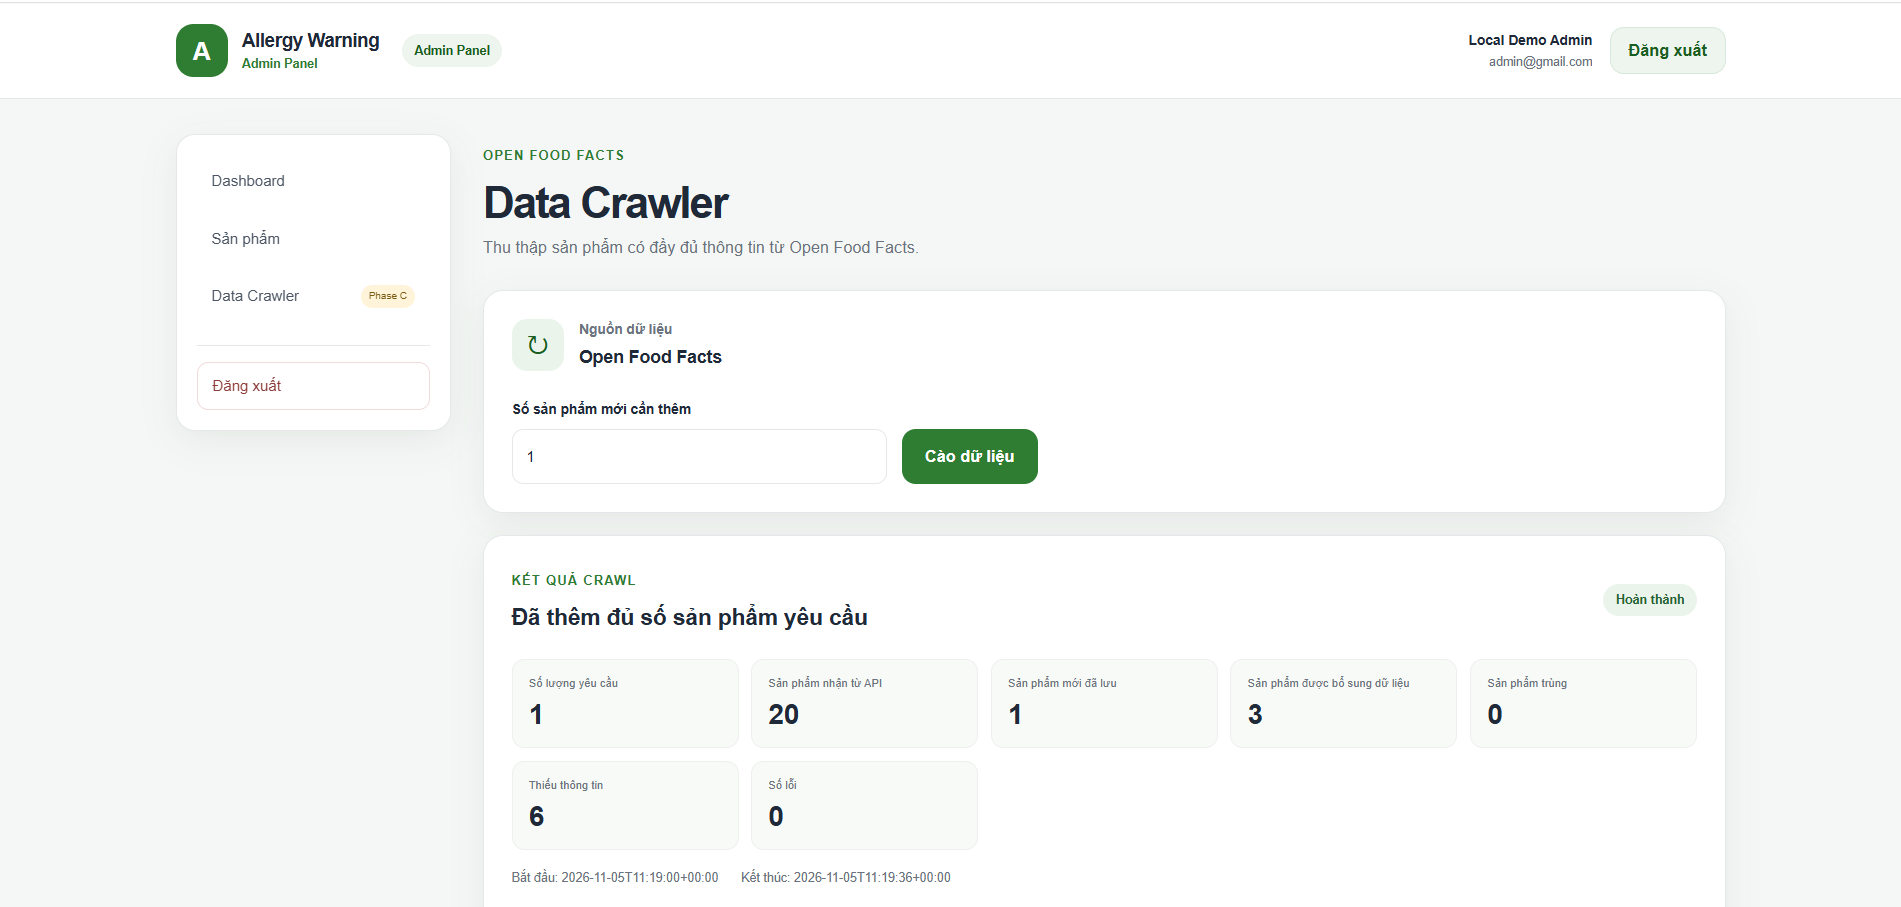
\includegraphics[width=0.95\textwidth,height=0.62\textheight,keepaspectratio]{assets/admin_data1.png}
	\caption{Giao diện thu thập dữ liệu - màn hình thứ nhất}
	\label{fig:admin-data-1}
\end{figure}

Hình minh họa màn hình đầu tiên của chức năng thu thập dữ liệu sản phẩm trong khu vực quản trị.


\begin{figure}[H]
	\centering
	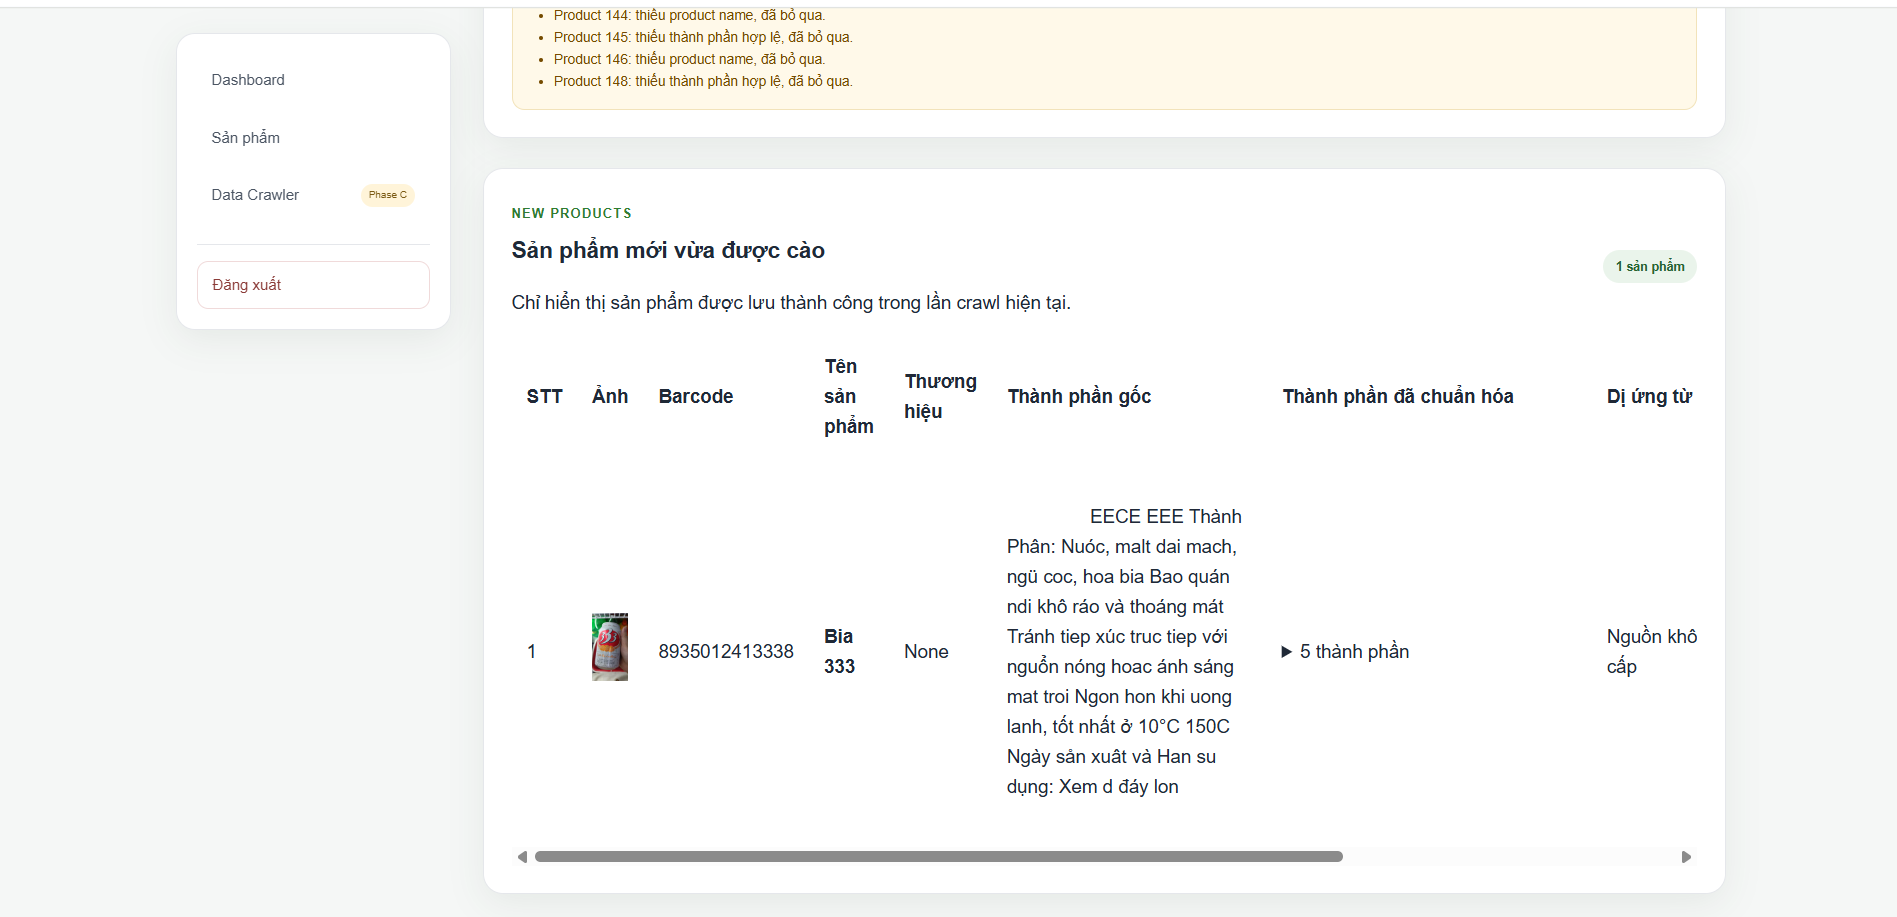
\includegraphics[width=0.95\textwidth,height=0.62\textheight,keepaspectratio]{assets/admin_data2.png}
	\caption{Giao diện thu thập dữ liệu - màn hình thứ hai}
	\label{fig:admin-data-2}
\end{figure}

Hình minh họa màn hình tiếp theo của chức năng thu thập dữ liệu, bổ sung các thao tác và thông tin phục vụ quá trình đưa dữ liệu vào hệ thống.


\Needspace{9\baselineskip}
\subsection{Giao diện quản lý sản phẩm}

Giao diện quản lý sản phẩm thể hiện khu vực quản trị danh sách sản phẩm. Quản trị viên có thể theo dõi các thông tin sản phẩm được hiển thị trong bảng dữ liệu và truy cập trang chi tiết để xem thêm thông tin tương ứng.

\begin{figure}[H]
	\centering
	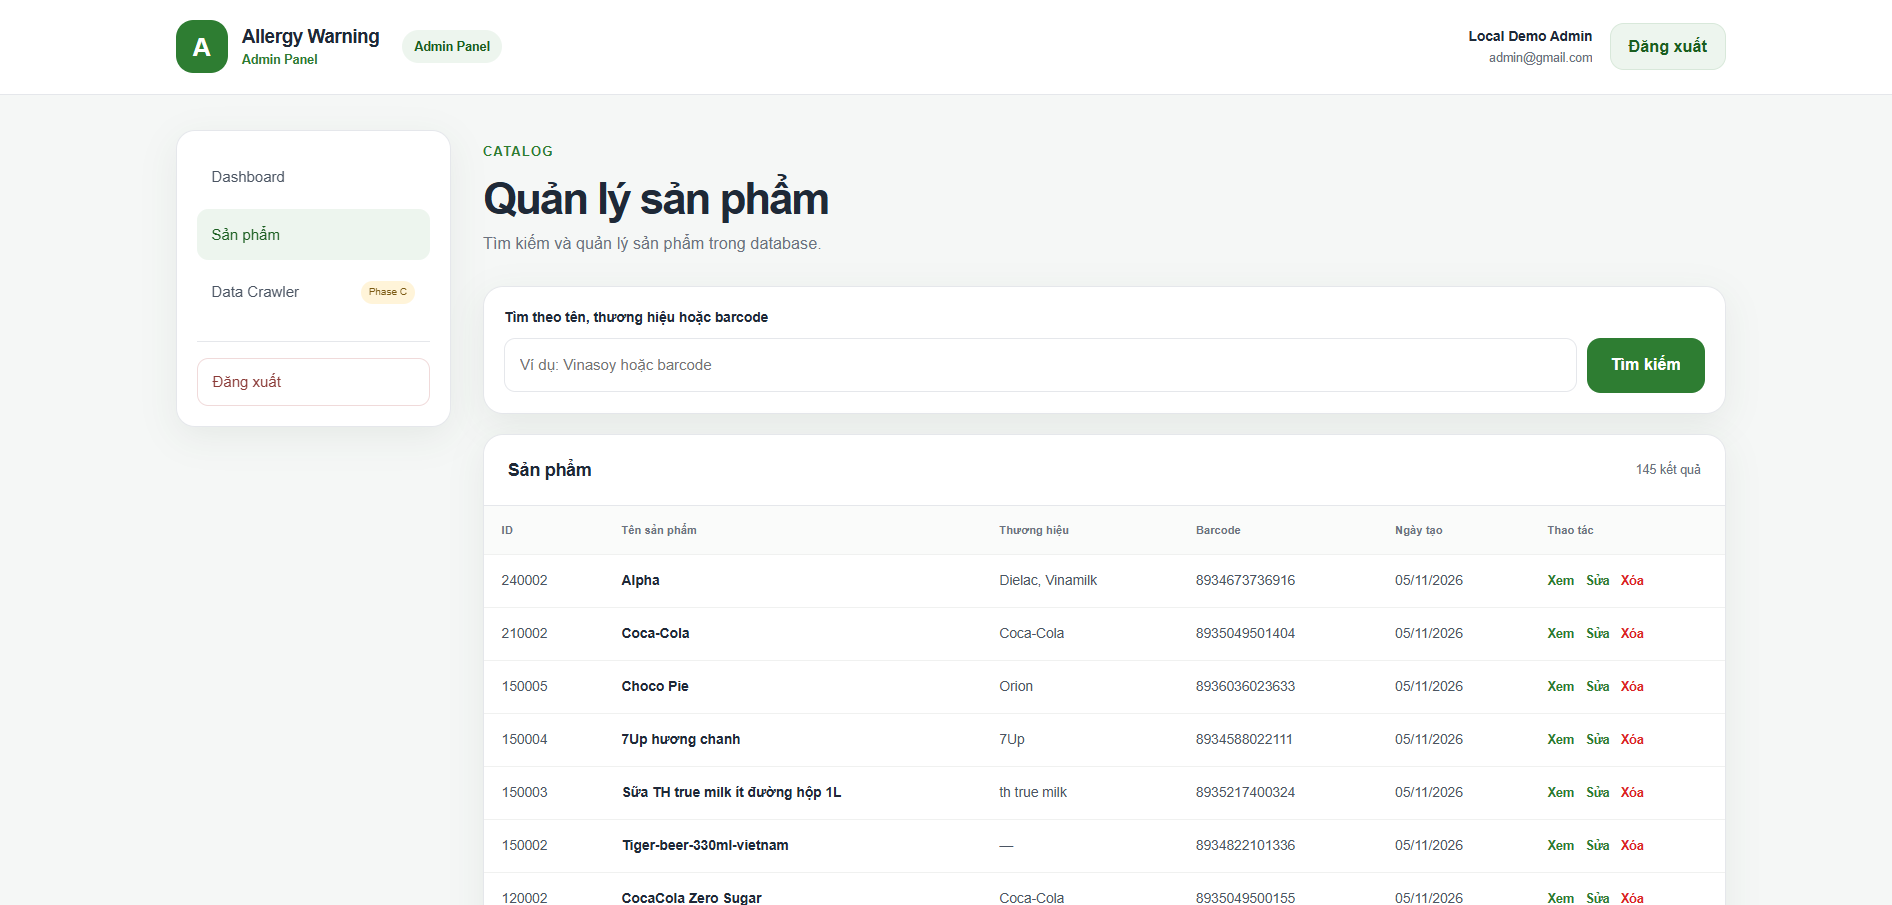
\includegraphics[width=0.95\textwidth,height=0.62\textheight,keepaspectratio]{assets/admin_product.png}
	\caption{Giao diện danh sách sản phẩm trong khu vực quản trị}
	\label{fig:admin-product}
\end{figure}

Hình minh họa danh sách sản phẩm được lưu trong hệ thống, hỗ trợ quản trị viên tra cứu và theo dõi dữ liệu.


\begin{figure}[H]
	\centering
	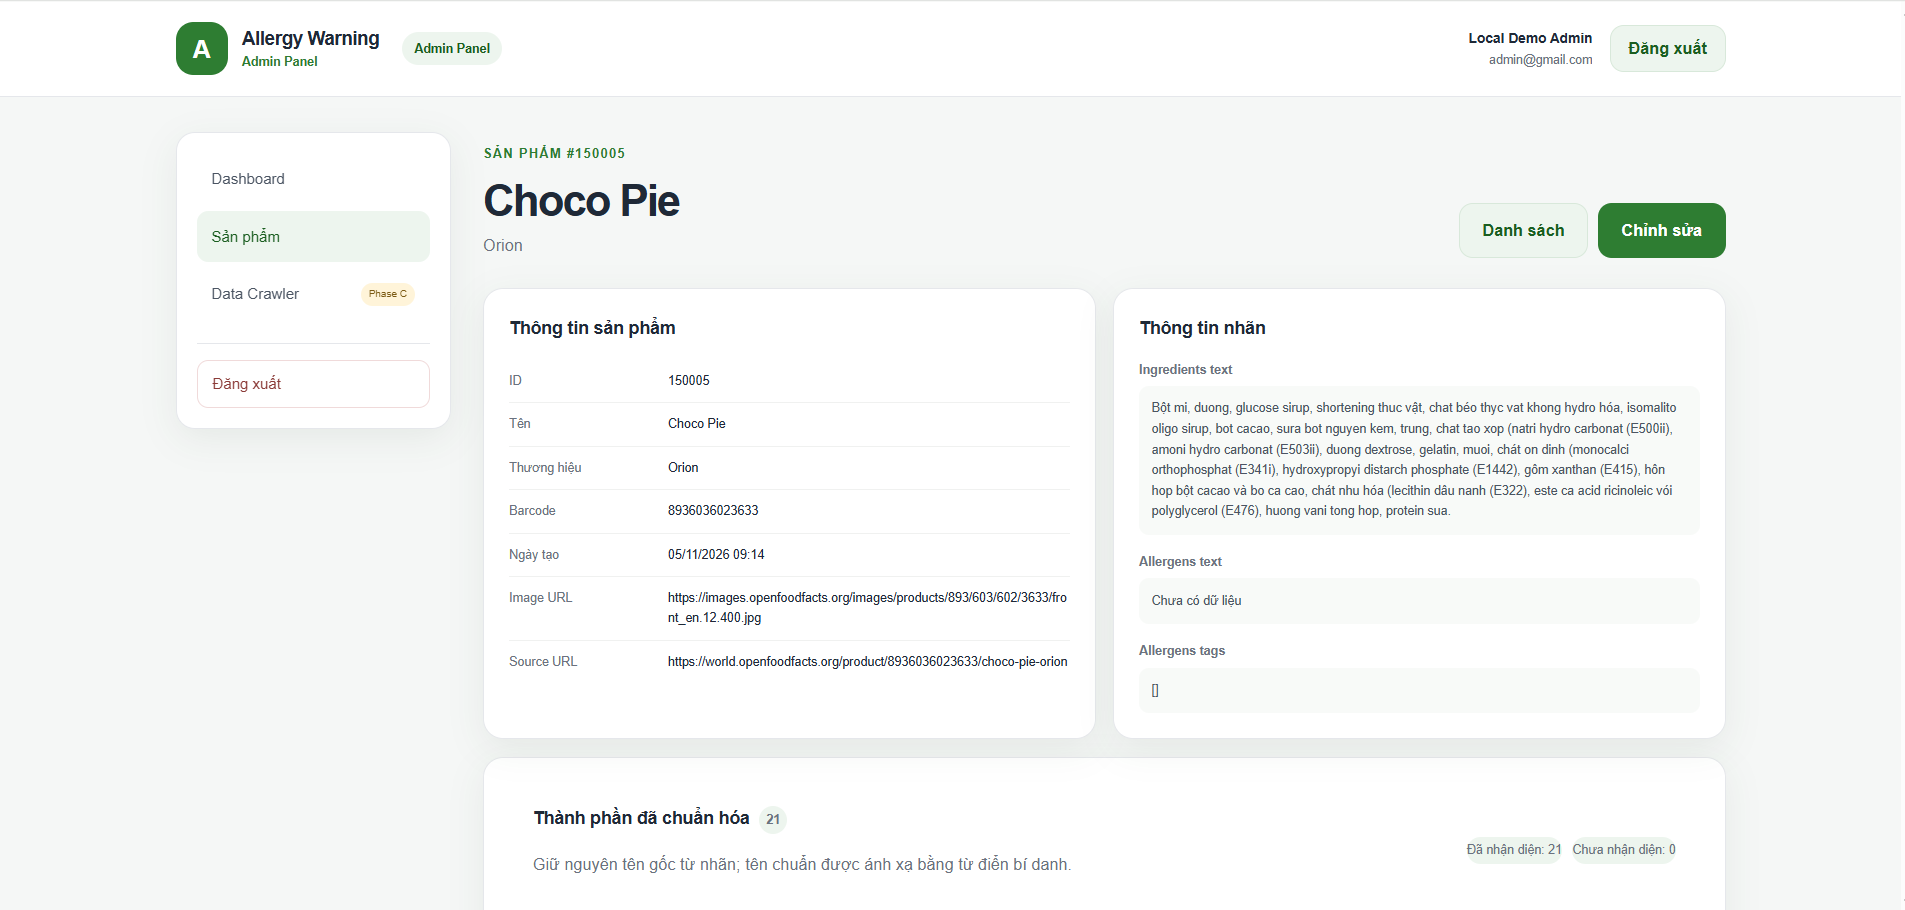
\includegraphics[width=0.95\textwidth,height=0.62\textheight,keepaspectratio]{assets/admin_productdetail.png}
	\caption{Giao diện chi tiết sản phẩm trong khu vực quản trị}
	\label{fig:admin-product-detail}
\end{figure}

Hình minh họa trang chi tiết của một sản phẩm, cung cấp thông tin cụ thể hơn so với bảng danh sách.


% =========================================================
% 3.9 KẾT LUẬN CHƯƠNG
% =========================================================

\Needspace{12\baselineskip}
\section{Kết luận chương}

Chương 3 đã trình bày quá trình phân tích bài toán, xác định đối tượng sử dụng, các yêu cầu chức năng và phi chức năng của hệ thống Allergy Warning. Từ những yêu cầu đó, chương đã mô tả kiến trúc tổng thể, vai trò của Flask, Gemini API, Cloudinary và cơ sở dữ liệu, đồng thời trình bày quy trình quét nhãn, phân tích và phân loại cảnh báo dị nguyên.

Bên cạnh đó, chương đã trình bày cấu trúc cơ sở dữ liệu \texttt{food\_allergen\_system} với sáu bảng chính gồm \texttt{user}, \texttt{allergens}, \texttt{products}, \texttt{product\_ingredients}, \texttt{user\_allergens} và \texttt{scan\_history}. Các bảng được mô tả theo trường dữ liệu và mối quan hệ nhằm làm rõ cách tổ chức thông tin phục vụ hoạt động của hệ thống.

Chương cũng trình bày các sơ đồ Use Case, kiến trúc, quy trình, ERD và các giao diện người dùng, quản trị để minh họa cách hệ thống được tổ chức và vận hành. Những nội dung về công nghệ và chức năng được mô tả theo phạm vi triển khai của hệ thống; các chức năng chưa được xây dựng không được xem là chức năng đã hoàn thiện.

	
	% CHƯƠNG 4: CÀI ĐẶT HỆ THỐNG
	% ---------------------------------------------------------------------
% CHƯƠNG 4 — CÀI ĐẶT VÀ THỬ NGHIỆM
% Hệ thống Allergy Warning
% ---------------------------------------------------------------------

\chapter{Cài đặt và thử nghiệm}
\label{ch:caidat}

\section{Môi trường triển khai}

Hệ thống Allergy Warning được xây dựng dưới dạng ứng dụng web, hỗ trợ người dùng tải ảnh nhãn thực phẩm, phân tích thành phần và đối chiếu dị nguyên với hồ sơ cá nhân. Phía máy chủ sử dụng Python và Flask để tiếp nhận yêu cầu, xử lý nghiệp vụ và kết nối các dịch vụ bên ngoài.

Cơ sở dữ liệu được triển khai trên TiDB Cloud với khả năng tương thích MySQL, dùng để lưu thông tin tài khoản, hồ sơ dị ứng, dữ liệu sản phẩm và lịch sử quét. Hình ảnh nhãn thực phẩm được lưu trữ trên Cloudinary; Gemini API hỗ trợ nhận diện nội dung trên ảnh và trích xuất thông tin sản phẩm, thành phần, dị nguyên. Ngoài ra, hệ thống sử dụng Open Food Facts làm nguồn dữ liệu tham khảo về sản phẩm.

Ứng dụng Flask được triển khai trên Render và người dùng có thể truy cập thông qua trình duyệt web. Các thông tin kết nối và khóa API được cấu hình bằng biến môi trường nhằm hạn chế đưa dữ liệu nhạy cảm trực tiếp vào mã nguồn.

\begin{table}[htbp]
	\centering
	\caption{Các công nghệ sử dụng trong hệ thống Allergy Warning}
	\label{tab:ch4-cong-nghe}
	\small
	\renewcommand{\arraystretch}{1.2}
	\begin{tabularx}{\textwidth}{|>{\raggedright\arraybackslash}p{2.8cm}|>{\raggedright\arraybackslash}p{3.2cm}|>{\raggedright\arraybackslash}X|}
		\hline
		\textbf{Thành phần} & \textbf{Công nghệ} & \textbf{Vai trò} \\ \hline
		Ngôn ngữ lập trình & Python & Xây dựng và xử lý chức năng phía máy chủ. \\ \hline
		Framework web & Flask & Tiếp nhận yêu cầu, xử lý nghiệp vụ và kết nối dịch vụ. \\ \hline
		Cơ sở dữ liệu & TiDB Cloud & Lưu tài khoản, hồ sơ dị ứng, sản phẩm và lịch sử quét. \\ \hline
		Trí tuệ nhân tạo & Gemini API & Phân tích ảnh và trích xuất thông tin trên nhãn. \\ \hline
		Lưu trữ hình ảnh & Cloudinary & Lưu ảnh nhãn thực phẩm và cung cấp URL ảnh. \\ \hline
		Nguồn dữ liệu & Open Food Facts & Cung cấp thông tin tham khảo về sản phẩm và thành phần. \\ \hline
		Giao diện & HTML, CSS, JavaScript & Xây dựng giao diện và xử lý tương tác người dùng. \\ \hline
		Triển khai & Render & Vận hành ứng dụng Flask trên môi trường trực tuyến. \\ \hline
	\end{tabularx}
\end{table}

Bảng trên tổng hợp các công nghệ chính và vai trò của từng thành phần trong hệ thống.

\subsection{Cơ sở dữ liệu}

Cơ sở dữ liệu được triển khai trên TiDB Cloud, gồm các bảng chính: \texttt{user}, \texttt{allergens}, \texttt{products}, \texttt{product\_ingredients}, \texttt{user\_allergens} và \texttt{scan\_history}. Trong đó, \texttt{user} lưu thông tin tài khoản; \texttt{allergens} quản lý danh mục dị nguyên; \texttt{products} và \texttt{product\_ingredients} lưu thông tin sản phẩm, thành phần; \texttt{user\_allergens} lưu các dị nguyên người dùng đã chọn; \texttt{scan\_history} ghi nhận kết quả những lần quét.

Ảnh nhãn được lưu trên Cloudinary thay vì lưu trực tiếp dưới dạng dữ liệu nhị phân trong cơ sở dữ liệu. Hệ thống lưu và sử dụng URL do Cloudinary trả về để truy xuất hoặc hiển thị ảnh khi cần.

\subsection{Triển khai ứng dụng}

Mã nguồn được quản lý bằng Git và lưu trữ trên GitHub. Ứng dụng Flask được triển khai trên Render; các dịch vụ TiDB Cloud, Cloudinary và Gemini API được kết nối thông qua cấu hình môi trường. Cách triển khai này tách biệt máy chủ ứng dụng, cơ sở dữ liệu và dịch vụ lưu trữ ảnh, đồng thời giúp quản lý cấu hình của từng dịch vụ độc lập.

\section{Cài đặt các chức năng chính}

\subsection{Đăng ký và đăng nhập}

Chức năng đăng ký cho phép người dùng tạo tài khoản thông qua biểu mẫu nhập thông tin. Hệ thống kiểm tra dữ liệu đầu vào trước khi lưu tài khoản vào cơ sở dữ liệu. Chức năng đăng nhập xác thực thông tin tài khoản; nếu hợp lệ, người dùng được truy cập các chức năng tương ứng, ngược lại hệ thống hiển thị thông báo phù hợp. Mật khẩu được lưu dưới dạng đã băm nhằm bảo vệ thông tin tài khoản.

\subsection{Quản lý hồ sơ dị ứng}

Người dùng có thể lựa chọn những nhóm dị nguyên cần quan tâm từ danh mục được hệ thống quản lý. Các lựa chọn được lưu thông qua bảng \texttt{user\_allergens} và liên kết với tài khoản tương ứng. Khi phân tích sản phẩm, hệ thống sử dụng hồ sơ này để đối chiếu với những dị nguyên nhận diện được trên nhãn.

\subsection{Quét và lưu trữ ảnh nhãn thực phẩm}

Người dùng chọn ảnh nhãn thực phẩm từ thiết bị và gửi lên hệ thống. Flask tiếp nhận, kiểm tra tệp đầu vào, sau đó tải ảnh lên Cloudinary. Khi tải lên thành công, Cloudinary trả về URL ảnh để hệ thống sử dụng trong quá trình phân tích và lưu lịch sử. Ảnh mờ, thiếu sáng hoặc không thể đọc rõ nội dung có thể ảnh hưởng đến kết quả nhận diện.

\subsection{Phân tích nội dung nhãn bằng Gemini API}

Sau khi nhận ảnh, máy chủ gửi yêu cầu đến Gemini API để hỗ trợ đọc nội dung nhãn. Kết quả trích xuất có thể gồm tên sản phẩm, thương hiệu, mã vạch, danh sách thành phần và thông tin cảnh báo dị nguyên. Flask tiếp nhận dữ liệu trả về, kiểm tra và tổ chức thành các trường thông tin phục vụ những bước xử lý tiếp theo.

Kết quả phụ thuộc vào chất lượng ảnh và nội dung thể hiện trên bao bì. Vì vậy, hệ thống cần xử lý trường hợp dữ liệu thiếu, không hợp lệ hoặc dịch vụ AI không phản hồi; không sử dụng dữ liệu chưa được xác nhận để đưa ra kết luận cảnh báo.

\subsection{Tra cứu dữ liệu sản phẩm}

Open Food Facts được sử dụng làm nguồn dữ liệu tham khảo để tra cứu thông tin sản phẩm. Dữ liệu có thể bao gồm mã vạch, tên sản phẩm, thương hiệu, thành phần và dị nguyên. Hệ thống kiểm tra thông tin nhận được trước khi sử dụng hoặc bổ sung vào cơ sở dữ liệu. Do dữ liệu của từng sản phẩm có thể chưa đầy đủ, thông tin thiếu không được xem là bằng chứng cho thấy sản phẩm không chứa dị nguyên.

\subsection{Chuẩn hóa và đối chiếu dị nguyên}

Thông tin thành phần sau khi trích xuất được chuẩn hóa nhằm thống nhất cách viết, loại bỏ khoảng trắng dư thừa và xử lý những tên gọi tương đương đã có trong dữ liệu tham chiếu. Việc chuẩn hóa phải giữ nguyên ý nghĩa của nội dung trên nhãn, đặc biệt là các cụm từ thể hiện cảnh báo của nhà sản xuất.

Sau đó, hệ thống đối chiếu thành phần và thông tin cảnh báo với danh mục dị nguyên. Kết quả được phân biệt thành dị nguyên nhận diện từ thành phần, dị nguyên được nhà sản xuất cảnh báo riêng và dị nguyên có thể chứa vết. Các dị nguyên nhận diện được tiếp tục so sánh với hồ sơ cá nhân để xác định nội dung trùng khớp.

\subsection{Hiển thị kết quả và lưu lịch sử quét}

Kết quả phân tích được trình bày theo từng nhóm thông tin, gồm thông tin sản phẩm, thành phần nhận diện được, dị nguyên liên quan và trạng thái đối chiếu với hồ sơ dị ứng. Người dùng có thể xem lại những lần phân tích trước đó tại chức năng lịch sử quét. Mỗi bản ghi được liên kết với tài khoản tương ứng và lưu trong bảng \texttt{scan\_history}.

Kết quả phân tích chỉ có tính chất hỗ trợ tham khảo, không thay thế việc kiểm tra nhãn sản phẩm thực tế hoặc tư vấn chuyên môn y tế.

\section{Quy trình hoạt động của hệ thống}

Quy trình quét nhãn bắt đầu khi người dùng chọn và gửi ảnh lên hệ thống. Flask kiểm tra ảnh đầu vào, tải ảnh lên Cloudinary và gửi ảnh đến Gemini API để trích xuất thông tin. Dữ liệu nhận được tiếp tục được chuẩn hóa, đối chiếu với danh mục dị nguyên và hồ sơ của người dùng. Cuối cùng, hệ thống tổng hợp kết quả, lưu lịch sử quét vào TiDB Cloud và hiển thị thông tin trên giao diện.

\begin{enumerate}
	\item Người dùng chọn ảnh nhãn thực phẩm và gửi lên hệ thống.
	\item Flask kiểm tra định dạng và dữ liệu ảnh đầu vào.
	\item Ảnh được tải lên Cloudinary để nhận URL lưu trữ.
	\item Gemini API phân tích ảnh và trích xuất thông tin trên nhãn.
	\item Flask kiểm tra, chuẩn hóa dữ liệu thành phần và cảnh báo.
	\item Hệ thống đối chiếu dị nguyên với dữ liệu và hồ sơ người dùng.
	\item Kết quả phân tích được tổng hợp và lưu vào lịch sử quét.
	\item Giao diện hiển thị kết quả để người dùng kiểm tra.
\end{enumerate}

Quy trình trên thể hiện luồng xử lý chính từ lúc tiếp nhận ảnh đến khi trả kết quả. Nếu ảnh không hợp lệ, dịch vụ bên ngoài gặp lỗi hoặc dữ liệu trích xuất không đáp ứng yêu cầu, hệ thống cần thông báo và không hiển thị kết luận chưa có căn cứ.

\section{Giao diện hệ thống}

Giao diện Allergy Warning được xây dựng bằng HTML, CSS và JavaScript, hỗ trợ người dùng thao tác với các chức năng đăng nhập, quản lý hồ sơ dị ứng, quét nhãn, xem kết quả và tra cứu lịch sử.

\subsection{Giao diện đăng nhập và đăng ký}

Giao diện đăng nhập cho phép người dùng nhập thông tin tài khoản để truy cập hệ thống. Giao diện đăng ký cung cấp biểu mẫu tạo tài khoản mới và thông báo khi dữ liệu nhập vào chưa hợp lệ.

% Chèn hình ảnh giao diện đăng nhập và đăng ký tại đây nếu có.

\subsection{Giao diện trang chủ và hồ sơ dị ứng}

Trang chủ cung cấp các chức năng chính để người dùng truy cập. Tại hồ sơ dị ứng, người dùng có thể xem và lựa chọn những nhóm dị nguyên cần quan tâm.

% Chèn hình ảnh giao diện trang chủ và hồ sơ dị ứng tại đây nếu có.

\subsection{Giao diện quét nhãn và kết quả phân tích}

Giao diện quét nhãn cho phép người dùng tải ảnh thực phẩm lên để phân tích. Sau khi xử lý, trang kết quả hiển thị thông tin sản phẩm, thành phần được nhận diện, dị nguyên liên quan và cảnh báo đối chiếu với hồ sơ cá nhân.

% Chèn hình ảnh giao diện quét nhãn và kết quả phân tích tại đây nếu có.

\subsection{Giao diện lịch sử quét}

Giao diện lịch sử quét hiển thị những lần phân tích đã được lưu theo tài khoản. Người dùng có thể xem lại thông tin của từng lần quét để tham khảo.

% Chèn hình ảnh giao diện lịch sử quét tại đây nếu có.

\section{Kiểm thử hệ thống}

\subsection{Mục tiêu kiểm thử}

Kiểm thử nhằm đánh giá hoạt động của các chức năng chính, tập trung vào đăng nhập, quản lý hồ sơ dị ứng, tải ảnh, phân tích nhãn, đối chiếu dị nguyên, hiển thị kết quả và lưu lịch sử. Các trường hợp kiểm thử bao gồm dữ liệu hợp lệ, dữ liệu không hợp lệ và những tình huống lỗi có thể phát sinh.

\subsection{Các trường hợp kiểm thử}

Bảng~\ref{tab:ch4-testcases} trình bày một số trường hợp kiểm thử chính. Kết quả thực tế cần được cập nhật sau khi thực hiện kiểm thử trên ứng dụng.

\begin{longtable}{|>{\centering\arraybackslash}p{0.8cm}|>{\raggedright\arraybackslash}p{3.1cm}|>{\raggedright\arraybackslash}p{8.2cm}|>{\raggedright\arraybackslash}p{2.2cm}|}
	\caption{Các trường hợp kiểm thử hệ thống Allergy Warning}
	\label{tab:ch4-testcases}\\
	\hline
	\textbf{Mã} & \textbf{Trường hợp kiểm thử} & \textbf{Kết quả mong đợi} & \textbf{Kết quả thực tế} \\ \hline
	\endfirsthead
	
	\multicolumn{4}{c}{\tablename\ \thetable{} -- tiếp theo}\\
	\hline
	\textbf{Mã} & \textbf{Trường hợp kiểm thử} & \textbf{Kết quả mong đợi} & \textbf{Kết quả thực tế} \\ \hline
	\endhead
	
	\hline
	\multicolumn{4}{r}{\textit{Bảng tiếp tục ở trang sau}}\\
	\endfoot
	
	\hline
	\endlastfoot
	TC01 & Đăng ký với thông tin hợp lệ & Tạo tài khoản và lưu thông tin thành công. & Pass. \\ \hline
	TC02 & Đăng ký với email đã tồn tại & Từ chối tạo tài khoản và thông báo email đã được sử dụng. & Pass. \\ \hline
	TC03 & Đăng ký khi bỏ trống trường bắt buộc & Hiển thị thông báo yêu cầu nhập đầy đủ thông tin. & Pass. \\ \hline
	TC04 & Đăng ký với email sai định dạng & Không chấp nhận dữ liệu email không hợp lệ. &Pass. \\ \hline
	TC05 & Đăng nhập với thông tin hợp lệ & Xác thực tài khoản và truy cập hệ thống thành công. & Pass. \\ \hline
	TC06 & Đăng nhập với mật khẩu không đúng & Từ chối đăng nhập và hiển thị thông báo phù hợp. & Pass. \\ \hline
	TC07 & Đăng nhập khi bỏ trống email hoặc mật khẩu & Yêu cầu người dùng nhập đầy đủ thông tin. & Pass. \\ \hline
	TC08 & Đăng xuất khỏi hệ thống & Kết thúc phiên đăng nhập và chuyển về trang phù hợp. & Pass. \\ \hline
	TC09 & Xem thông tin hồ sơ cá nhân & Hiển thị đúng thông tin của tài khoản đang đăng nhập. &Pass. \\ \hline
	TC10 & Cập nhật thông tin hồ sơ cá nhân & Lưu và hiển thị thông tin mới sau khi cập nhật. & Pass. \\ \hline
	TC11 & Xem danh sách dị nguyên & Hiển thị danh mục dị nguyên có trong hệ thống. & Pass. \\ \hline
	TC12 & Chọn dị nguyên trong hồ sơ cá nhân & Lưu đúng các dị nguyên người dùng đã lựa chọn. &Pass. \\ \hline
	TC13 & Bỏ chọn dị nguyên đã lưu & Cập nhật hồ sơ và loại bỏ lựa chọn tương ứng. & Pass. \\ \hline
	TC14 & Tải ảnh nhãn thực phẩm hợp lệ & Tiếp nhận ảnh và chuyển sang bước lưu trữ, phân tích. & Pass. \\ \hline
	TC15 & Không chọn ảnh khi thực hiện quét & Hiển thị yêu cầu chọn ảnh trước khi tiếp tục. & Pass. \\ \hline
	TC16 & Tải tệp không phải định dạng ảnh hỗ trợ & Từ chối tệp và thông báo định dạng không hợp lệ. &Pass. \\ \hline
	TC17 & Tải ảnh vượt quá dung lượng cho phép & Từ chối ảnh hoặc thông báo giới hạn dung lượng. & Pass. \\ \hline
	TC18 & Tải ảnh lên Cloudinary thành công & Nhận URL ảnh và sử dụng URL trong quá trình phân tích. &Pass. \\ \hline
	TC19 & Cloudinary không phản hồi hoặc tải ảnh thất bại & Thông báo lỗi và không tiếp tục phân tích bằng URL không hợp lệ. & Pass. \\ \hline
	TC20 & Phân tích ảnh nhãn có nội dung rõ ràng & Gemini API trích xuất thông tin sản phẩm và nội dung nhãn. & Pass. \\ \hline
	TC21 & Phân tích ảnh mờ hoặc thiếu sáng & Thông báo khi dữ liệu nhận diện không đầy đủ hoặc không đáng tin cậy. & Pass. \\ \hline
	TC22 & Gemini API không phản hồi & Thông báo lỗi dịch vụ và xử lý phù hợp, không làm gián đoạn ứng dụng. & Pass. \\ \hline
	TC23 & Nhãn có thông tin mã vạch & Trích xuất mã vạch nếu thông tin hiển thị đủ rõ trên ảnh. &Pass. \\ \hline
	TC24 & Tra cứu sản phẩm bằng mã vạch có trong cơ sở dữ liệu & Trả về thông tin sản phẩm tương ứng với mã vạch. & Pass. \\ \hline
	TC25 & Tra cứu sản phẩm không tìm thấy mã vạch & Tiếp tục xử lý theo phương thức tra cứu phù hợp hoặc thông báo không tìm thấy. & Pass. \\ \hline
	TC26 & Sản phẩm có thông tin thành phần trong cơ sở dữ liệu & Truy xuất danh sách thành phần liên quan đến sản phẩm. & Pass. \\ \hline
	TC27 & Thành phần có tên gọi tương đương & Chuẩn hóa và đối chiếu theo dữ liệu tên gọi đã được hỗ trợ. & Pass. \\ \hline
	TC28 & Thành phần có tên gần giống nhưng khác ý nghĩa & Không kết luận nhầm dị nguyên chỉ dựa trên chuỗi ký tự tương tự. & Pass. \\ \hline
	TC29 & Thành phần chứa dị nguyên người dùng đã chọn & Hiển thị dị nguyên trùng với hồ sơ dị ứng của người dùng. & Pass. \\ \hline
	TC30 & Thành phần chứa dị nguyên không có trong hồ sơ cá nhân & Hiển thị thông tin dị nguyên nhận diện được nhưng không đánh dấu trùng hồ sơ. & Pass. \\ \hline
	TC31 & Nhãn có cảnh báo ``có thể chứa'' hoặc ``có thể chứa vết'' & Hiển thị riêng cảnh báo có thể chứa vết, không gộp với thành phần thực tế. & Pass. \\ \hline
	TC32 & Nhãn không thể hiện thông tin dị nguyên rõ ràng & Không tự kết luận sản phẩm an toàn; hiển thị trạng thái thiếu thông tin phù hợp. & Pass. \\ \hline
	TC33 & Xem kết quả phân tích sau khi quét & Hiển thị thông tin sản phẩm, thành phần và cảnh báo đã xử lý. & Pass. \\ \hline
	TC34 & Lưu kết quả quét vào lịch sử & Tạo bản ghi lịch sử kèm thông tin kết quả và tài khoản tương ứng. & Pass. \\ \hline
	TC35 & Xem lịch sử quét của tài khoản & Chỉ hiển thị lịch sử thuộc tài khoản đang đăng nhập. & Pass. \\ \hline
	TC36 & Xem chi tiết một lần quét trong lịch sử & Hiển thị đúng thông tin của lần quét được chọn. & Pass. \\ \hline
	TC37 & Người dùng chưa đăng nhập truy cập chức năng yêu cầu tài khoản & Chuyển đến trang đăng nhập hoặc từ chối truy cập theo thiết kế. &Pass. \\ \hline
	TC38 & Hai tài khoản xem lịch sử quét riêng biệt & Mỗi tài khoản chỉ xem được dữ liệu lịch sử của chính mình. & Pass. \\ \hline
\end{longtable}

Bảng trên mô tả kết quả mong đợi của các trường hợp kiểm thử. Nhóm cần ghi nhận kết quả thực tế và đánh dấu đạt hoặc không đạt sau mỗi lần thực hiện.

\subsection{Đánh giá kết quả kiểm thử}

Đối với chức năng phân tích nhãn, kết quả nhận diện cần được so sánh với nội dung trên ảnh gốc để kiểm tra khả năng trích xuất tên sản phẩm, thành phần và cảnh báo. Đối với chức năng đối chiếu, cần kiểm tra dị nguyên được phát hiện có phù hợp với dữ liệu nhãn và hồ sơ người dùng hay không.

\Needspace{4\baselineskip}
Ngoài ra, cần kiểm tra dữ liệu lịch sử được lưu trong TiDB Cloud và URL ảnh do Cloudinary cung cấp. Những lỗi phát sinh trong quá trình kiểm thử cần được ghi nhận để phục vụ việc điều chỉnh hệ thống.

\Needspace{6\baselineskip}
\subsection{Tổng hợp kết quả kiểm thử}

Bảng~\ref{tab:ch4-test-summary} được sử dụng để tổng hợp kết quả sau khi hoàn thành kiểm thử.

\begin{table}[htbp]
	\centering
	\caption{Tổng hợp kết quả kiểm thử}
	\label{tab:ch4-test-summary}
	\small
	\renewcommand{\arraystretch}{1.2}
	\begin{tabularx}{0.9\textwidth}{|>{\raggedright\arraybackslash}p{5cm}|>{\raggedright\arraybackslash}X|}
		\hline
		\textbf{Nội dung} & \textbf{Kết quả ghi nhận} \\ \hline
		Tổng số trường hợp kiểm thử & Cập nhật theo thực tế. \\ \hline
		Số trường hợp đạt & Cập nhật theo thực tế. \\ \hline
		Số trường hợp không đạt & Cập nhật theo thực tế. \\ \hline
		Lỗi phát hiện và hướng khắc phục & Ghi nhận theo kết quả kiểm thử. \\ \hline
	\end{tabularx}
\end{table}

\section{Hạn chế và hướng phát triển}

\subsection{Hạn chế}

Khả năng phân tích phụ thuộc vào chất lượng ảnh và nội dung nhãn. Ảnh mờ, thiếu sáng hoặc chữ nhỏ có thể khiến hệ thống nhận diện thiếu hoặc sai thông tin. Bên cạnh đó, phạm vi dữ liệu dị nguyên và các biến thể tên thành phần chưa thể bao quát toàn bộ sản phẩm thực tế.

Hệ thống còn phụ thuộc vào Gemini API, Cloudinary và Open Food Facts nên có thể bị ảnh hưởng bởi kết nối mạng, giới hạn dịch vụ hoặc dữ liệu bên ngoài chưa đầy đủ. Vì vậy, kết quả phân tích cần được người dùng kiểm tra lại với bao bì thực phẩm thực tế.

\subsection{Hướng phát triển}

Trong thời gian tới, hệ thống có thể được cải thiện theo các hướng: nâng cao khả năng xử lý ảnh đầu vào; mở rộng danh mục dị nguyên và tên gọi tương đương; bổ sung căn cứ cho từng cảnh báo; cải thiện xử lý lỗi khi dịch vụ bên ngoài không phản hồi; cập nhật dữ liệu sản phẩm và mở rộng kiểm thử với nhiều loại nhãn khác nhau.

\section{Kết luận chương}

Chương 4 đã trình bày môi trường triển khai, các công nghệ sử dụng và cách cài đặt những chức năng chính của hệ thống Allergy Warning. Nội dung tập trung vào quy trình tiếp nhận và lưu trữ ảnh, phân tích nhãn bằng Gemini API, chuẩn hóa thành phần, đối chiếu dị nguyên và hiển thị kết quả. Chương cũng đề cập đến giao diện, kiểm thử, những hạn chế và hướng phát triển của hệ thống.

	
	% CHƯƠNG 5: KẾT QUẢ VÀ ĐÁNH GIÁ
	% =====================================================================
% CHƯƠNG 5: KẾT QUẢ VÀ ĐÁNH GIÁ
% ĐỀ TÀI: XÂY DỰNG HỆ THỐNG ĐỌC NHÃN MÁC VÀ CẢNH BÁO DỊ ỨNG THỰC PHẨM
% =====================================================================

\chapter{Kết quả và đánh giá}
\label{ch:ketqua}

\section{Kết quả đạt được}

\subsection{Kết quả xây dựng hệ thống}

Hệ thống Allergy Warning được xây dựng nhằm hỗ trợ người dùng đọc
thông tin trên nhãn thực phẩm và nhận biết các thành phần liên quan
đến dị ứng. Các chức năng chính gồm:

\begin{itemize}
	\item Đăng ký, đăng nhập và quản lý hồ sơ cá nhân.
	\item Thiết lập hồ sơ dị ứng và lựa chọn các dị nguyên quan tâm.
	\item Tải ảnh nhãn thực phẩm để thực hiện phân tích.
	\item Sử dụng Gemini API để nhận diện và trích xuất thông tin trên nhãn.
	\item Chuẩn hóa thành phần, đối chiếu với dữ liệu dị nguyên và hồ sơ người dùng.
	\item Hiển thị cảnh báo, lưu và tra cứu lịch sử quét.
\end{itemize}

Hệ thống sử dụng Flask làm máy chủ, TiDB Cloud lưu trữ dữ liệu,
Cloudinary lưu trữ hình ảnh và Gemini API hỗ trợ phân tích nhãn.
Open Food Facts được sử dụng làm nguồn dữ liệu tham khảo; ứng dụng
được triển khai trên Render.

\subsection{Kết quả phân tích và cảnh báo}

Quy trình phân tích gồm tiếp nhận ảnh, lưu ảnh trên Cloudinary,
gửi ảnh đến Gemini API, chuẩn hóa thông tin và đối chiếu thành phần
với dữ liệu dị nguyên. Kết quả được tổng hợp để hiển thị cho người dùng.

Hệ thống phân biệt thành phần được liệt kê trên nhãn với cảnh báo
về khả năng chứa vết dị nguyên. Đồng thời, hệ thống thể hiện riêng
dị nguyên được nhận diện và dị nguyên trùng với hồ sơ cá nhân.
Kết quả chỉ có tính chất tham khảo, không khẳng định sản phẩm an toàn
tuyệt đối.

\section{Đánh giá các chức năng}

Việc đánh giá tập trung vào khả năng hoạt động và tính phù hợp của
kết quả ở các chức năng chính.

\subsection{Quản lý tài khoản và hồ sơ dị ứng}

Kiểm tra khả năng đăng ký, đăng nhập, cập nhật hồ sơ và lưu lựa chọn
dị nguyên. Dữ liệu hồ sơ và lịch sử quét cần được truy xuất đúng theo
tài khoản đang đăng nhập.

\subsection{Phân tích hình ảnh và nhận diện nội dung}

Đối chiếu thông tin Gemini API trả về với nhãn gốc. Ảnh rõ, đủ sáng
giúp quá trình nhận diện thuận lợi hơn; ảnh mờ, nghiêng hoặc có chữ
nhỏ có thể làm thiếu hoặc sai thông tin.

\subsection{Đối chiếu dị nguyên}

Kiểm tra khả năng chuẩn hóa tên thành phần và phát hiện dị nguyên.
Cần chú ý các tên gọi tương đương, những thành phần gần giống nhau
và trường hợp dị nguyên được nhận diện nhưng không nằm trong hồ sơ
dị ứng của người dùng.

\subsection{Hiển thị kết quả và lịch sử quét}

Kiểm tra việc hiển thị thông tin sản phẩm, thành phần và cảnh báo.
Khi phân tích thất bại hoặc thiếu dữ liệu, hệ thống cần thông báo rõ.
Lịch sử phải được lưu và truy xuất đúng tài khoản.

\section{Phương pháp và tiêu chí đánh giá}

\subsection{Phương pháp đánh giá}

Sử dụng ảnh nhãn thực phẩm làm dữ liệu kiểm thử. Thông tin thành phần
và cảnh báo trên nhãn gốc được ghi nhận để so sánh với kết quả hệ thống.
Tập ảnh nên có nhiều tình huống như ảnh rõ, ảnh chữ nhỏ, ảnh nhiều
thành phần và ảnh có cảnh báo về khả năng chứa vết dị nguyên.

\subsection{Các tiêu chí đánh giá}

Hệ thống được đánh giá dựa trên các tiêu chí liên quan đến khả năng
phân tích nhãn thực phẩm, nhận diện thành phần và cảnh báo dị ứng.
Cụ thể gồm:

\begin{itemize}
	\item \textbf{Khả năng trích xuất thông tin:}
	Đánh giá mức độ đầy đủ và chính xác của thông tin được trích xuất
	từ hình ảnh nhãn thực phẩm, bao gồm tên sản phẩm, thương hiệu,
	thành phần và thông tin cảnh báo.
	
	\item \textbf{Khả năng nhận diện thành phần:}
	Kiểm tra khả năng đọc và chuẩn hóa danh sách thành phần thực phẩm,
	kể cả khi thông tin trên nhãn có cách viết hoặc cách diễn đạt khác nhau.
	
	\item \textbf{Khả năng phát hiện chất gây dị ứng:}
	Đánh giá khả năng đối chiếu thành phần sản phẩm với danh mục
	chất gây dị ứng và hồ sơ dị ứng của người dùng để xác định
	các thành phần có nguy cơ gây dị ứng.
	
	\item \textbf{Khả năng đưa ra cảnh báo:}
	Kiểm tra việc hiển thị đầy đủ các chất gây dị ứng được phát hiện,
	đồng thời phân biệt thành phần có trong sản phẩm với cảnh báo
	về khả năng chứa dấu vết chất gây dị ứng.
	
	\item \textbf{Khả năng xử lý các trường hợp đầu vào:}
	Đánh giá khả năng xử lý hình ảnh rõ nét, hình ảnh mờ,
	thiếu sáng, chứa nhiều thành phần hoặc không đủ thông tin
	để phân tích.
	
	\item \textbf{Tính ổn định của hệ thống:}
	Kiểm tra khả năng xử lý khi dịch vụ Gemini API gặp lỗi,
	hình ảnh không tải lên được hoặc không thể truy xuất thông tin
	sản phẩm, đồng thời đảm bảo hệ thống thông báo phù hợp
	cho người dùng.
\end{itemize}

Các tiêu chí trên được sử dụng để xem xét mức độ đáp ứng yêu cầu
của hệ thống. Kết quả đánh giá là cơ sở để xác định những ưu điểm,
hạn chế và khả năng cải thiện trong quá trình phát triển ứng dụng.
\subsection{Đánh giá định lượng}

Khi có dữ liệu kiểm thử được đối chiếu, có thể sử dụng Precision,
Recall và F1-score để đánh giá khả năng phát hiện dị nguyên:

\[
Precision = \frac{TP}{TP + FP}
\]

\[
Recall = \frac{TP}{TP + FN}
\]

\[
F1\text{-}score =
2 \times \frac{Precision \times Recall}{Precision + Recall}
\]

Trong đó, TP là số trường hợp phát hiện đúng, FP là số trường hợp
cảnh báo sai và FN là số trường hợp bỏ sót. Các chỉ số cần được tính
từ kết quả kiểm thử thực tế.

\begin{table}[htbp]
	\centering
	\caption{Tổng hợp kết quả đánh giá định lượng}
	\label{tab:ch5-ketqua-dinhluong}
	\small
	\renewcommand{\arraystretch}{1.15}
	\setlength{\tabcolsep}{4pt}
	\begin{tabularx}{\textwidth}{|>{\raggedright\arraybackslash}p{4.2cm}|>{\centering\arraybackslash}X|}
		\hline
		\textbf{Chỉ số} & \textbf{Kết quả} \\ \hline
		Tổng số ảnh kiểm thử & \textit{Điền số liệu thực tế} \\ \hline
		TP, FP, FN & \textit{Điền số liệu thực tế} \\ \hline
		Precision, Recall, F1-score & \textit{Tính từ dữ liệu kiểm thử} \\ \hline
	\end{tabularx}
\end{table}

Nếu chưa có tập dữ liệu đủ tin cậy, cần trình bày đánh giá định tính
và không tự ước lượng các chỉ số.

\section{Bàn luận}

Kết quả hệ thống chịu ảnh hưởng bởi ba yếu tố chính. Thứ nhất,
chất lượng ảnh không tốt có thể khiến OCR và Gemini API nhận diện
thiếu hoặc sai nội dung. Thứ hai, dữ liệu dị nguyên và quy tắc chuẩn
hóa chưa đầy đủ có thể dẫn đến bỏ sót hoặc đối chiếu nhầm thành phần.
Thứ ba, Gemini API và các dịch vụ bên ngoài có thể gặp lỗi kết nối
hoặc trả về dữ liệu không phù hợp.

Nhìn chung, Allergy Warning giúp người dùng tiếp cận thông tin thành
phần và cảnh báo thuận tiện hơn thông qua việc phân tích ảnh và đối
chiếu với hồ sơ dị ứng. Tuy nhiên, hệ thống chỉ hỗ trợ tham khảo,
không thay thế việc kiểm tra nhãn gốc hoặc tư vấn chuyên môn.

\section{Hạn chế}

Hệ thống còn một số hạn chế:

\begin{itemize}
	\item Kết quả nhận diện phụ thuộc vào chất lượng hình ảnh và phản hồi của Gemini API.
	\item Dữ liệu dị nguyên và các biến thể tên thành phần chưa bao quát mọi trường hợp.
	\item Quy tắc chuẩn hóa có thể bỏ sót hoặc đối chiếu nhầm các tên gọi gần giống.
	\item Việc đánh giá còn phụ thuộc vào số lượng và độ đa dạng của ảnh kiểm thử.
\end{itemize}

\section{Hướng cải thiện}

Trong thời gian tới, hệ thống có thể được cải thiện bằng cách:

\begin{itemize}
	\item Bổ sung kiểm tra chất lượng ảnh và hướng dẫn người dùng chụp ảnh phù hợp.
	\item Mở rộng, kiểm chứng dữ liệu dị nguyên và tên gọi tương đương.
	\item Hoàn thiện quy tắc đối chiếu để hạn chế cảnh báo sai.
	\item Tăng cường xử lý lỗi khi Cloudinary, Gemini API hoặc cơ sở dữ liệu gặp sự cố.
	\item Xây dựng tập ảnh kiểm thử đa dạng để đánh giá chính xác hơn.
\end{itemize}

\section{Kết luận chương}

Chương 5 đã trình bày kết quả xây dựng hệ thống Allergy Warning,
các chức năng chính và phương pháp đánh giá. Qua đó, chương cũng
chỉ ra những yếu tố ảnh hưởng đến kết quả phân tích, các hạn chế
hiện tại và hướng cải thiện trong tương lai.

	
	% CHƯƠNG 6: KẾT LUẬN
	% =====================================================================
% CHƯƠNG 6: KẾT LUẬN VÀ HƯỚNG PHÁT TRIỂN
% ĐỀ TÀI: XÂY DỰNG HỆ THỐNG ĐỌC NHÃN MÁC VÀ CẢNH BÁO DỊ ỨNG THỰC PHẨM
% =====================================================================

\chapter{Kết luận và hướng phát triển}
\label{ch:ketluan}

\section{Kết luận}

Đồ án ``Xây dựng hệ thống đọc nhãn mác và cảnh báo dị ứng thực
phẩm'' đã xây dựng được hệ thống Allergy Warning nhằm hỗ trợ
người dùng nhận diện thành phần trên nhãn thực phẩm và phát hiện
các dị nguyên liên quan đến hồ sơ dị ứng cá nhân.

Hệ thống được phát triển bằng Flask, sử dụng Gemini API để phân
tích hình ảnh, Cloudinary để lưu trữ ảnh, TiDB Cloud để quản lý
dữ liệu và Open Food Facts làm nguồn tham khảo thông tin sản phẩm.
Ứng dụng được triển khai trên Render với các chức năng chính:
quản lý tài khoản, hồ sơ dị ứng, quét nhãn thực phẩm, hiển thị
cảnh báo và lưu lịch sử quét.

Qua quá trình thực hiện, đồ án đã vận dụng kiến thức về phát triển
ứng dụng web, quản lý cơ sở dữ liệu và tích hợp trí tuệ nhân tạo.
Đồng thời, quá trình xây dựng cho thấy chất lượng kết quả phụ thuộc
vào hình ảnh đầu vào, dữ liệu dị nguyên và khả năng phân tích của
dịch vụ AI.

Mặc dù đã hoàn thành các chức năng chính, hệ thống vẫn có thể
nhận diện thiếu hoặc sai thông tin trong một số trường hợp.
Do đó, Allergy Warning hiện đóng vai trò hỗ trợ tham khảo, không
thay thế việc kiểm tra nhãn gốc hoặc tư vấn chuyên môn.

\section{Bài học rút ra}

Trong quá trình thực hiện đồ án, có thể rút ra một số bài học:

\begin{itemize}
	\item Cần kiểm tra chất lượng hình ảnh đầu vào để hạn chế
	sai lệch trong quá trình nhận diện.
	
	\item Kết quả từ AI cần được kiểm tra và xử lý trước khi
	sử dụng để đưa ra cảnh báo.
	
	\item Dữ liệu dị nguyên cần được chuẩn hóa, đặc biệt là
	các tên gọi tương đương và những thành phần dễ nhầm lẫn.
	
	\item Cần kiểm thử toàn bộ quy trình, từ tải ảnh, phân tích,
	đối chiếu đến hiển thị kết quả và lưu lịch sử.
\end{itemize}

\section{Hướng phát triển}

Trong thời gian tới, hệ thống có thể được hoàn thiện theo các
hướng sau:

\begin{itemize}
	\item Mở rộng dữ liệu:
	Bổ sung dị nguyên và các tên gọi tương đương để nâng cao
	khả năng nhận diện, đối chiếu thành phần.
	
	\item Cải thiện xử lý hình ảnh:
	Bổ sung kiểm tra chất lượng ảnh và các bước tiền xử lý
	nhằm hỗ trợ nhận diện nội dung nhãn chính xác hơn.
	
	\item Hoàn thiện phân tích và cảnh báo:
	Cải thiện quy tắc chuẩn hóa, phân biệt thành phần nguyên liệu
	với cảnh báo có thể chứa vết dị nguyên.
	
	\item Nâng cao khả năng kiểm thử:
	Xây dựng tập ảnh nhãn thực phẩm đa dạng và sử dụng
	Precision, Recall, F1-score để đánh giá khi có đủ dữ liệu.
	
	\item Tăng cường độ ổn định và bảo mật:
	Hoàn thiện xử lý lỗi khi các dịch vụ bên ngoài hoặc cơ sở
	dữ liệu gặp sự cố, đồng thời bảo vệ thông tin người dùng.
	
	\item Hoàn thiện giao diện:
	Cải thiện cách trình bày kết quả, cảnh báo và hướng dẫn
	để người dùng dễ theo dõi, kiểm tra thông tin.
\end{itemize}

Các hướng phát triển trên nhằm nâng cao độ tin cậy, khả năng
sử dụng và tính ổn định của hệ thống trong thực tế.
	
	% =====================================================================
	% 9. TÀI LIỆU THAM KHẢO
	% =====================================================================
	
	\backmatter
	
	\cleardoublepage
	\phantomsection
	\addcontentsline{toc}{chapter}{Tài liệu tham khảo}
	
	\begin{thebibliography}{99}
		
		% -------------------------------------------------
		% Tài liệu về dị ứng và nhãn thực phẩm
		% -------------------------------------------------
		
		\bibitem{codex}
		FAO/WHO Codex Alimentarius Commission,
		\textit{General Standard for the Labelling of Pre-packaged Foods
			(CXS 1-1985)}, 2024.
		\\
		\url{https://www.fao.org/fao-who-codexalimentarius/sh-proxy/en/?lnk=1&url=https\%253A\%252F\%252Fworkspace.fao.org\%252Fsites\%252Fcodex\%252FStandards\%252FCXS\%2B1-1985\%252FCXS_001e.pdf}
		
		\bibitem{fda}
		U.S. Food and Drug Administration (FDA),
		\textit{Food Allergies}.
		\\
		\url{https://www.fda.gov/food/nutrition-food-labeling-and-critical-foods/food-allergies}
		
		% -------------------------------------------------
		% Ngôn ngữ lập trình và xử lý dữ liệu
		% -------------------------------------------------
		
		\bibitem{python}
		Python Software Foundation,
		\textit{Python 3 Documentation}.
		\\
		\url{https://docs.python.org/3/}
		
		\bibitem{pythonstring}
		Python Software Foundation,
		\textit{String Methods}.
		\\
		\url{https://docs.python.org/3/library/stdtypes.html#string-methods}
		
		\bibitem{pythonregex}
		Python Software Foundation,
		\textit{Regular Expression Operations -- re}.
		\\
		\url{https://docs.python.org/3/library/re.html}
		
		% -------------------------------------------------
		% Framework và cơ sở dữ liệu
		% -------------------------------------------------
		
		\bibitem{flask}
		Pallets Projects,
		\textit{Flask Documentation -- Quickstart}.
		\\
		\url{https://flask.palletsprojects.com/en/stable/quickstart/}
		
		\bibitem{sqlalchemy}
		SQLAlchemy,
		\textit{MySQL and MariaDB Dialect Documentation}.
		\\
		\url{https://docs.sqlalchemy.org/en/21/dialects/mysql.html}
		
		\bibitem{tidb}
		PingCAP,
		\textit{Connect to TiDB with SQLAlchemy}.
		\\
		\url{https://docs.pingcap.com/developer/dev-guide-sample-application-python-sqlalchemy/}
		
		% -------------------------------------------------
		% Dịch vụ AI và lưu trữ hình ảnh
		% -------------------------------------------------
		
		\bibitem{gemini}
		Google AI for Developers,
		\textit{Gemini API -- Image Understanding}.
		\\
		\url{https://ai.google.dev/gemini-api/docs/image-understanding}
		
		\bibitem{cloudinary}
		Cloudinary,
		\textit{Python Image and Video Upload Documentation}.
		\\
		\url{https://cloudinary.com/documentation/python_image_and_video_upload}
		
		% -------------------------------------------------
		% Nguồn dữ liệu sản phẩm
		% -------------------------------------------------
		
		\bibitem{off}
		Open Food Facts,
		\textit{Open Food Facts API Documentation}.
		\\
		\url{https://github.com/openfoodfacts/openfoodfacts-server/blob/main/docs/api/index.md}
		
		% -------------------------------------------------
		% Triển khai hệ thống
		% -------------------------------------------------
		
		\bibitem{render}
		Render,
		\textit{Deploy a Flask App on Render}.
		\\
		\url{https://render.com/docs/deploy-flask}
		
	\end{thebibliography}
	
	% =====================================================================
	% PHỤ LỤC
	% =====================================================================
	
	% Nếu có nội dung phụ lục, bỏ dấu % ở dòng dưới:
	% ```latex
% ---------------------------------------------------------------------
% PHỤ LỤC
% ĐỀ TÀI: XÂY DỰNG HỆ THỐNG ĐỌC NHÃN MÁC VÀ CẢNH BÁO
% THÀNH PHẦN DỊ ỨNG THỰC PHẨM
% ---------------------------------------------------------------------

\chapter{Phụ lục}
\label{ch:phuluc}
\markboth{Phụ lục}{}

Phụ lục trình bày hướng dẫn cài đặt và chạy hệ thống Allergy Warning,
bảng tự kiểm trước khi nộp báo cáo và phần nhận xét của giảng viên
hướng dẫn. Các nội dung này hỗ trợ việc kiểm tra, trình diễn và
đánh giá sản phẩm.

% =====================================================================
% A. HUONG DAN CAI DAT VA CHAY CHUONG TRINH
% =====================================================================

\section*{A. Hướng dẫn cài đặt và chạy chương trình}
\phantomsection
\addcontentsline{toc}{section}{A. Hướng dẫn cài đặt và chạy chương trình}

Phần này trình bày các bước cơ bản để cài đặt và khởi chạy hệ thống
Allergy Warning trên máy tính Windows. Người thực hiện cần chuẩn bị
mã nguồn, Python, các thư viện phụ thuộc và cấu hình cơ sở dữ liệu
theo yêu cầu của dự án.

\subsection*{Bước 1. Chuẩn bị mã nguồn}

Tải hoặc sao chép mã nguồn của dự án về máy tính. Nếu mã nguồn đã
được lưu trên GitHub, có thể sử dụng lệnh sau sau khi thay đường dẫn
bằng địa chỉ kho mã nguồn thực tế:

\begin{lstlisting}[language=bash, caption={Tải mã nguồn dự án}]
git clone <URL_REPOSITORY>
cd allergy-warning-flask-main
\end{lstlisting}

Nếu đã có sẵn thư mục mã nguồn trên máy tính, có thể mở trực tiếp
thư mục đó bằng Visual Studio Code hoặc terminal.

\subsection*{Bước 2. Tạo môi trường Python}

Mở terminal tại thư mục dự án và tạo môi trường ảo để quản lý các
thư viện sử dụng trong ứng dụng:

\begin{lstlisting}[language=bash, caption={Tạo và kích hoạt môi trường ảo}]
python -m venv .venv
.venv\Scripts\activate
\end{lstlisting}

Sau khi kích hoạt thành công, cài đặt các thư viện được khai báo
trong tệp \code{requirements.txt} nếu dự án có tệp này:

\begin{lstlisting}[language=bash, caption={Cài đặt các thư viện phụ thuộc}]
python -m pip install -r requirements.txt
\end{lstlisting}

Nếu dự án chưa có tệp \code{requirements.txt}, cần cài đặt các thư
viện theo danh sách phụ thuộc thực tế của mã nguồn.

\subsection*{Bước 3. Cấu hình cơ sở dữ liệu và dịch vụ AI}

Trước khi chạy ứng dụng, cần kiểm tra cấu hình kết nối cơ sở dữ
liệu và các thông tin cần thiết để sử dụng dịch vụ AI.

Các thông tin cần kiểm tra gồm:
\begin{itemize}
    \item Thông tin kết nối cơ sở dữ liệu được cấu hình trong dự án.
    \item Cơ sở dữ liệu và các bảng cần thiết đã được tạo.
    \item Khóa API của dịch vụ AI được cấu hình nếu ứng dụng sử dụng
    dịch vụ này.
    \item Các biến môi trường cần thiết đã được khai báo đúng theo
    cấu hình của dự án.
\end{itemize}

Không nên đưa mật khẩu cơ sở dữ liệu hoặc khóa API thật vào mã
nguồn công khai. Những thông tin này cần được lưu trong tệp cấu
hình riêng hoặc biến môi trường theo cách triển khai của dự án.

\subsection*{Bước 4. Khởi chạy ứng dụng}

Nếu tệp khởi chạy chính của dự án là \code{app.py}, có thể chạy
ứng dụng bằng lệnh:

\begin{lstlisting}[language=bash, caption={Khởi chạy ứng dụng Flask}]
python app.py
\end{lstlisting}

Nếu dự án sử dụng một tệp khởi chạy khác, cần thay lệnh trên bằng
lệnh tương ứng với cấu trúc mã nguồn thực tế.

Sau khi ứng dụng khởi động thành công, mở trình duyệt và truy cập
địa chỉ cục bộ được hiển thị trong terminal. Với cấu hình mặc định
thường dùng của Flask, địa chỉ có thể là:

\begin{center}
    \url{http://127.0.0.1:5000}
\end{center}

Địa chỉ và cổng truy cập cần được điều chỉnh theo thông báo thực tế
khi chạy ứng dụng.

\subsection*{Bước 5. Kiểm tra các chức năng chính}

Sau khi khởi chạy hệ thống, tiến hành kiểm tra các chức năng đã
được triển khai:
\begin{enumerate}
    \item Mở trang đăng nhập và kiểm tra khả năng truy cập hệ thống.
    \item Thử đăng ký tài khoản nếu chức năng này được bật.
    \item Truy cập giao diện chính và kiểm tra các chức năng được cung cấp.
    \item Tải lên ảnh nhãn thực phẩm để kiểm tra quy trình phân tích.
    \item Đối chiếu kết quả nhận diện thành phần với nhãn thực phẩm gốc.
    \item Kiểm tra thông tin dị nguyên và nội dung cảnh báo được hiển thị.
    \item Kiểm tra hồ sơ dị ứng và lịch sử quét nếu các chức năng này
    đã được triển khai.
\end{enumerate}

Kết quả kiểm tra cần được ghi nhận theo tình trạng chạy thực tế.
Nếu xảy ra lỗi kết nối cơ sở dữ liệu, lỗi dịch vụ AI hoặc lỗi xử
lý ảnh, cần kiểm tra thông báo trên terminal và cấu hình liên quan.

% =====================================================================
% B. BANG TU KIEM TRUOC KHI NOP
% =====================================================================

\section*{B. Bảng tự kiểm trước khi nộp}
\phantomsection
\addcontentsline{toc}{section}{B. Bảng tự kiểm trước khi nộp}

Trước khi nộp báo cáo, nhóm cần kiểm tra lại mã nguồn, tài liệu,
các chức năng và kết quả thực tế của hệ thống. Bảng dưới đây dùng
để ghi nhận những nội dung đã hoàn thành.

\begin{tukiem}
    \item Đã kiểm tra khả năng cài đặt và chạy hệ thống trên môi
    trường phù hợp.

    \item Đã chạy thử các chức năng chính trước khi trình diễn
    sản phẩm.

    \item Đã kiểm tra quy trình tải ảnh, phân tích nhãn và hiển
    thị kết quả.

    \item Đã kiểm tra việc đối chiếu thành phần với dữ liệu dị
    nguyên và cách hiển thị cảnh báo.

    \item Đã kiểm tra xử lý các trường hợp ảnh không hợp lệ hoặc
    quá trình phân tích gặp lỗi.

    \item Đã kiểm tra kết nối cơ sở dữ liệu và các chức năng lưu
    trữ có trong hệ thống.

    \item Đã chuẩn bị mã nguồn và hướng dẫn cài đặt để người khác
    có thể thực hiện lại theo các bước phù hợp.

    \item Đã kiểm tra các hình, bảng, sơ đồ và nội dung trích dẫn
    trong báo cáo.

    \item Đã đối chiếu các mục tiêu ở Chương~\ref{ch:modau} với
    kết quả và kết luận tại Chương~\ref{ch:ketluan}.

    \item Các số liệu đánh giá trong báo cáo đều dựa trên kết quả
    kiểm thử thực tế; những nội dung chưa kiểm thử được trình bày
    rõ là hạn chế.

    \item Đã kiểm tra tài liệu tham khảo, nguồn dữ liệu và các
    thư viện hoặc dịch vụ bên ngoài được sử dụng.

    \item Đã rà soát nội dung báo cáo, loại bỏ các đoạn hướng dẫn
    mẫu và thông tin không thuộc đề tài Allergy Warning.

    \item Đã kiểm tra lại thông tin sinh viên, giảng viên hướng
    dẫn, tên đề tài và các thông tin trên trang bìa.
\end{tukiem}

\begin{luuy}
Bảng tự kiểm cần được đánh dấu dựa trên tình trạng thực tế của
đồ án. Không đánh dấu hoàn thành đối với chức năng chưa được
kiểm tra hoặc chưa triển khai. Trước khi nộp, cần tìm trong
toàn bộ báo cáo những đoạn hướng dẫn mẫu còn sót lại và thay
bằng nội dung phù hợp với đề tài.
\end{luuy}

% =====================================================================
% C. NHAN XET CUA GIANG VIEN HUONG DAN
% =====================================================================

\section*{C. Nhận xét của giảng viên hướng dẫn}
\phantomsection
\addcontentsline{toc}{section}{C. Nhận xét của giảng viên hướng dẫn}

\khungnhanxet[7.5cm]

\vspace{0.8em}

\noindent
\begin{minipage}[t]{0.5\textwidth}
    \color{daunavy}
    {\color{daumaroon}\bfseries Điểm số}

    \vspace{0.7em}
    \dongchamnhan{Bằng số:}

    \vspace{0.9em}
    \dongchamnhan{Bằng chữ:}
\end{minipage}
\hfill
\okyten{\dauGVHD}{Giảng viên hướng dẫn}
```
	
	% =====================================================================
	% KẾT THÚC TÀI LIỆU
	% =====================================================================
	
\end{document}
